\documentclass{beamer}
\usepackage[english]{babel} %En francais
\usepackage[latin1]{inputenc} %Caracteres accentues
\usepackage[T1]{fontenc} 	%Police accentuee
\usepackage{lmodern}			%Police vectorielle (haute qualite)
\usepackage{amsmath} %Insertion d'equation
\usepackage{graphicx} %Images dans le PDF
\usepackage{float} 		%Flottants : Figures,Tables
\definecolor{gris}{gray}{0.5}
\usepackage{eurosym}
% \usepackage{breakurl}
\usepackage{wrapfig}
\usepackage{multirow} 
\usepackage{rotating}
\usepackage{textcomp}
\usepackage{subfigure}
\usepackage{amsthm}
\usepackage{pgf}
\usepackage[absolute,overlay]{textpos}
\usepackage{scalefnt}


\usepackage{tikz}
\usetikzlibrary{shapes.geometric,positioning}


% \usepackage{pstricks,pst-plot} 
% \usepackage{pstcol,pst-fill,pst-grad}
% \usepackage{pstricks, pstcol,pst-3d,pst-char,pst-coil,pst-eps,pst-fill,pst-grad,pst-node,pst-plot,pst-text,pst-tree}
% pstricks, pstcol,pst-3d,pst-char,pst-coil,pst-eps,pst-fill,pst-grad,pst-node,pst-plot,pst-text,pst-tree

\setbeamertemplate{navigation symbols}{} 
%\setbeamertemplate{footline}{}
% \setbeamertemplate{headline}{}
% \setbeamertemplate{mini frames}{}


%\usetheme{Marburg}
% \usecolortheme{wolverine}
% \useoutertheme{infolines}
\usetheme{Warsaw}
\usecolortheme{whale}
%\usecolortheme{dolphin}

%\usefonttheme{default}
%\usecolortheme{default}
%\useinnertheme{default}
%\useoutertheme{default}


\setbeamertemplate{blocks}[rounded][shadow=true]

\setbeamertemplate{itemize item}{$\bullet$}
\setbeamertemplate{itemize item item}{$\bullet$}

\newcommand{\ket}[1]{\ensuremath{\left| #1 \left\rangle \right. \right.}}
\newcommand{\bra}[1]{\ensuremath{\left\langle #1 \left| \right. \right.}}
\newcommand{\elemm}[3]{\ensuremath{\left\langle #1 \left| #2 \right| #3 \right\rangle}}
\newcommand{\prodbk}[2]{\ensuremath{\left\langle #1 \left| #2 \right\rangle \right.}}
\newcommand{\SiGe}{\ensuremath{\text{Si}_{0.5} \text{Ge}_{0.5}}}

\definecolor{myviolet}{RGB}{191,0,191}
\definecolor{mygreen}{RGB}{0,127,0}
\definecolor{myorange}{RGB}{222,125,0}

\usepackage{textpos}

\author{Flavio Abreu Araujo \& Yannick Gillet}
\title{AbinitGUI : tutorial}
%\subtitle{\vspace{1cm}\textcolor{black}{Promoter: Xavier Gonze\\Supervisor: Matteo Giantomassi}}
\date{\today}

%\defbeamertemplate*{title page}{customized}[1][]
%{
%  \usebeamerfont{title}\inserttitle\par
%  \usebeamerfont{subtitle}\usebeamercolor[fg]{subtitle}\insertsubtitle\par
%  \bigskip
%  \usebeamerfont{author}\insertauthor\par
%  \usebeamerfont{institute}\insertinstitute\par
%  \usebeamerfont{date}\insertdate\par
%  \usebeamercolor[fg]{titlegraphic}\inserttitlegraphic
%}

\setbeamersize{text margin left=0cm, text margin right=0cm, text margin top=0cm, text margin bottom=0cm}

\begin{document}

\setbeamertemplate{footline}{}

%% ----------- I1
\begin{frame}
 \centering
%\only<1>{
\includegraphics[height=8.25cm]{fT}\\}
\only<1>{
\includegraphics[height=8.25cm]{titleOther}\\}
\end{frame}
 
 \addtocounter{framenumber}{-1}
\setbeamertemplate{footline}{%
\leavevmode\hbox{%
 
 \begin{beamercolorbox}[wd=.32\paperwidth,ht=2.5ex,dp=1.125ex,leftskip=.0cm plus1fill,rightskip=.0cm]{author in head/foot}%
\centering
%\usebeamerfont{author in head/foot}{{\insertshortauthor} (UCL)}
\usebeamerfont{author in head/foot}{F. Abreu Araujo, Y. Gillet}
\end{beamercolorbox}%

\begin{beamercolorbox}[wd=.32\paperwidth,ht=2.5ex,dp=1.125ex,leftskip=.0cm,rightskip=.0cm plus1fil]{title in head/foot}%
\centering
\usebeamerfont{title in head/foot}\centering AbinitGUI%
\end{beamercolorbox}%

\begin{beamercolorbox}[wd=.32\paperwidth,ht=2.5ex,dp=1.125ex,leftskip=.0cm,rightskip=.0cm plus1fil]{author in head/foot}%
\centering
\usebeamerfont{author in head/foot}\centering Dinard, April 17, 2013%\today
\end{beamercolorbox}%

\begin{beamercolorbox}[wd=.04\paperwidth,ht=2.5ex,dp=1.125ex,leftskip=.0cm,rightskip=.0cm plus1fil]{title in head/foot}%
\centering
\usebeamerfont{author in head/foot}\insertframenumber
\end{beamercolorbox}}%
\vskip0pt%
}

%% ----------- I1
\begin{frame}
 \frametitle{What's the purpose of the GUI?}
 \centering
\only<1>{
\includegraphics[height=8.25cm]{f0}\\}
\end{frame}

\begin{frame}
 \frametitle{What's the purpose of the GUI? (2)}
 \centering
\only<1>{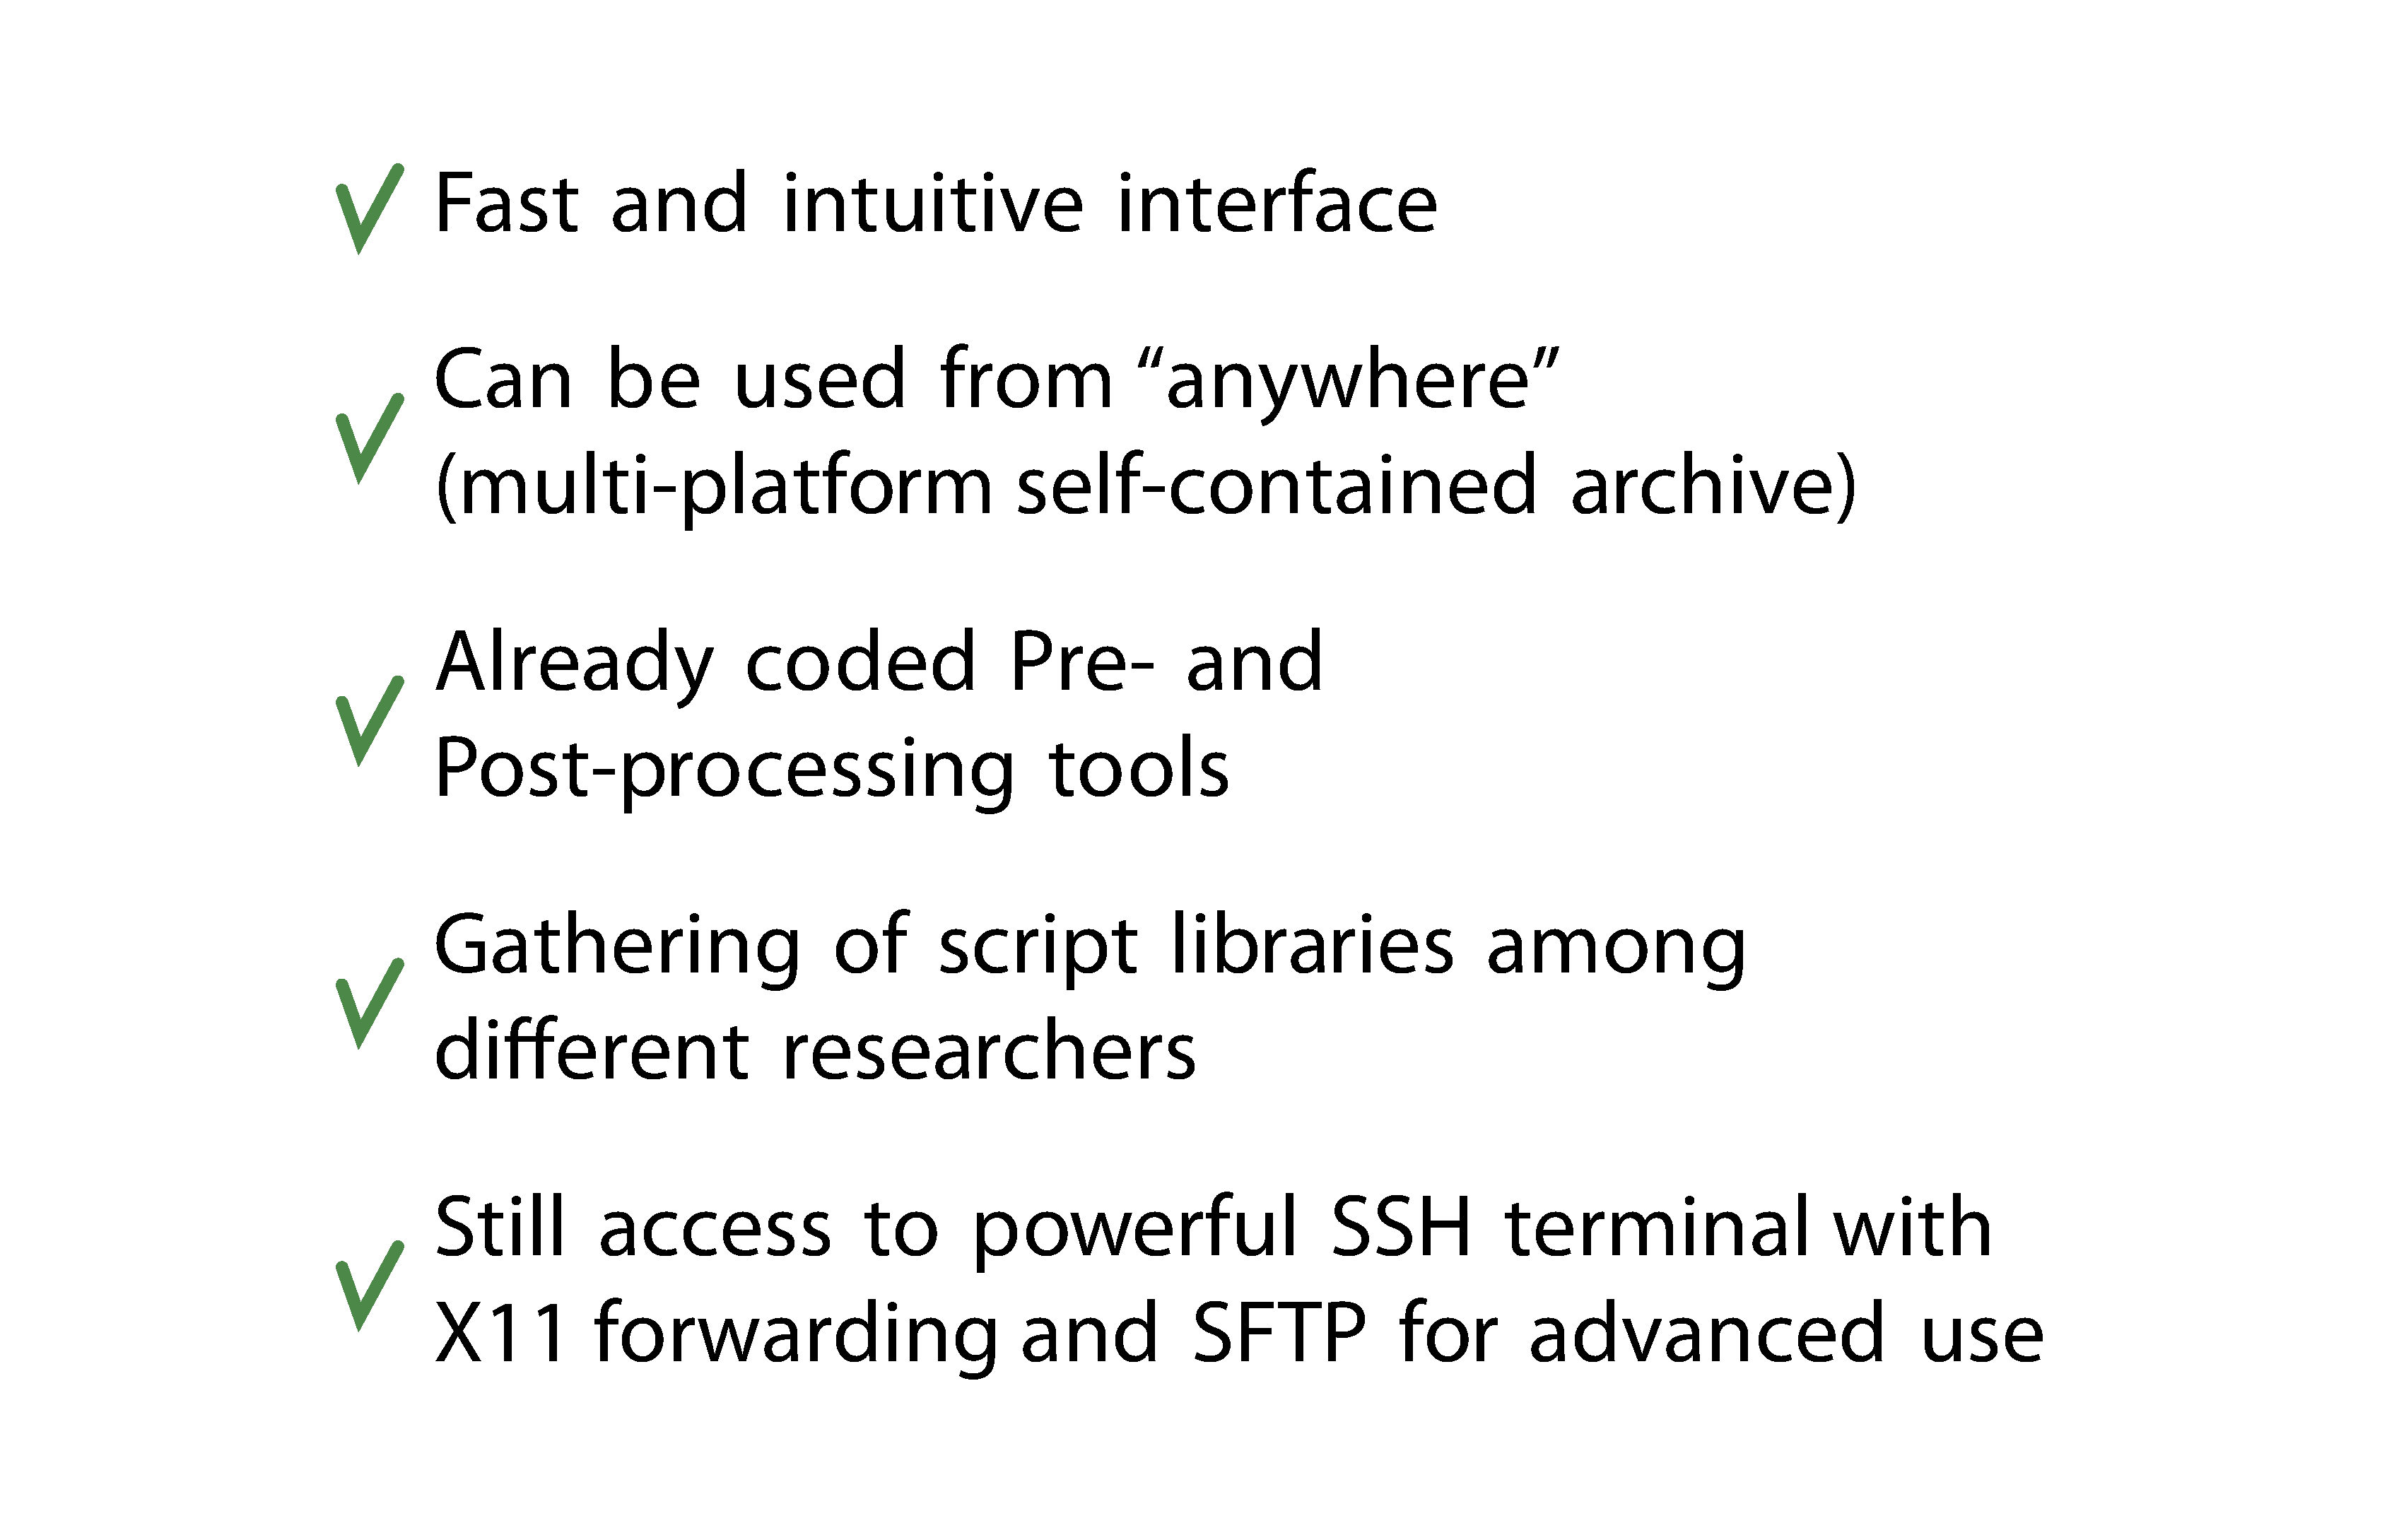
\includegraphics[height=8.25cm]{f0other}\\}
\end{frame}

%%% ----------- I2
%\begin{frame}
% \frametitle{3 examples to use the GUI}
% \centering
%\only<1>{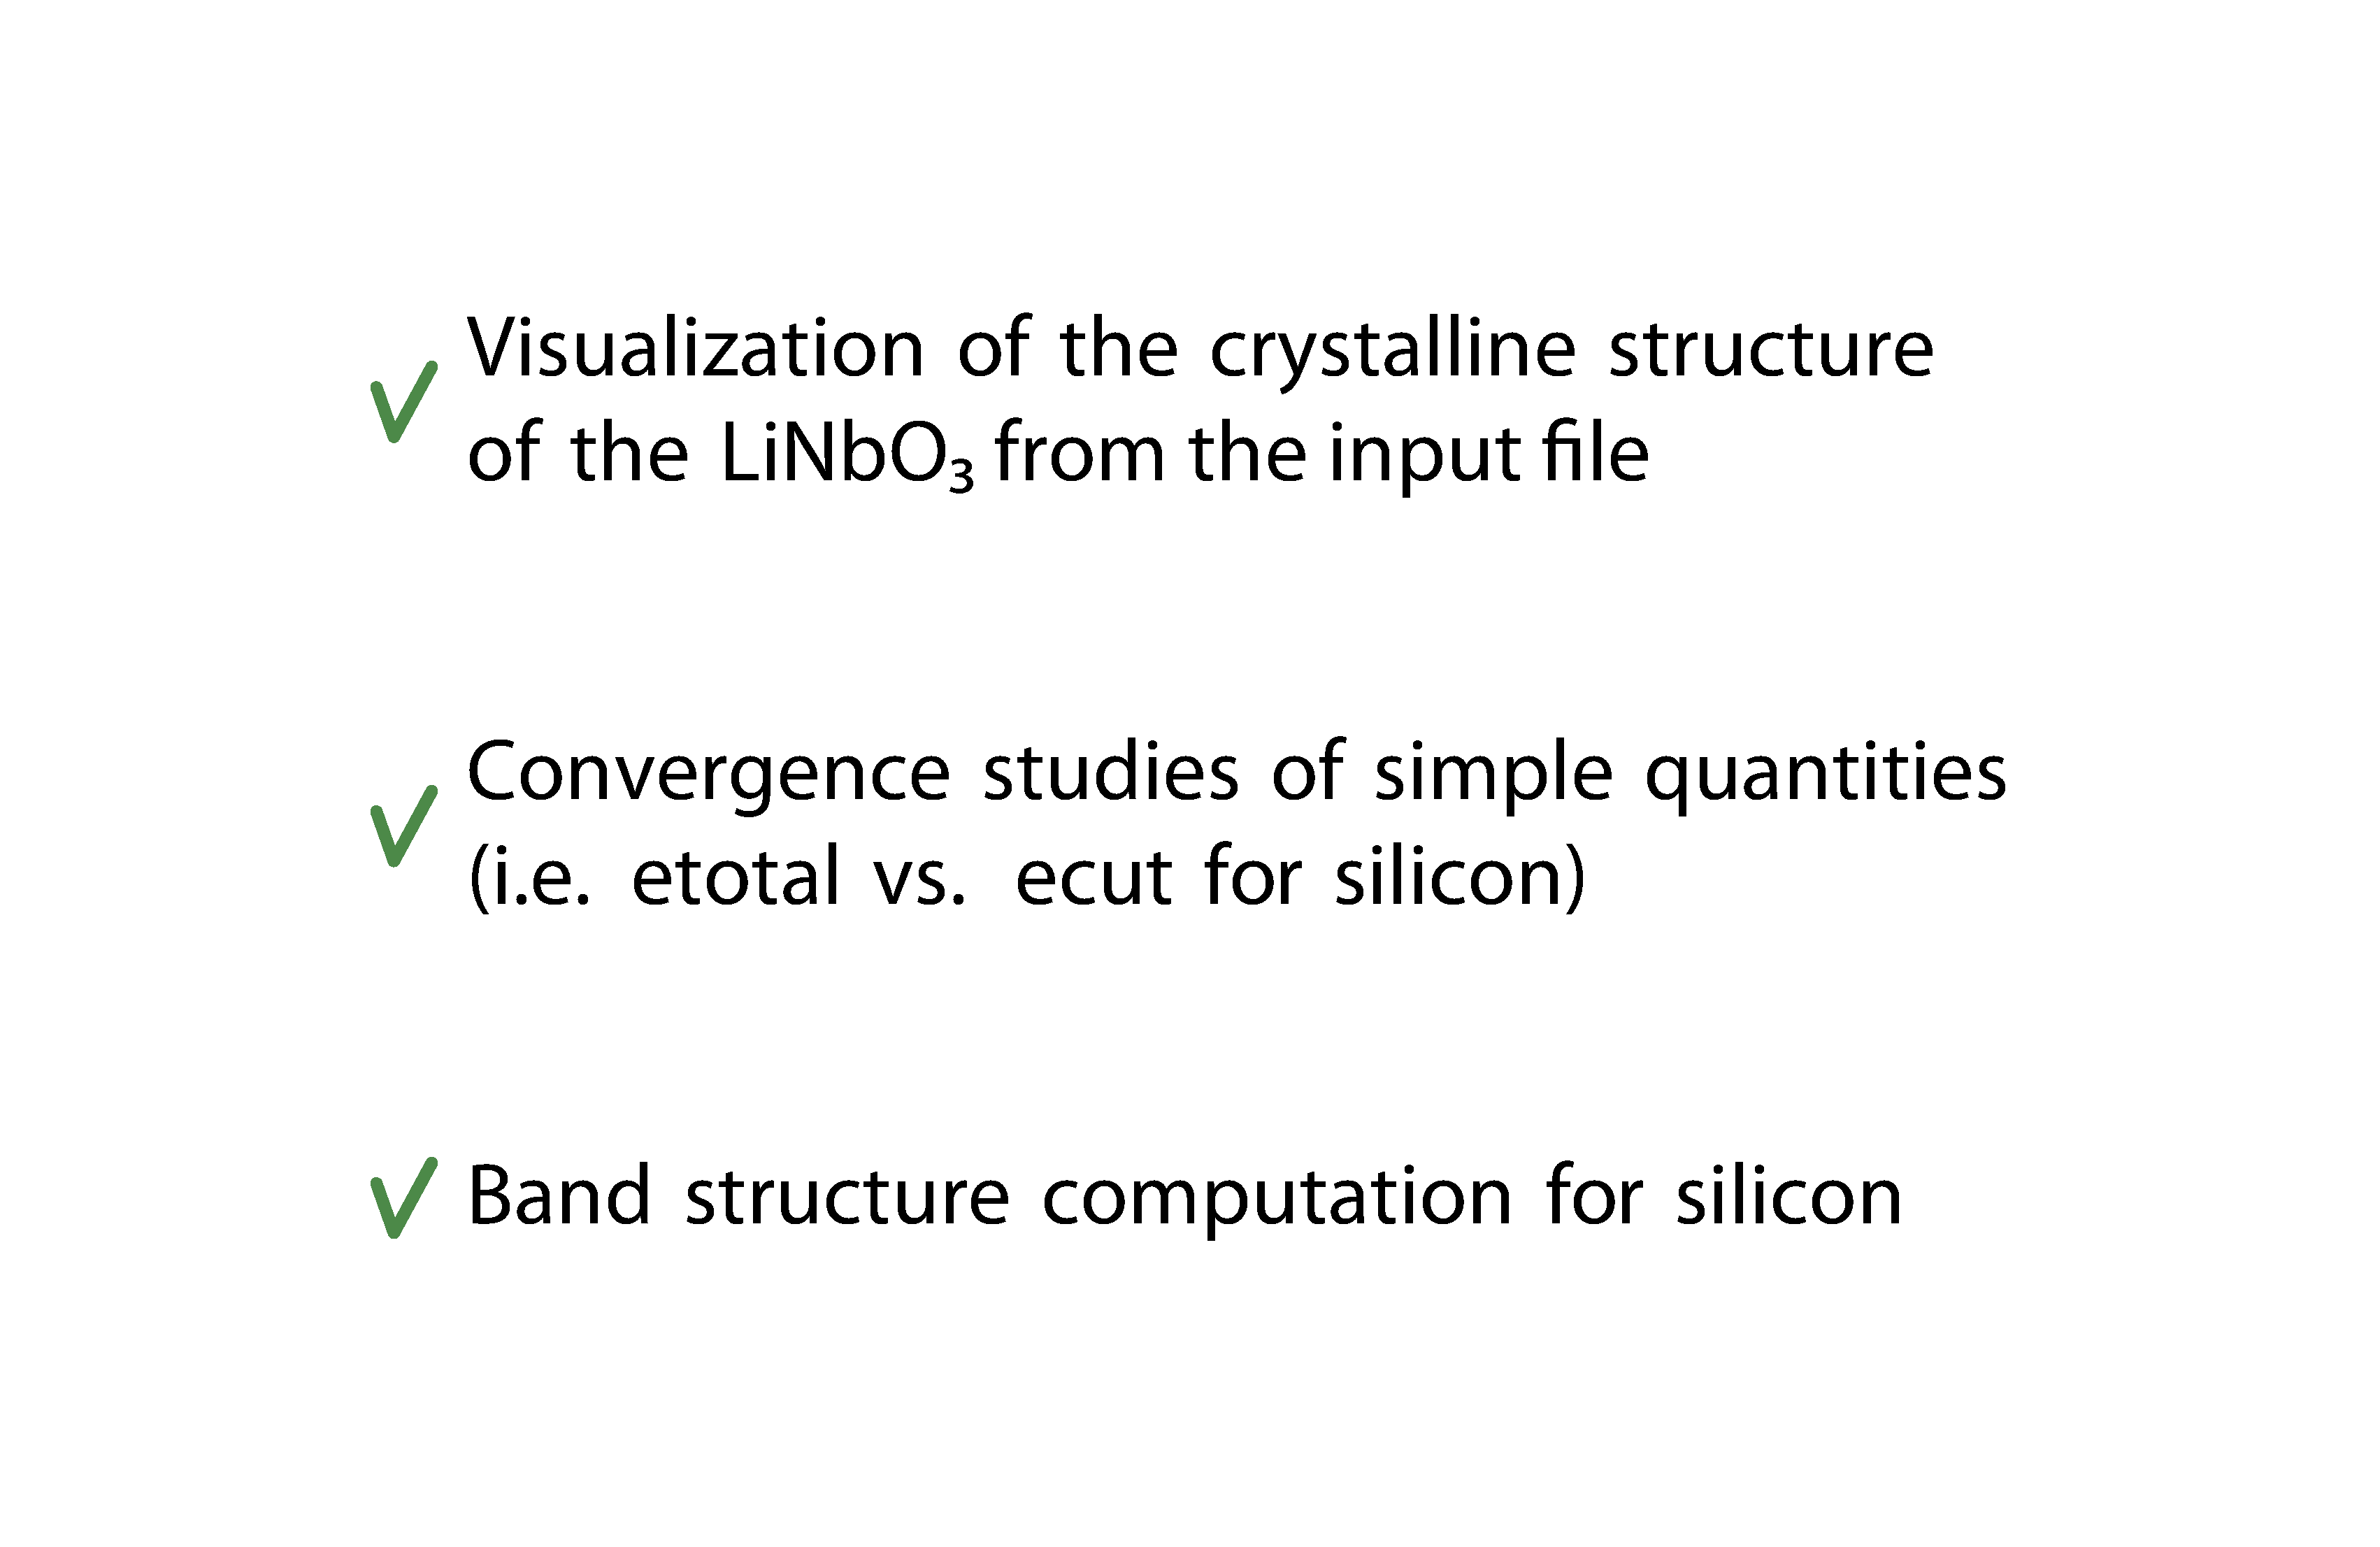
\includegraphics[height=8.25cm]{f0other2}\\}
%\end{frame}

%% ----------- F1
\begin{frame}
 \frametitle{Configurations...}
 \centering
\only<1>{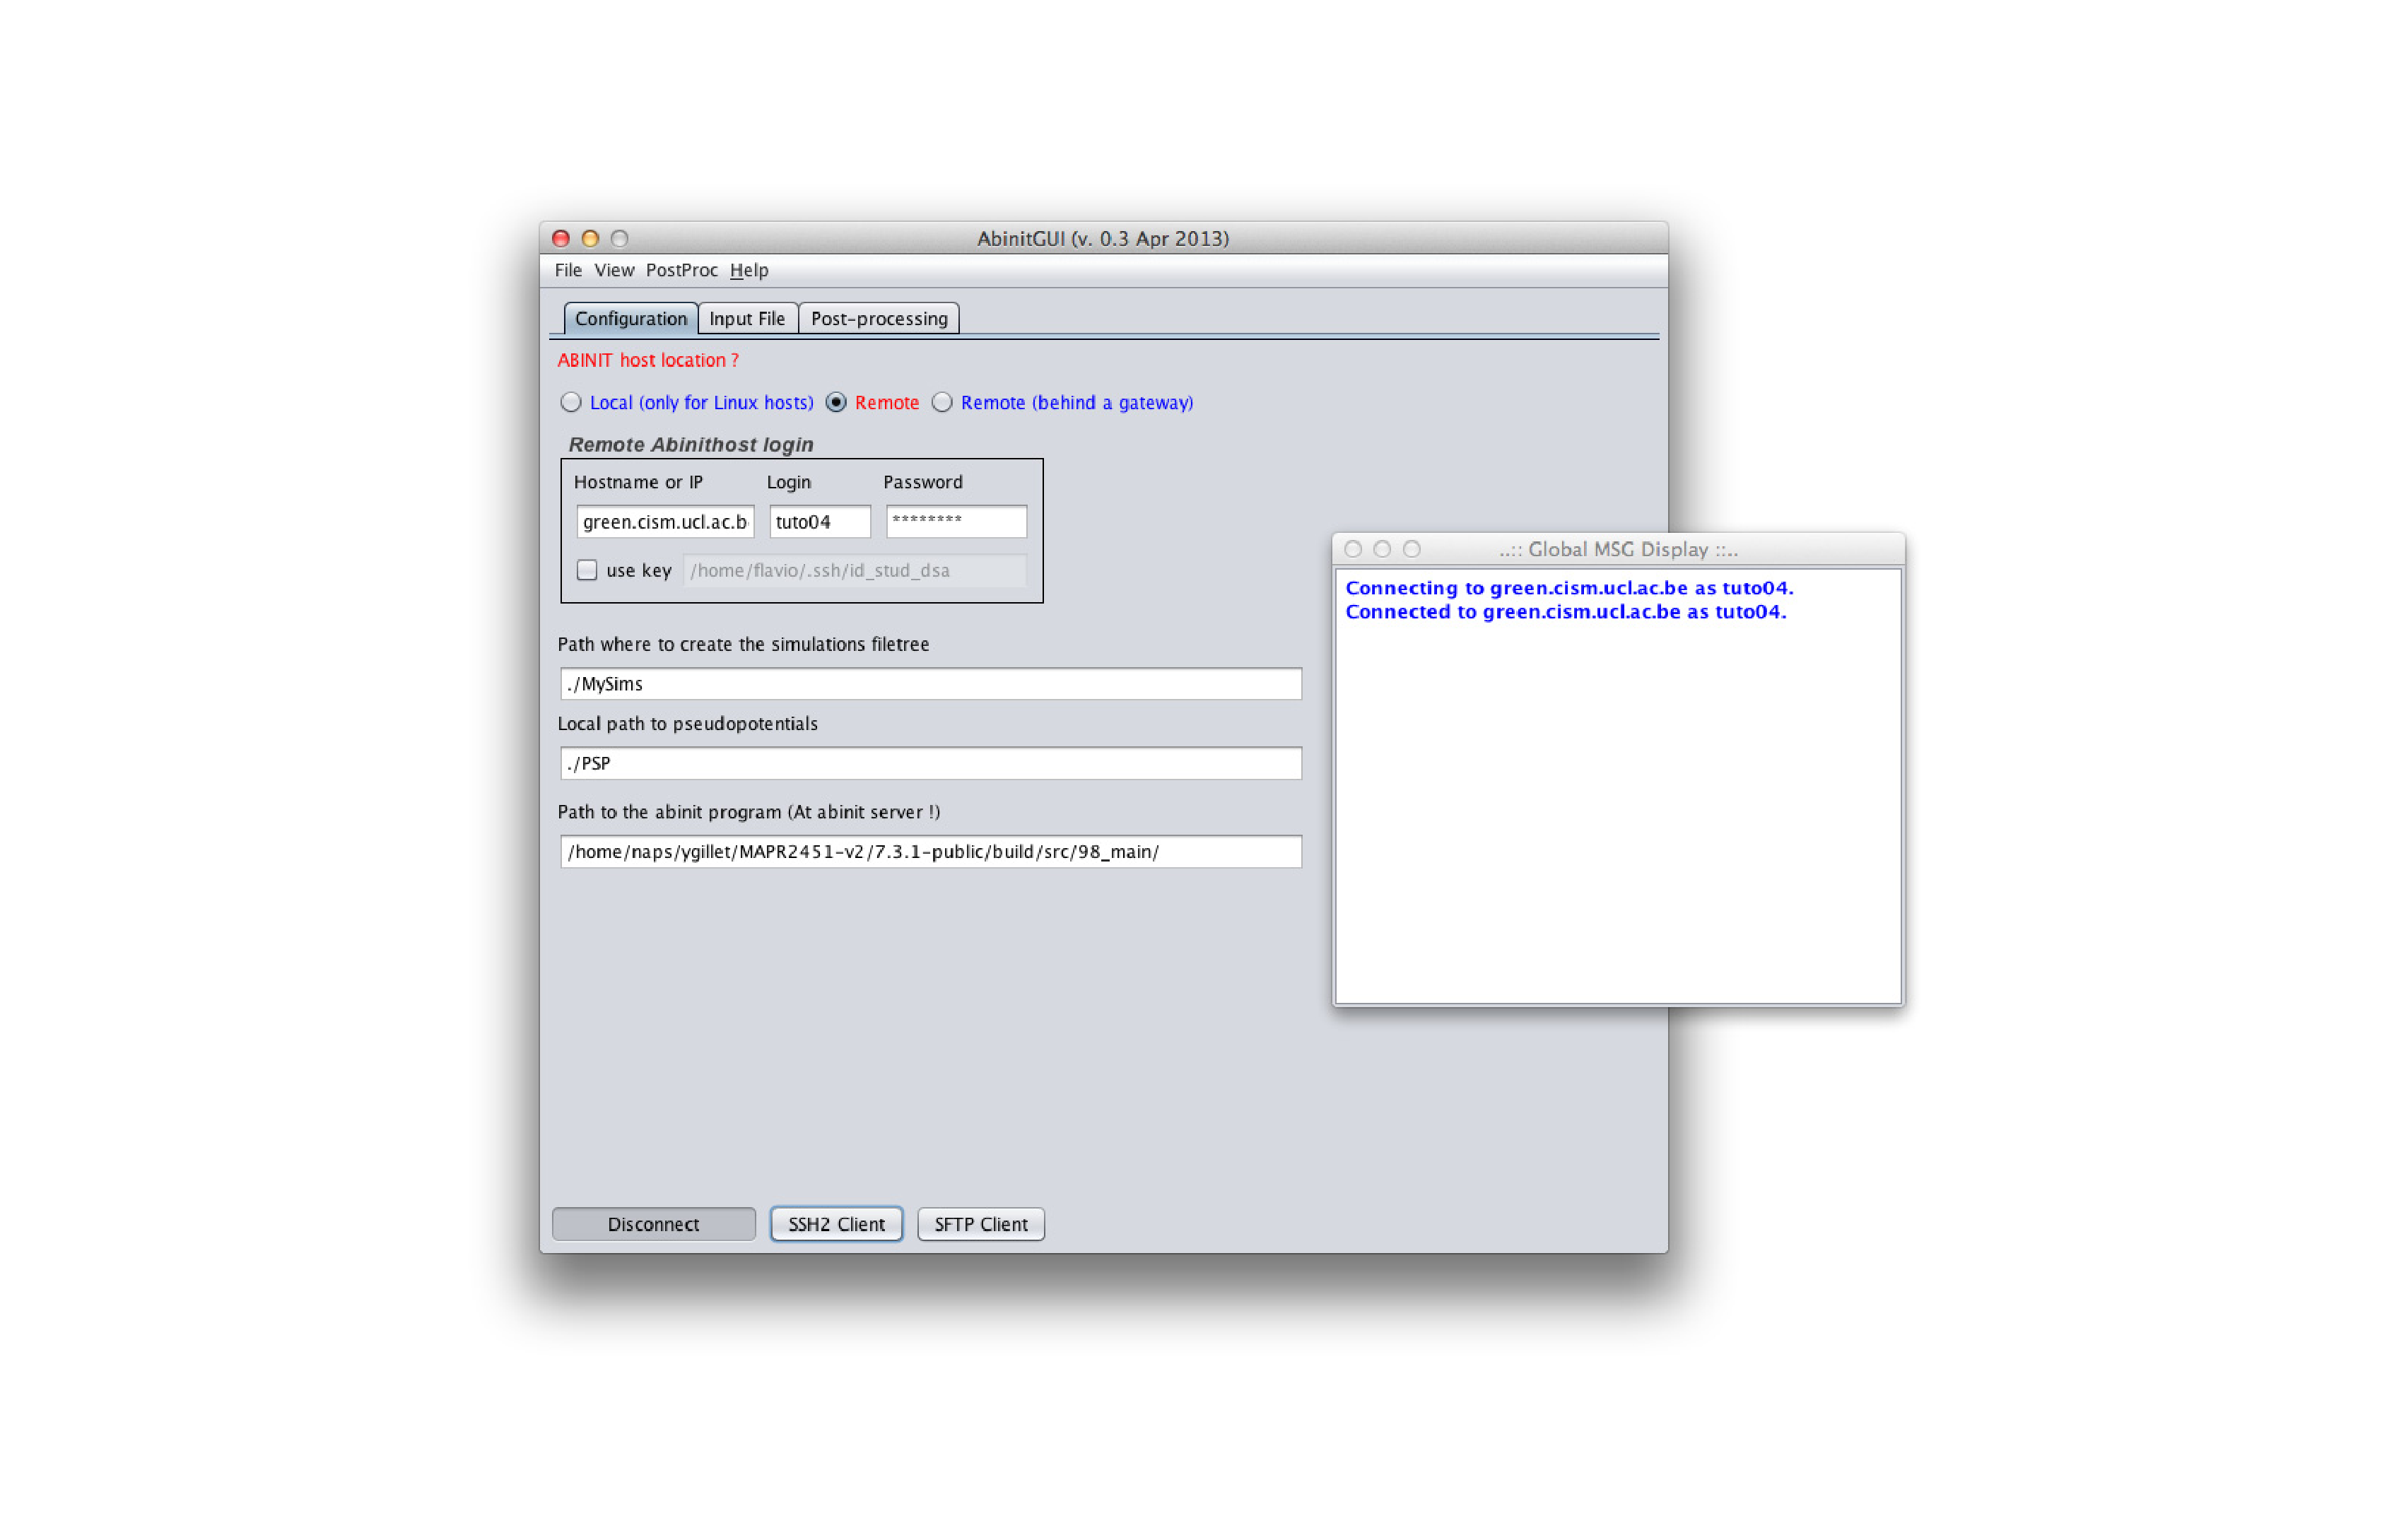
\includegraphics[height=8.25cm]{f1a}\\}
\only<2>{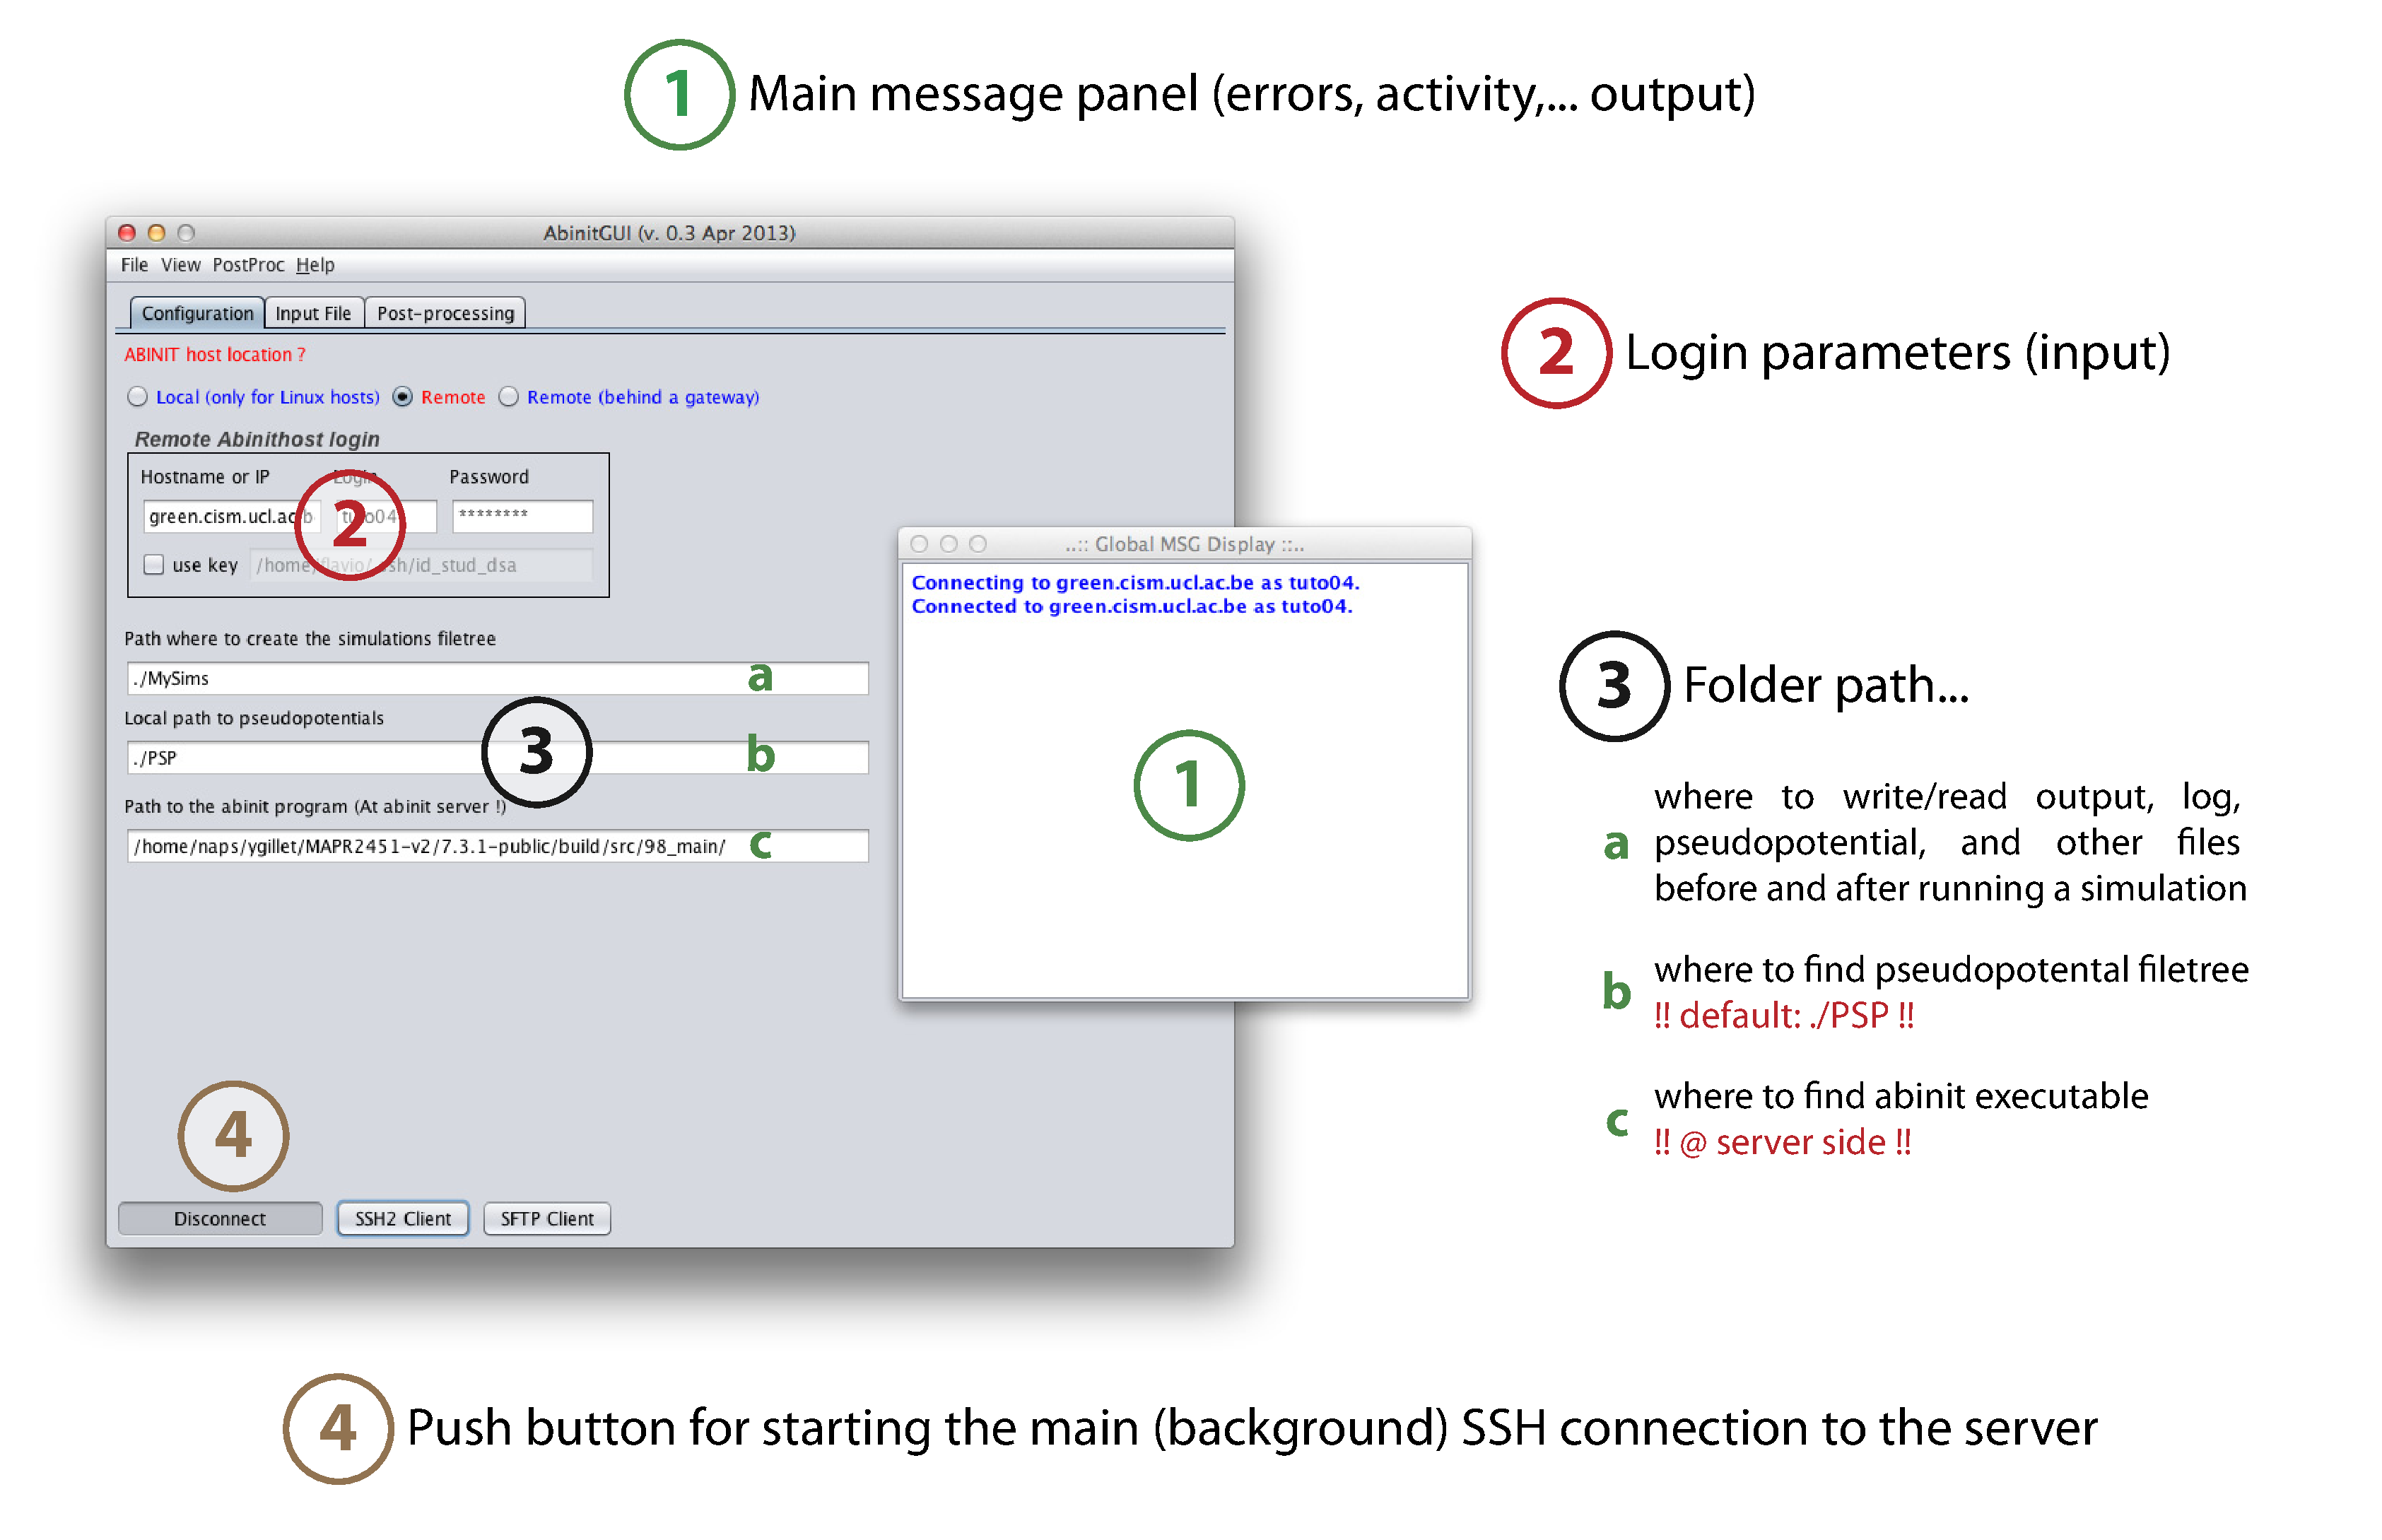
\includegraphics[height=8.25cm]{f1b}\\}
\end{frame}

%% ----------- menu1
\begin{frame}
 \frametitle{Configuration file management}
 \centering
 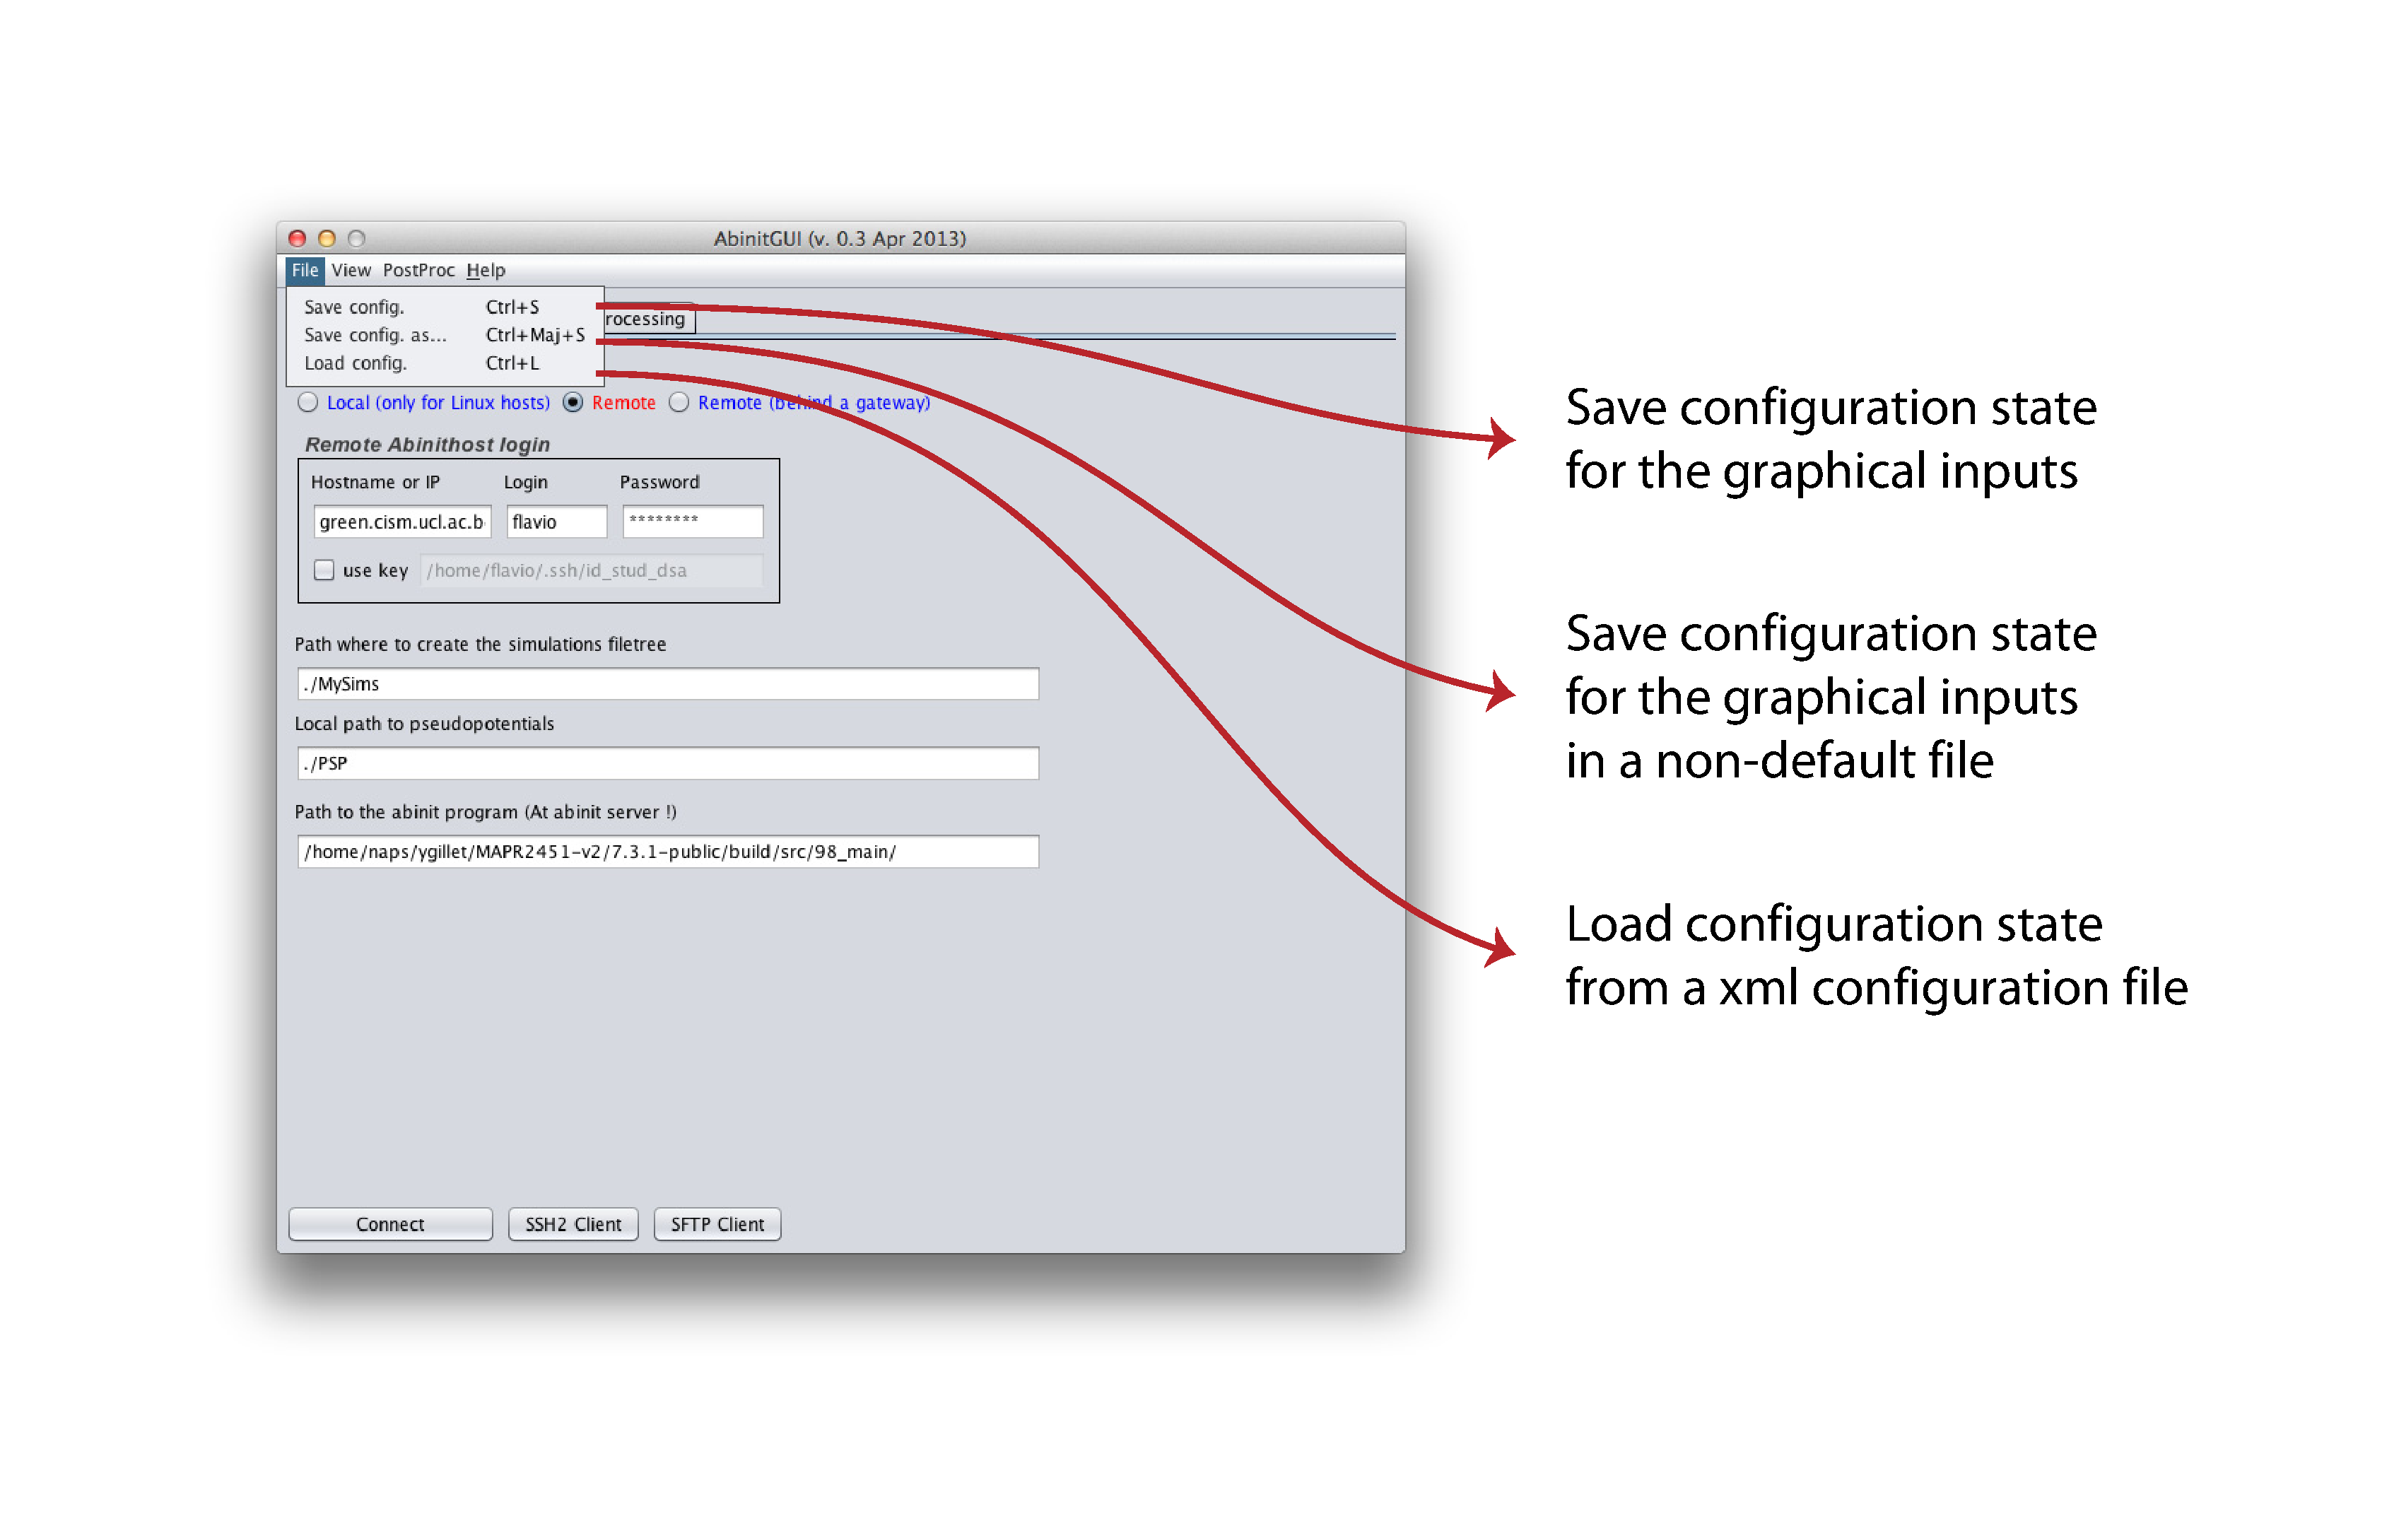
\includegraphics[height=8.25cm]{menu1}
\end{frame}

%% ----------- F2
\begin{frame}
 \frametitle{SSH}
 \centering
 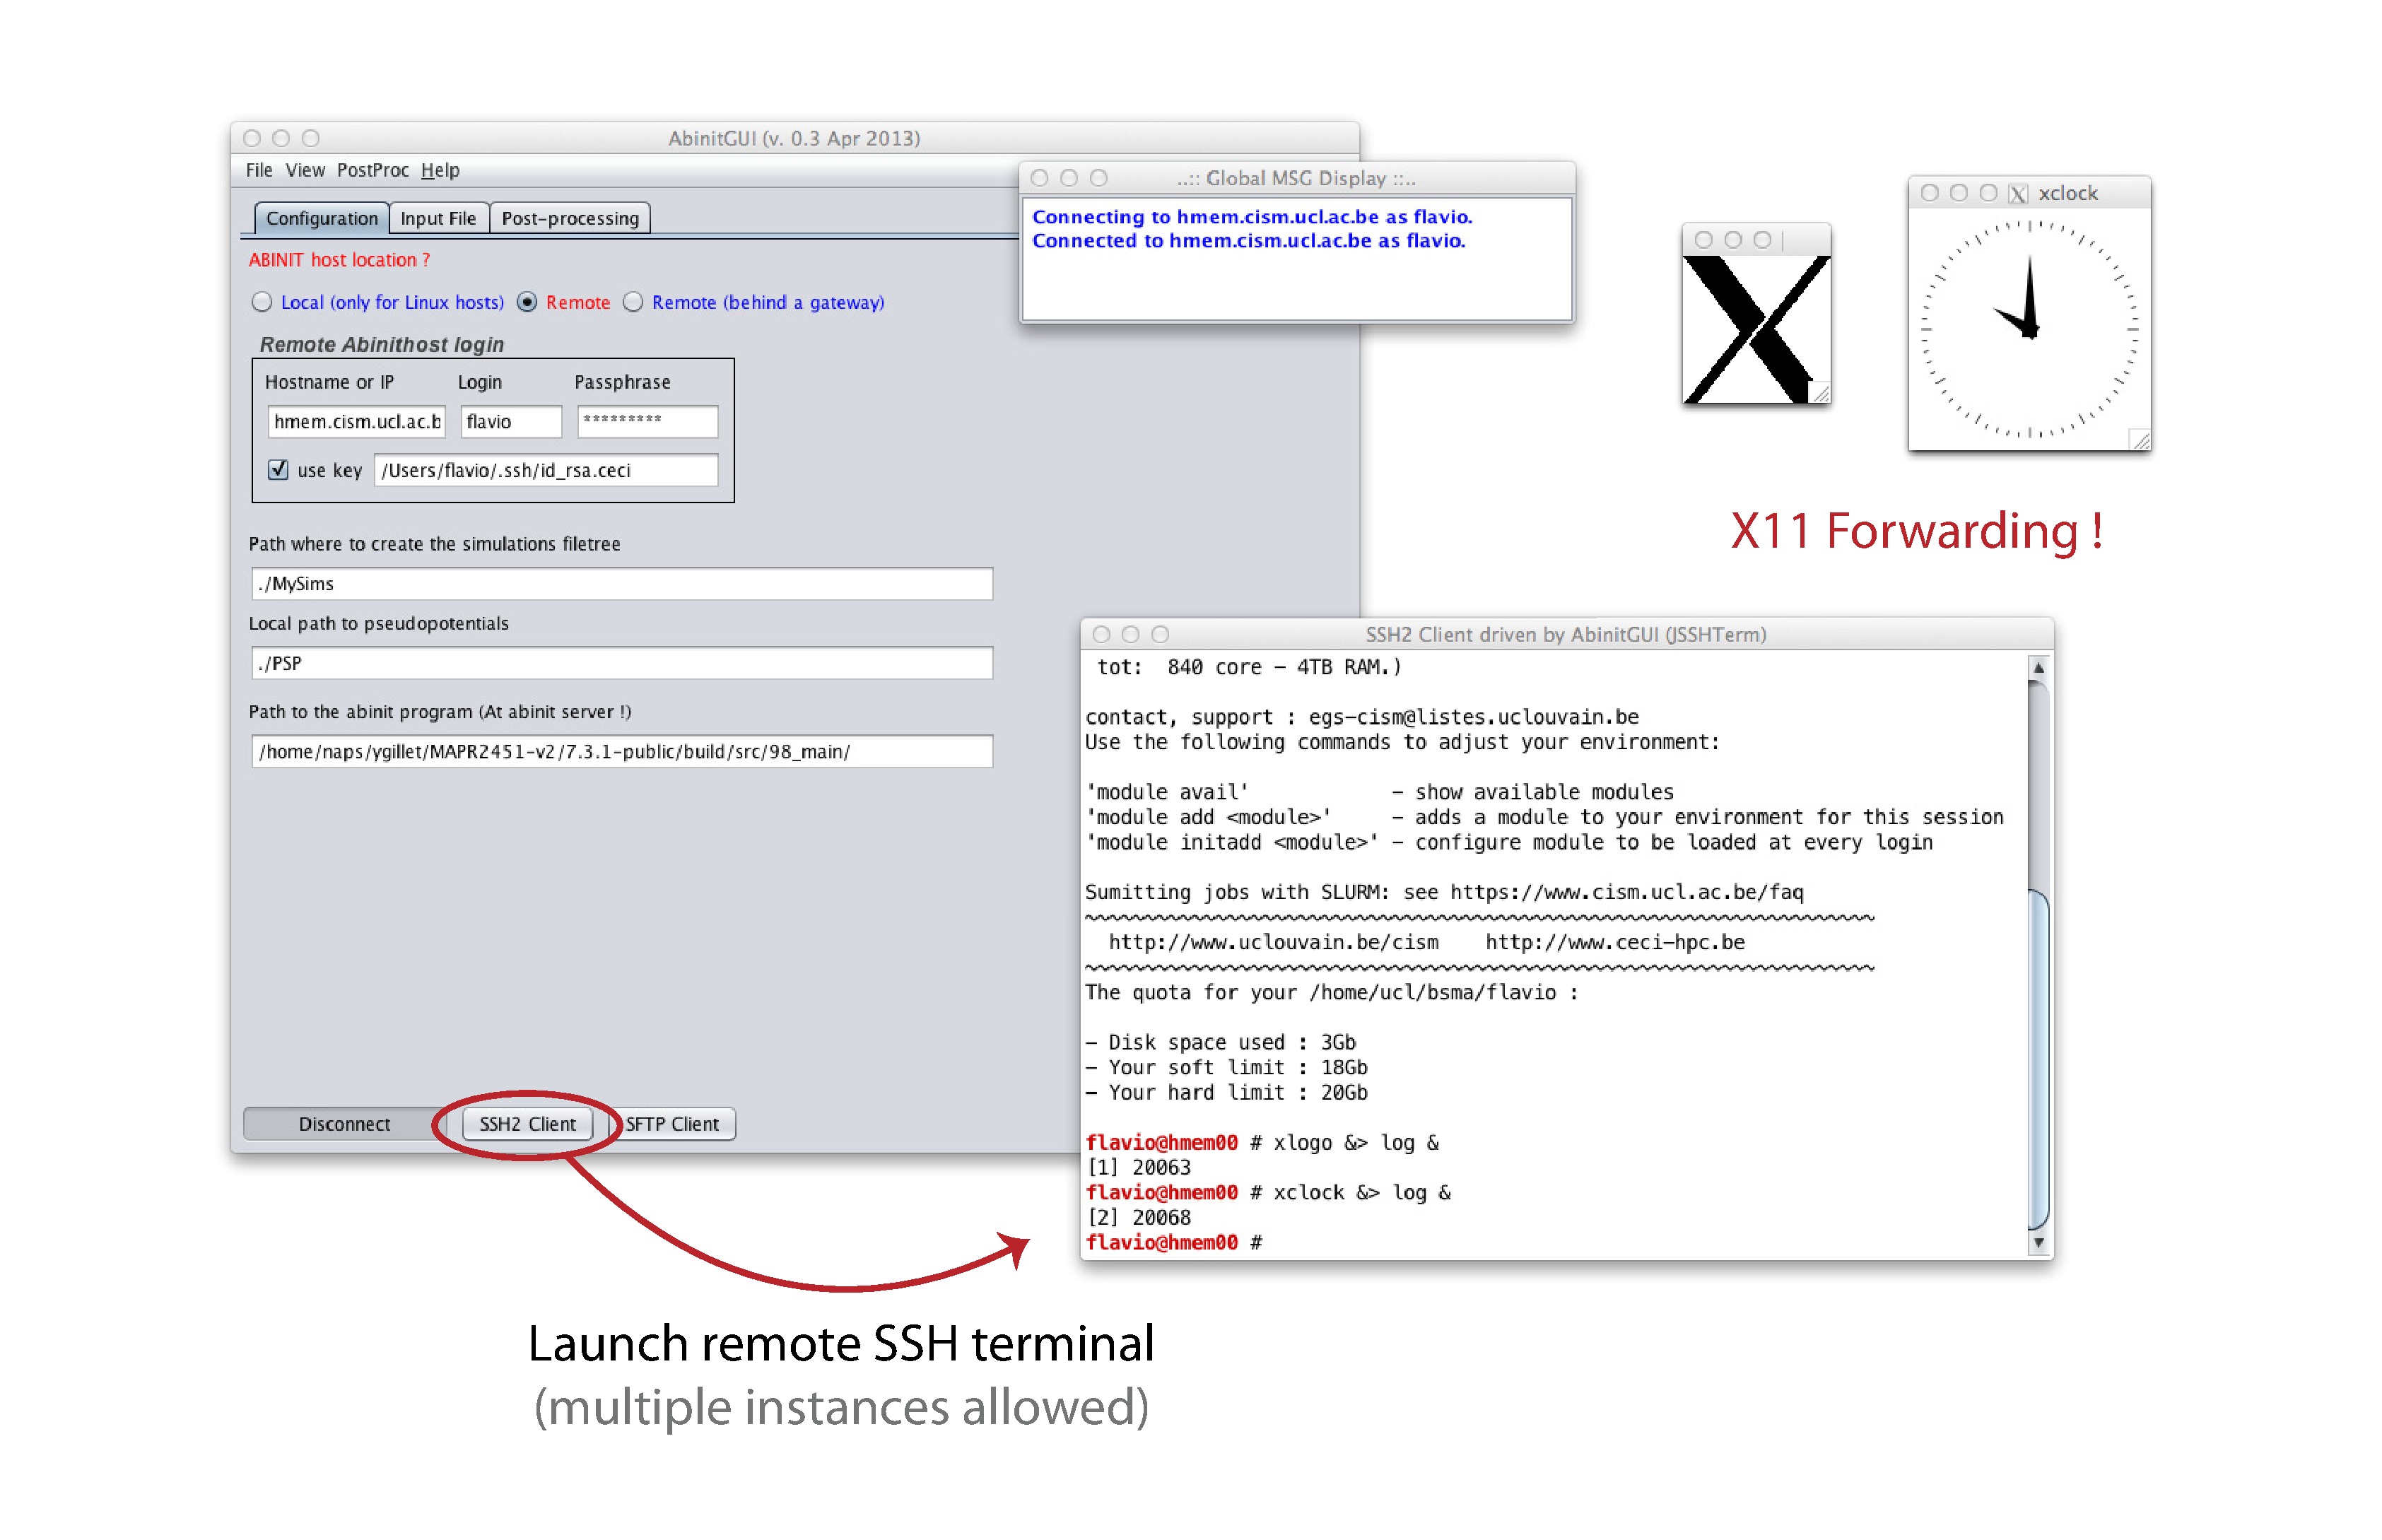
\includegraphics[height=8.25cm]{f4}
\end{frame}

%% ----------- F3
\begin{frame}
 \frametitle{SFTP}
 \centering
 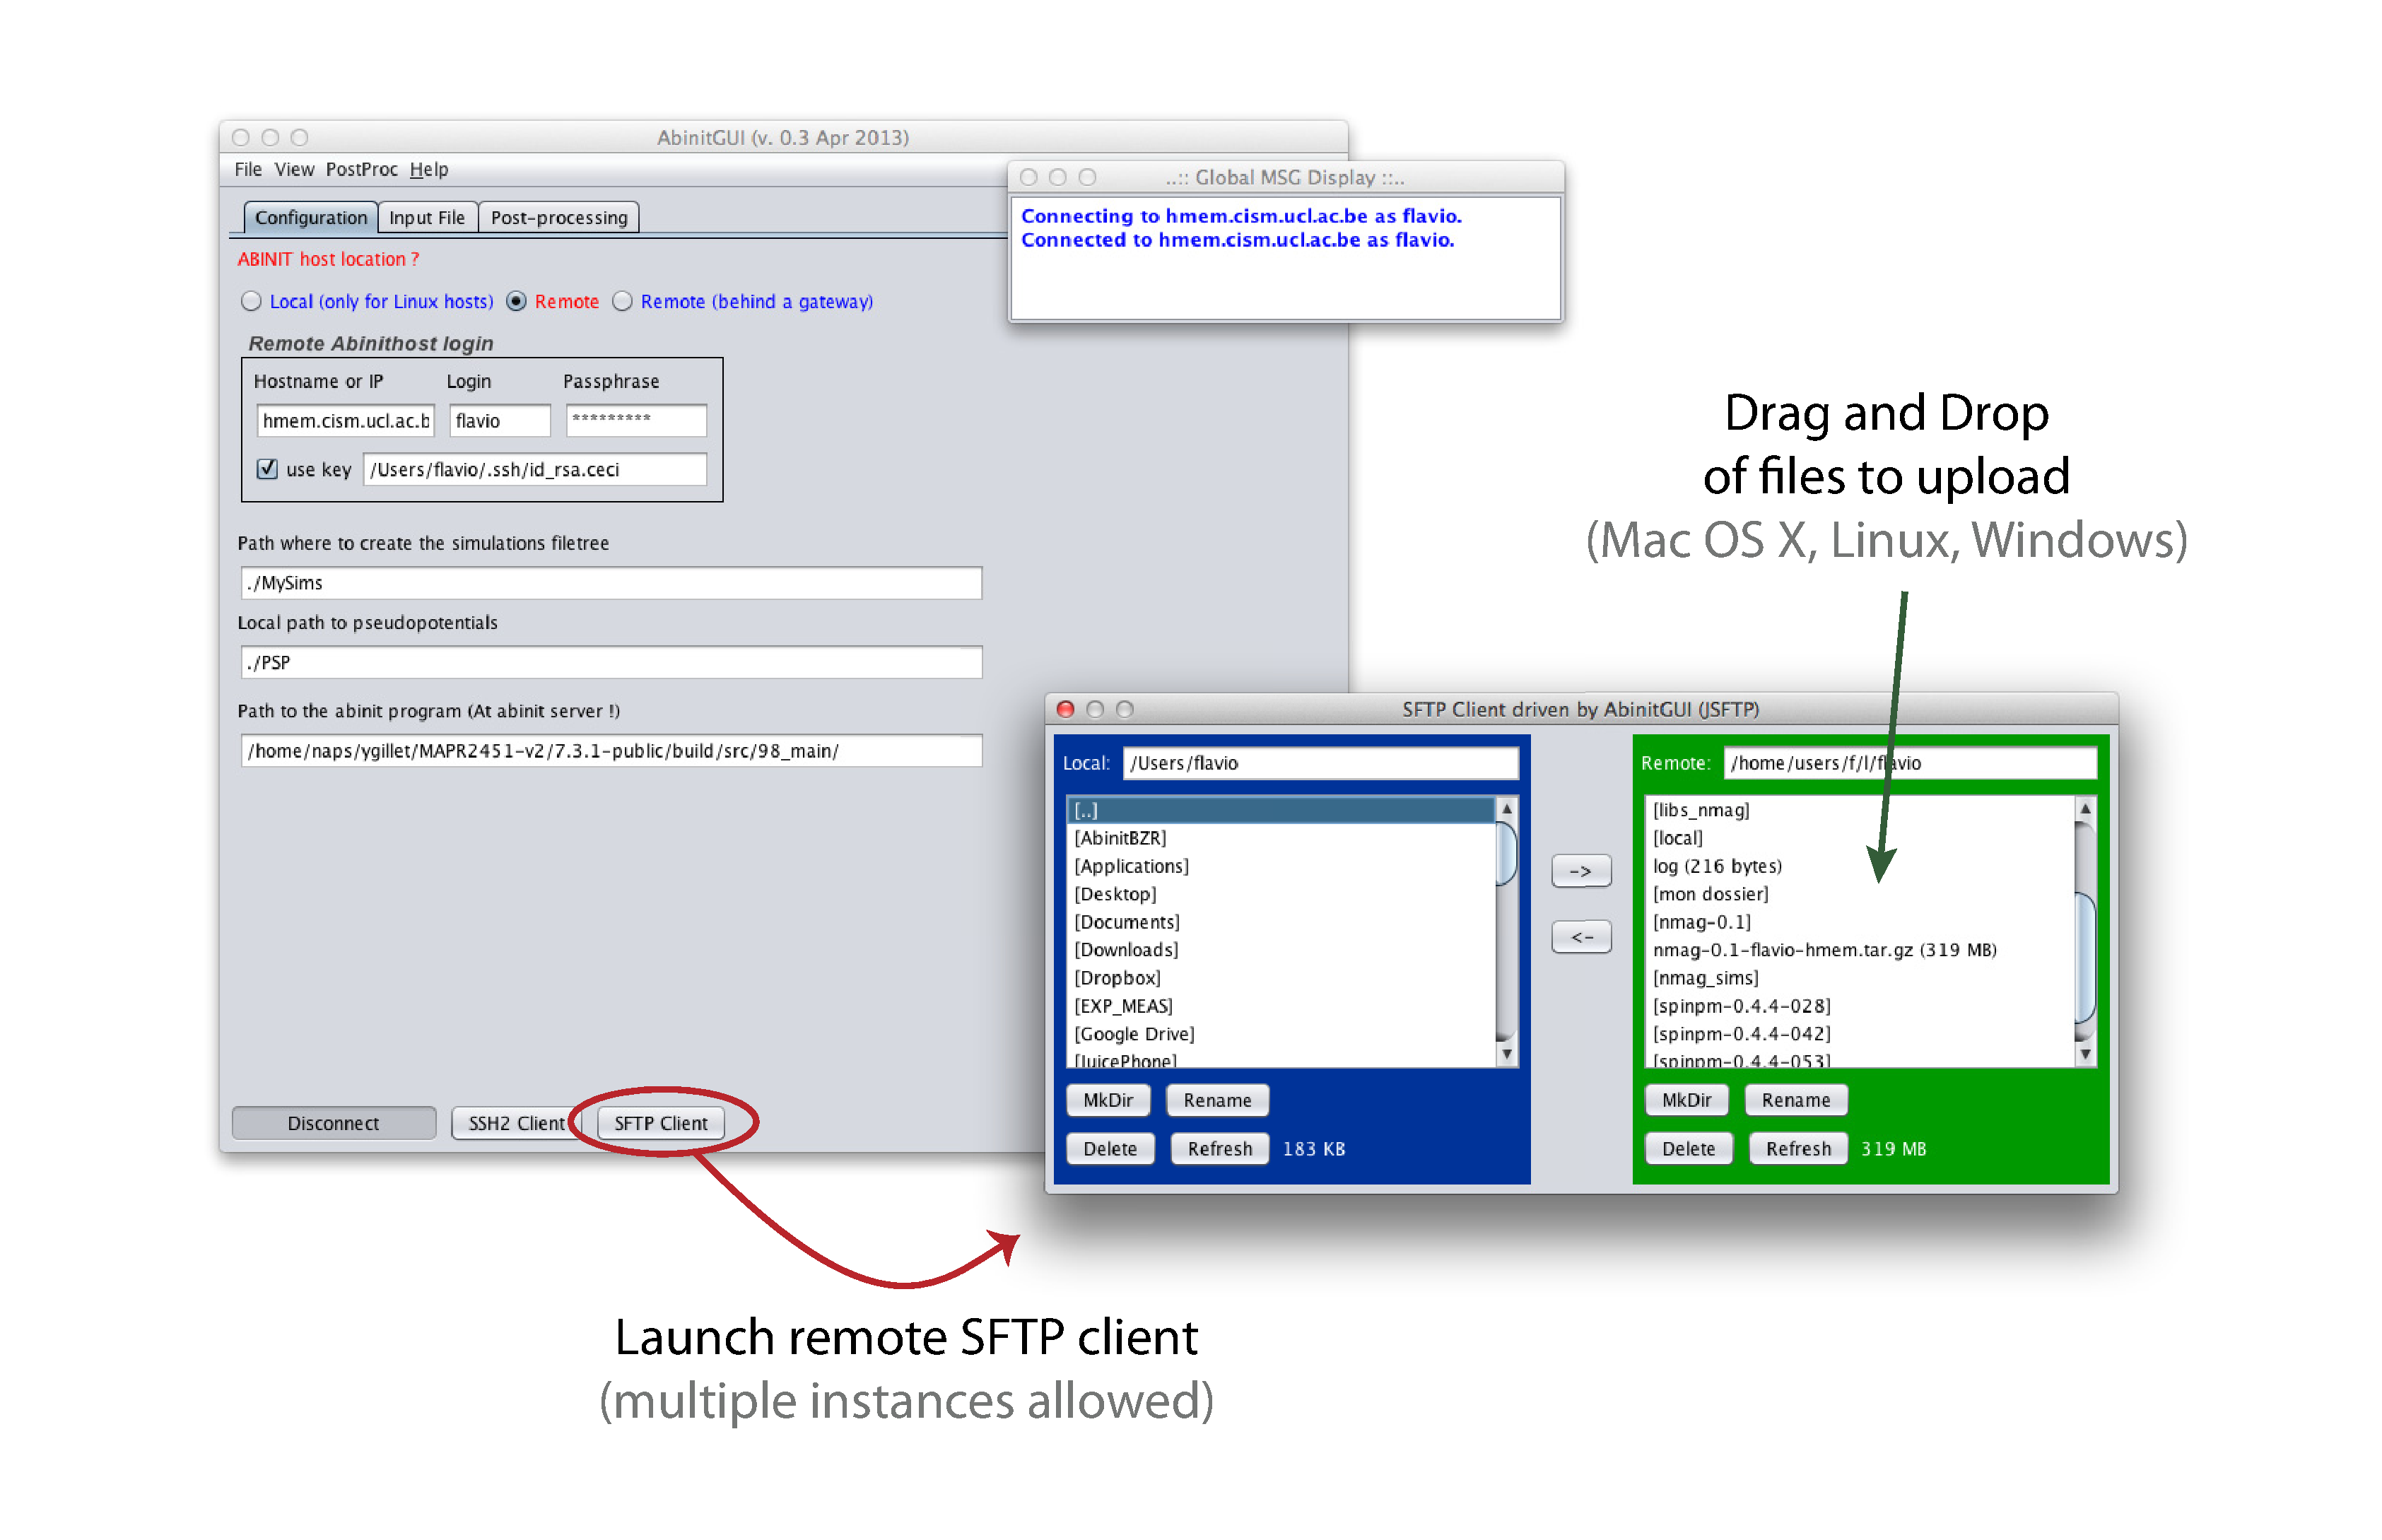
\includegraphics[height=8.25cm]{f5}
\end{frame}

%%% ----------- F6
%\begin{frame}
% \frametitle{Menus...}
%\centering
%\only<1>{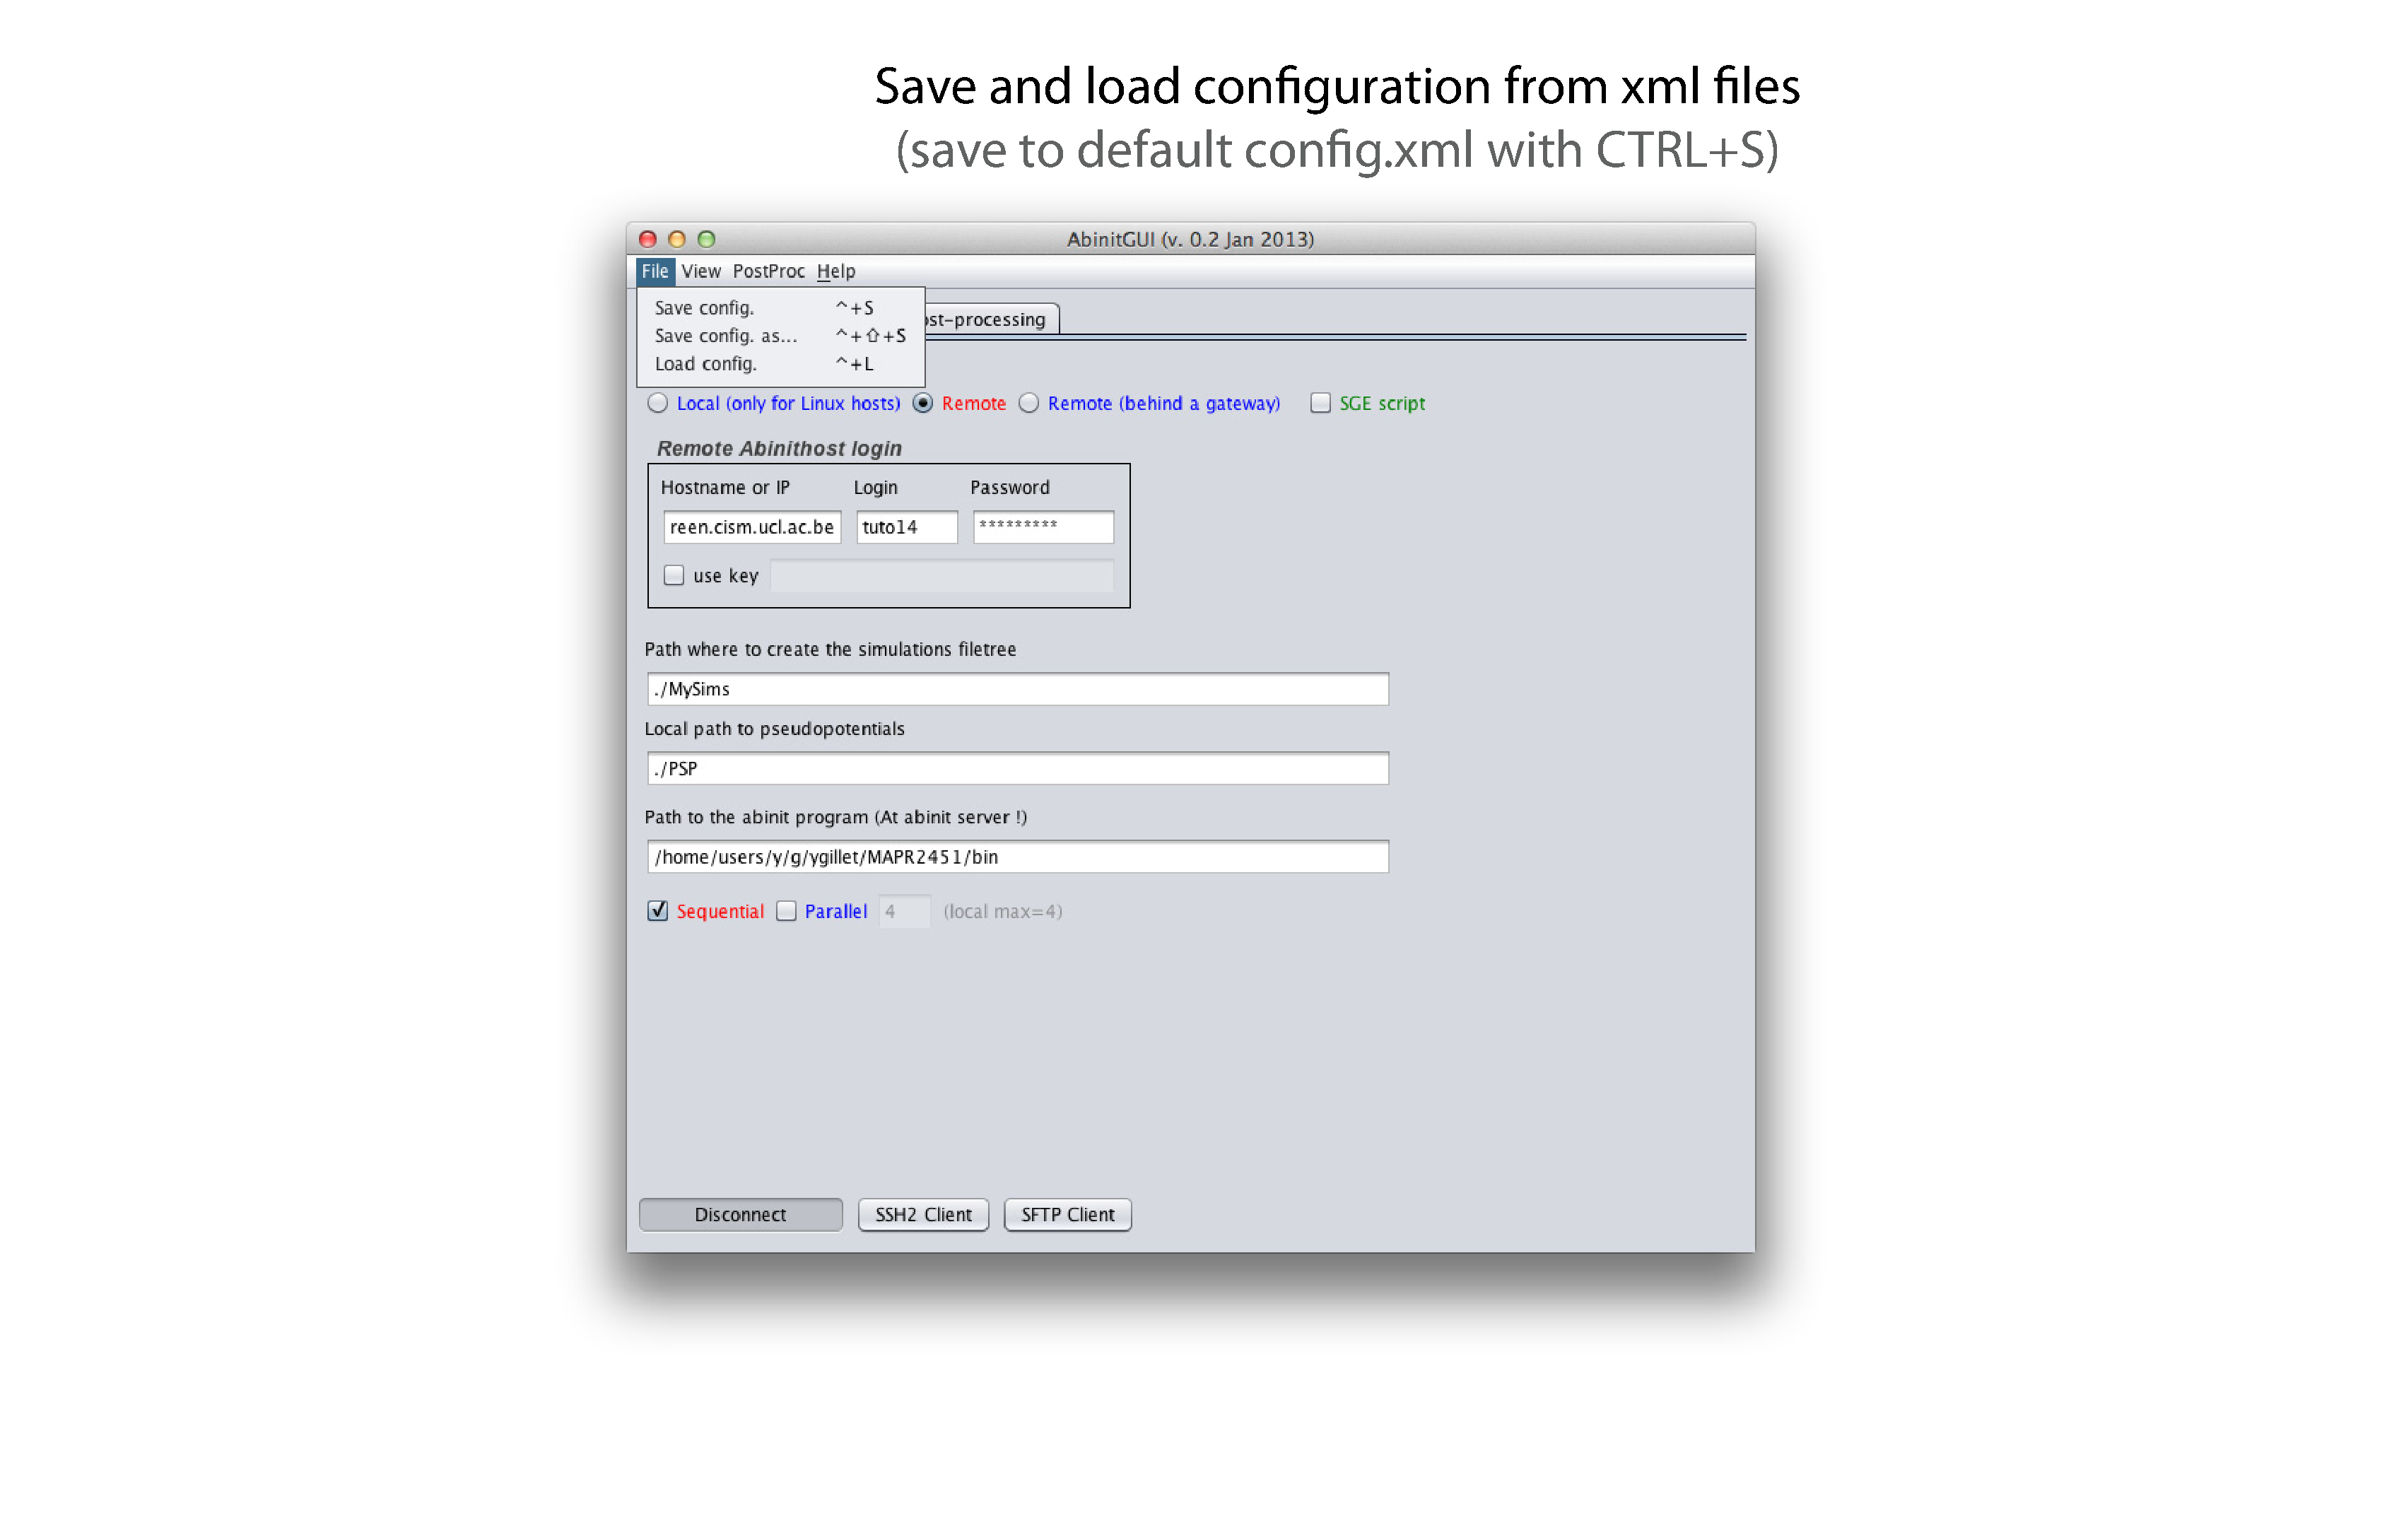
\includegraphics[height=8.25cm]{f6a}\\}
%\only<2>{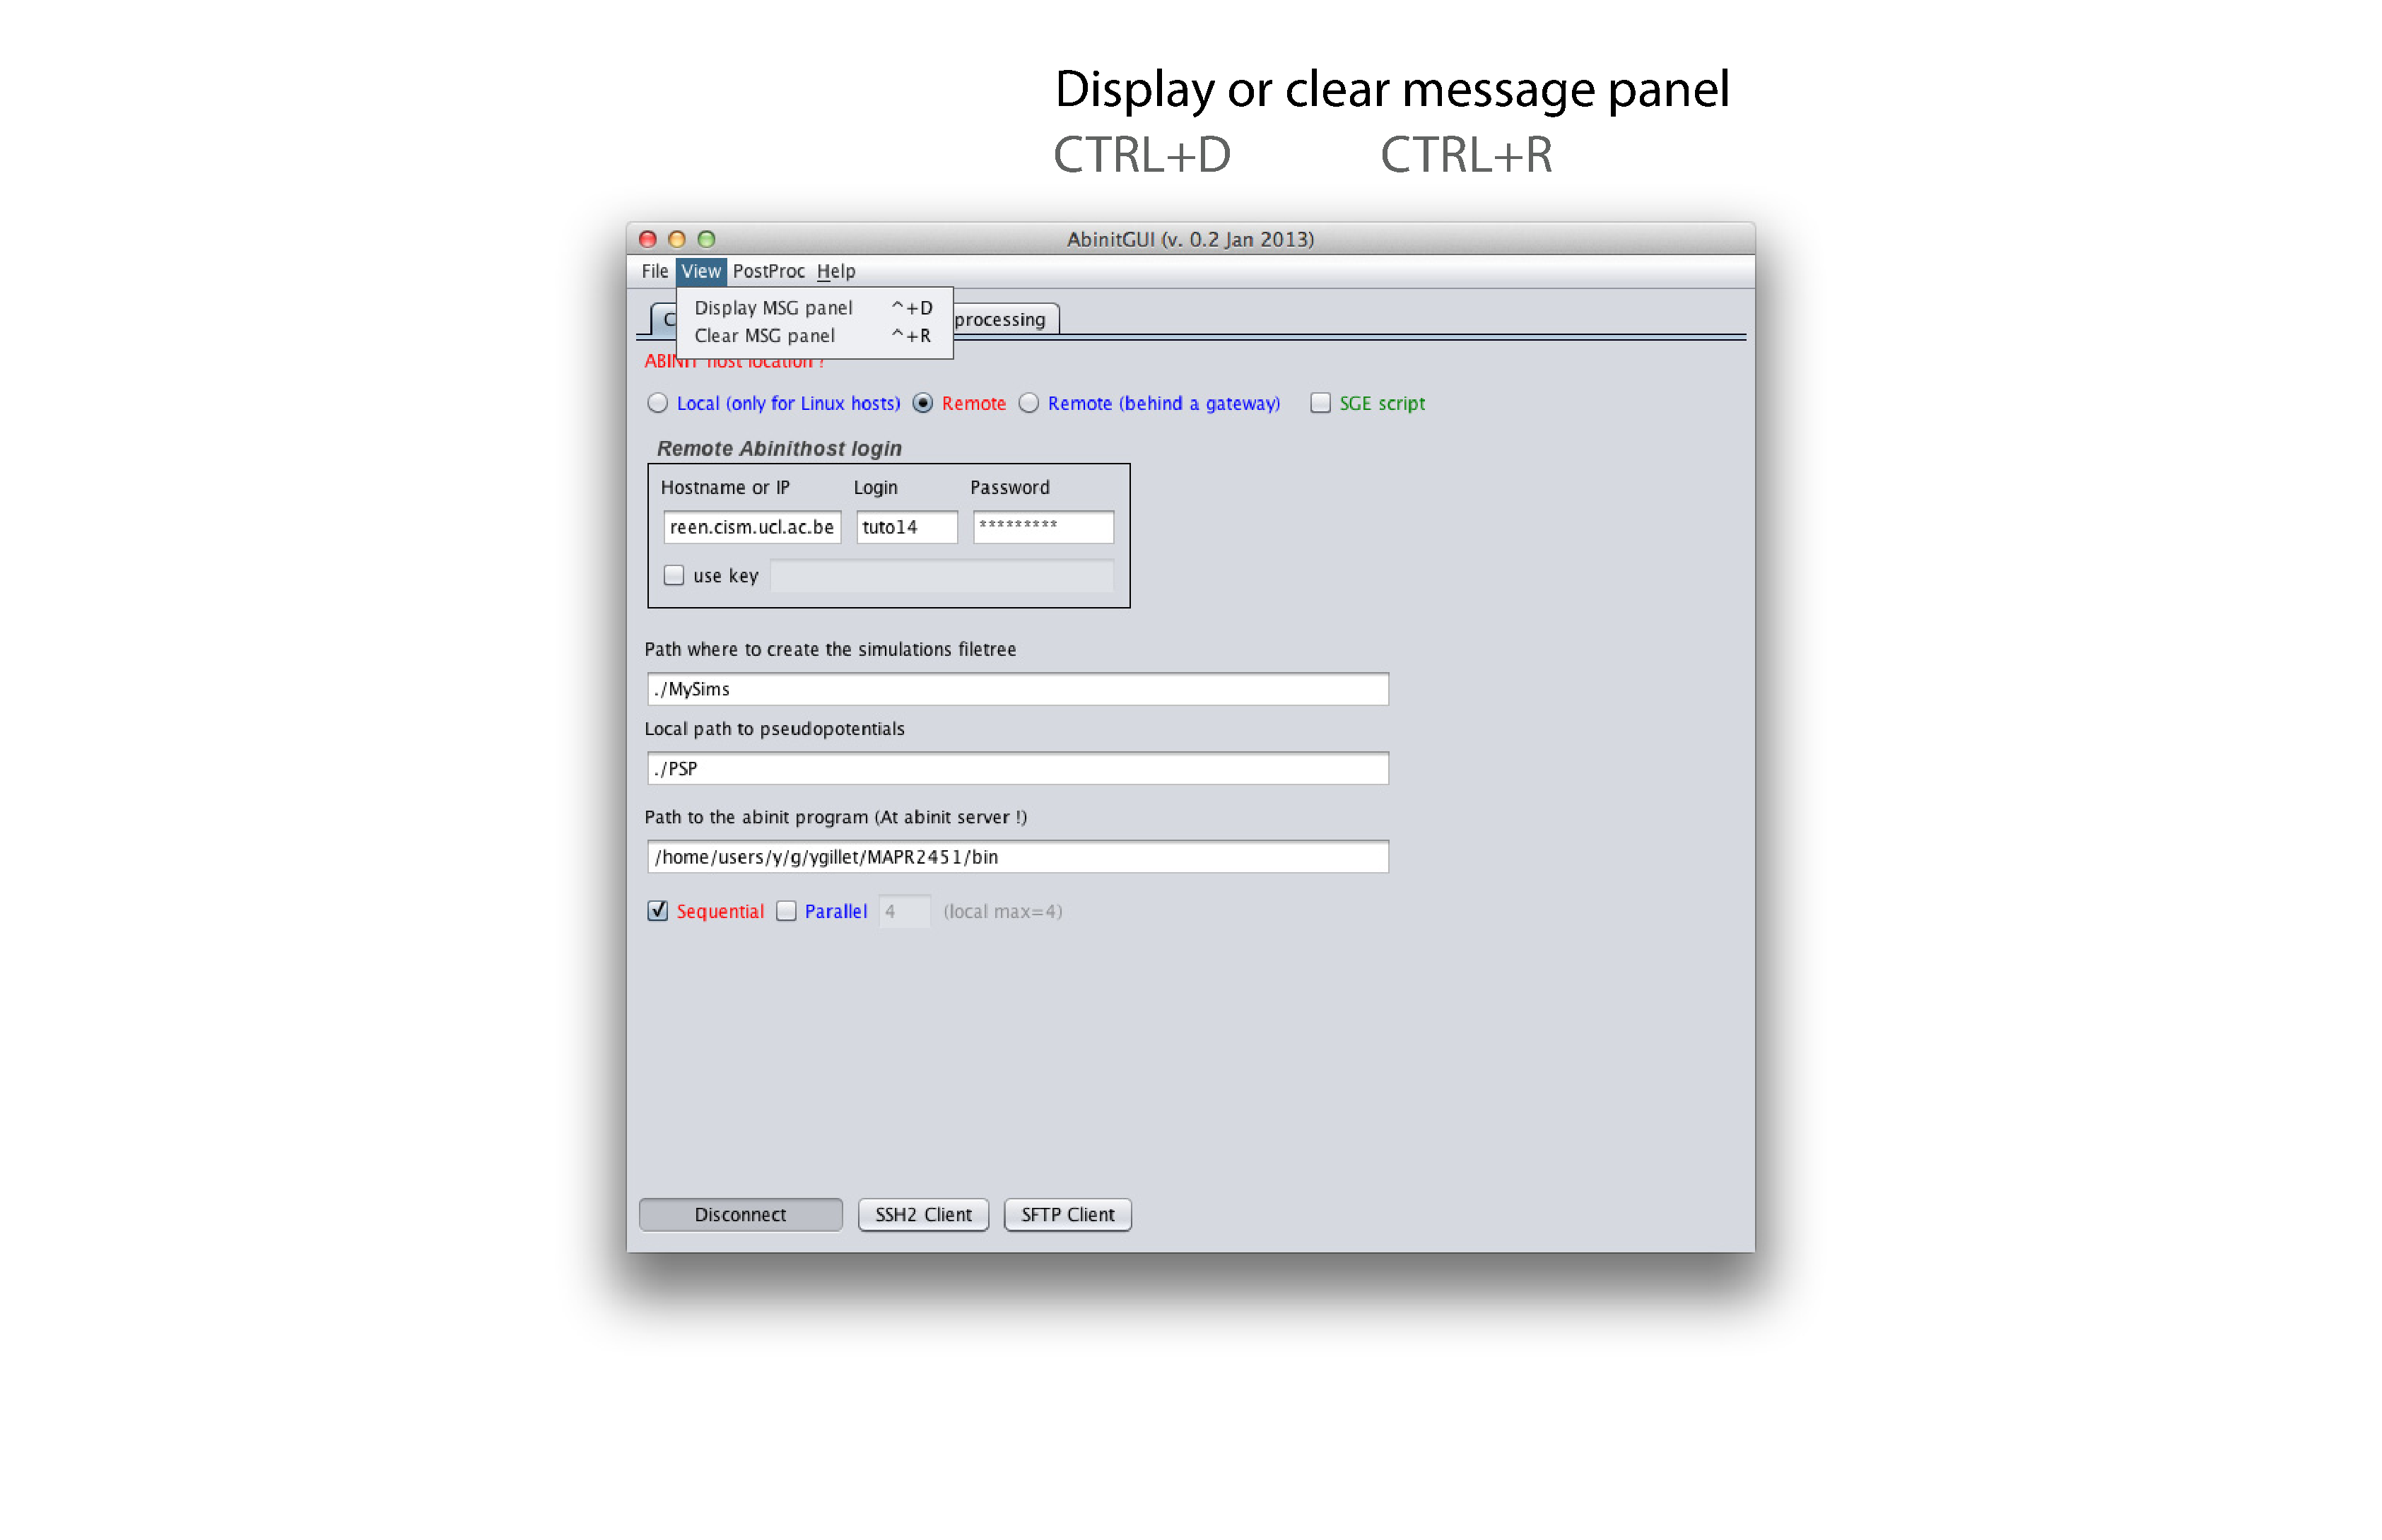
\includegraphics[height=8.25cm]{f6b}\\}
%\only<3>{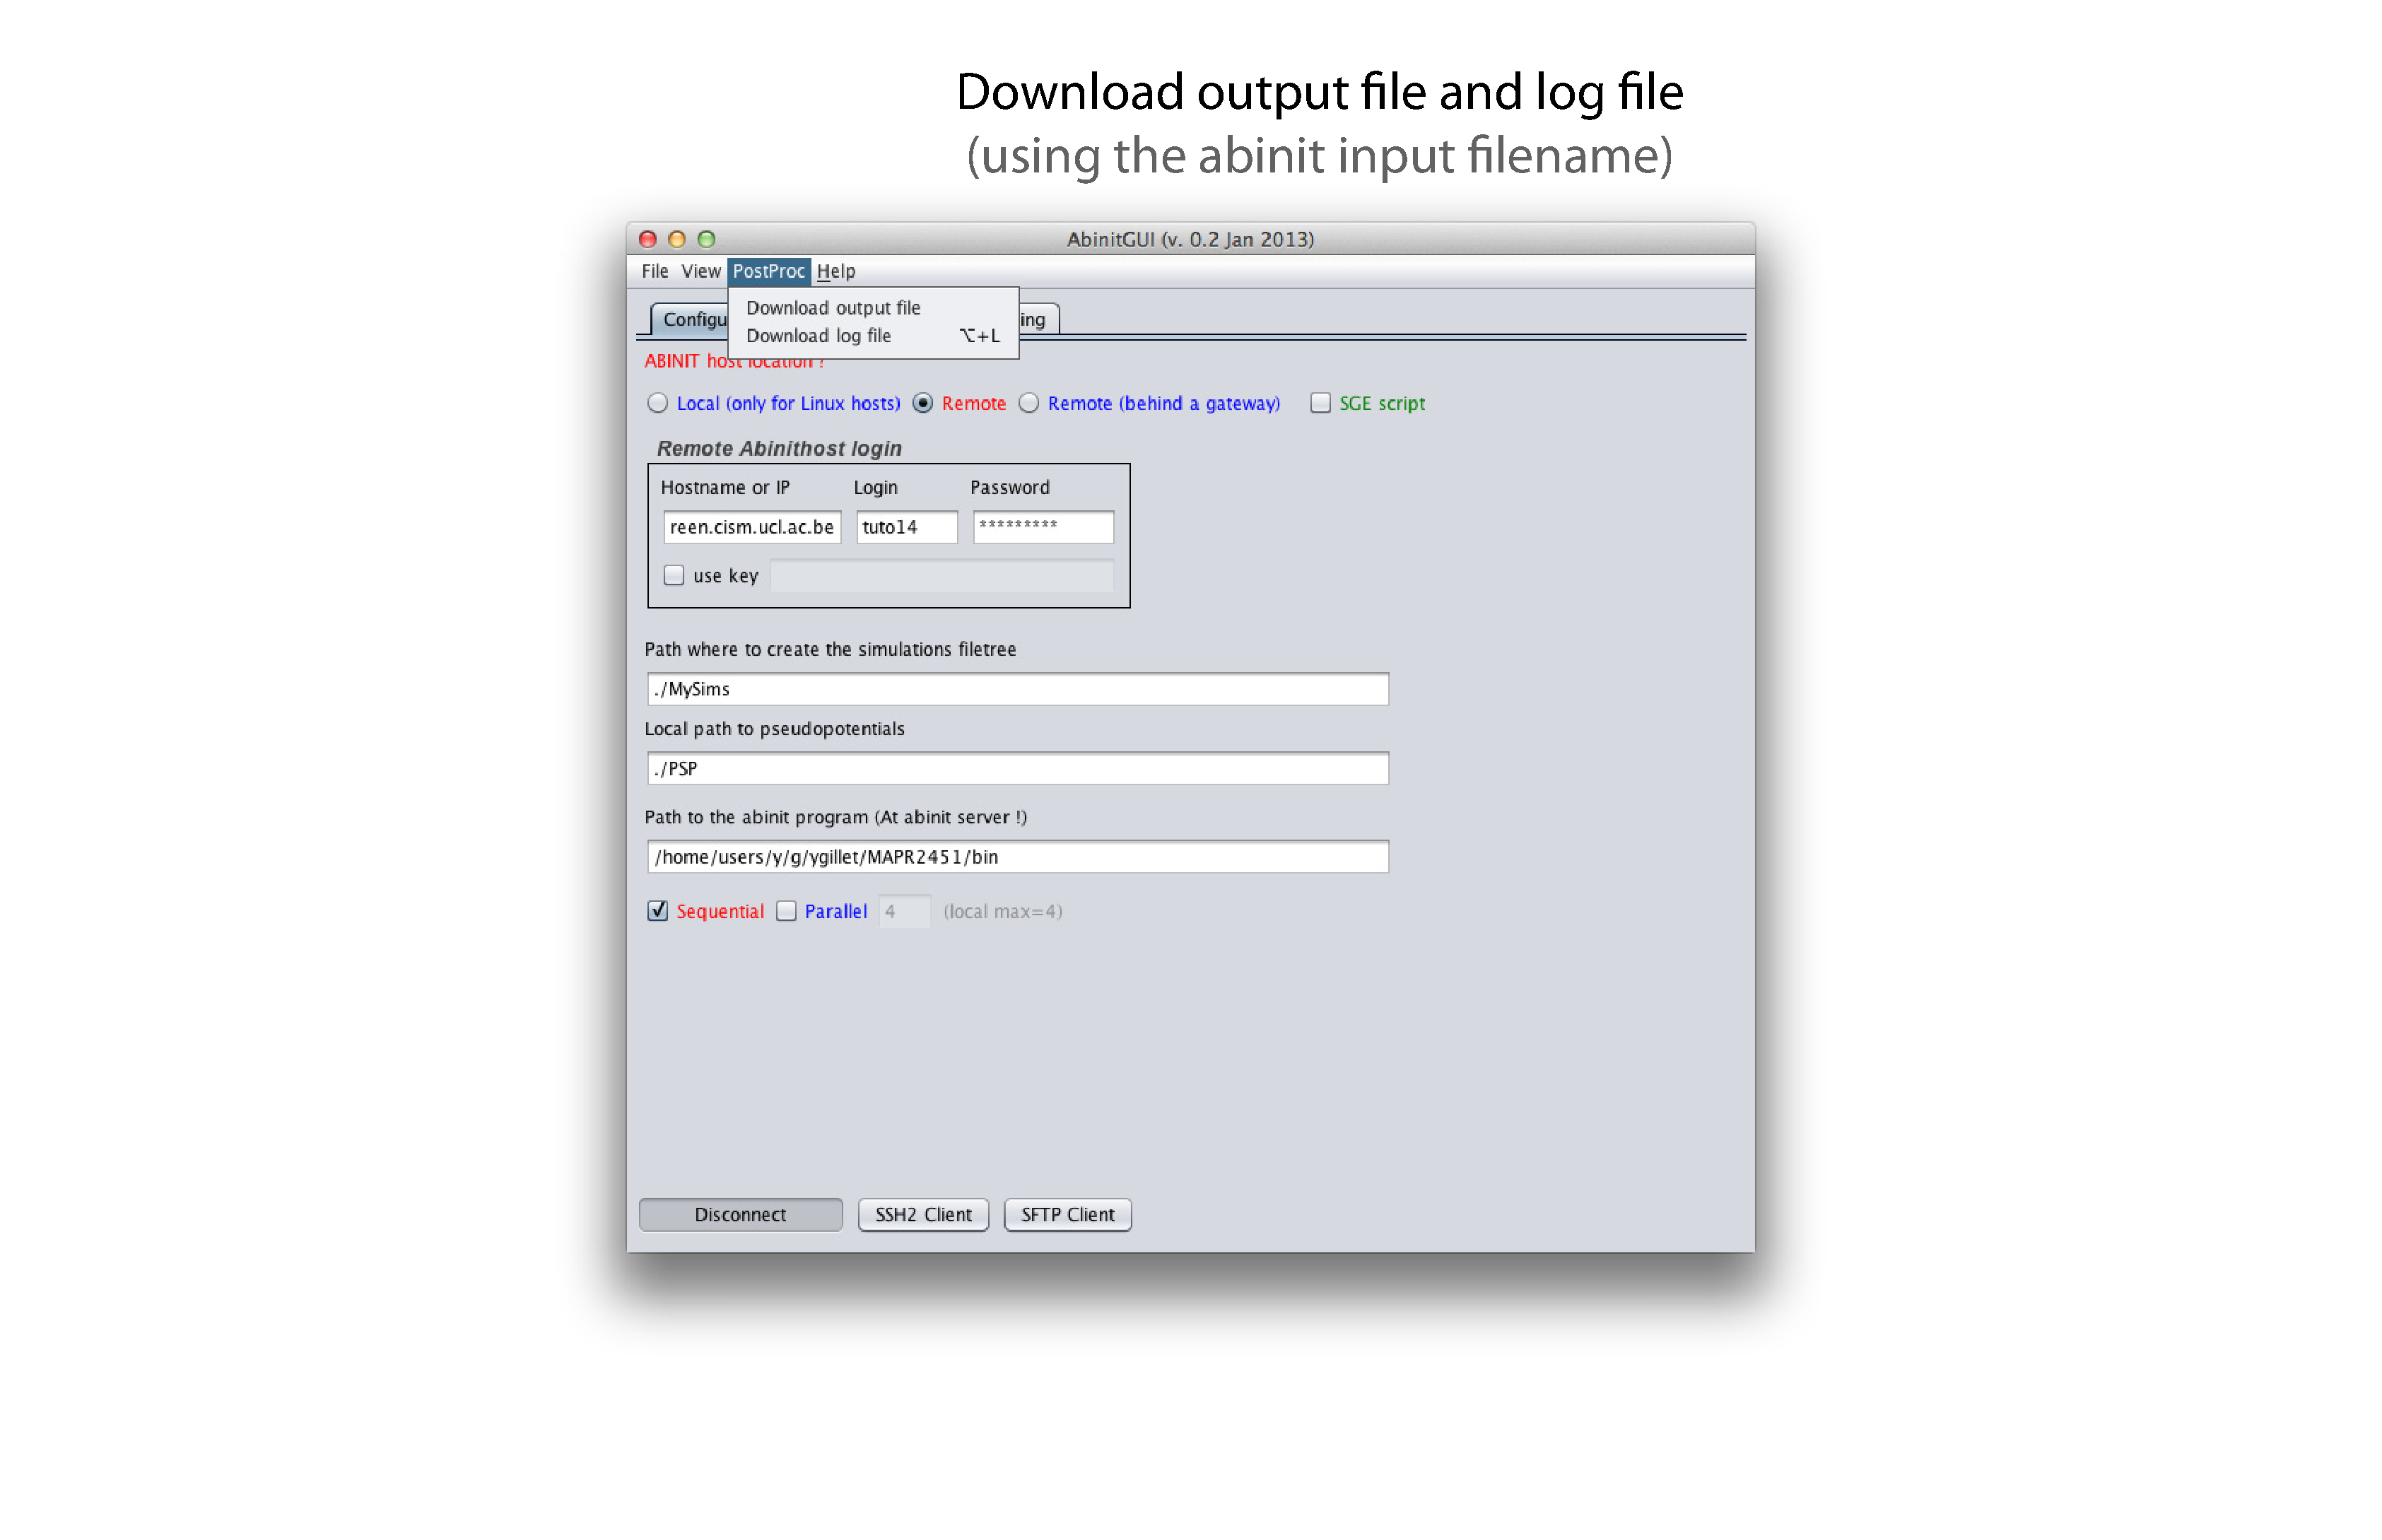
\includegraphics[height=8.25cm]{f6c}\\}
%\only<4>{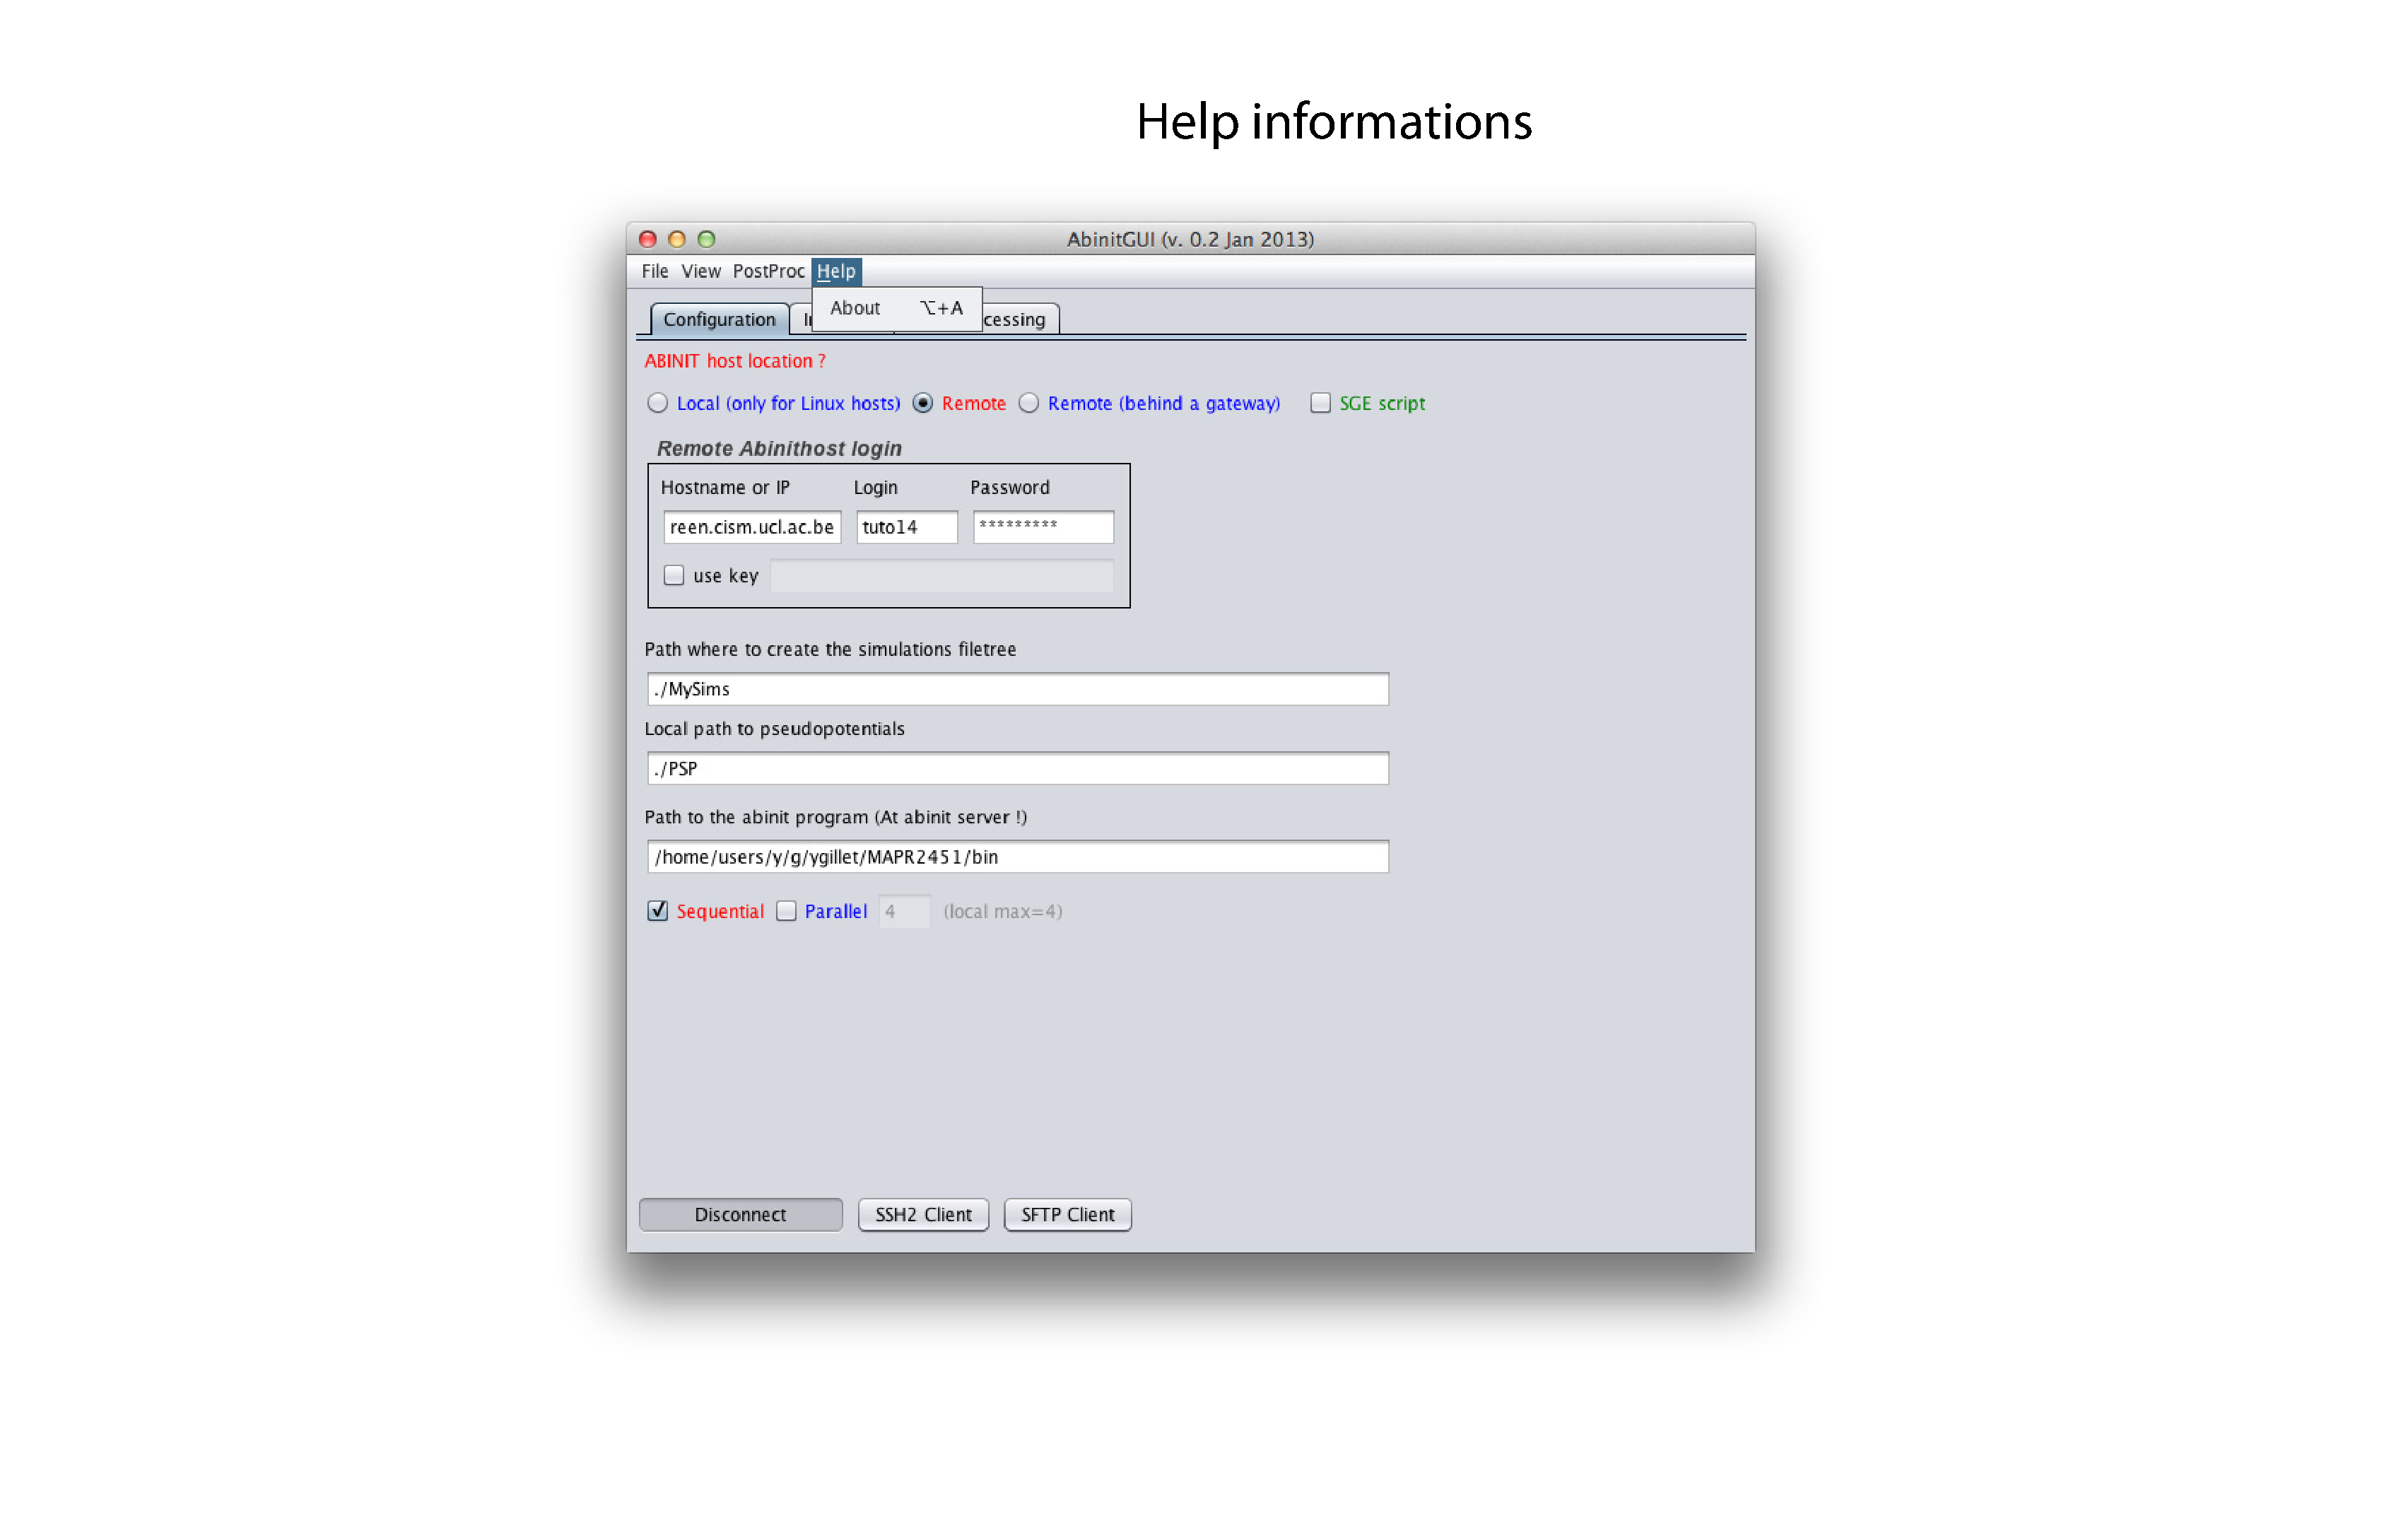
\includegraphics[height=8.25cm]{f6d}\\}
%\end{frame}

%% ----------- F4
\begin{frame}
 \frametitle{Abinit simulation handler}
 \centering
 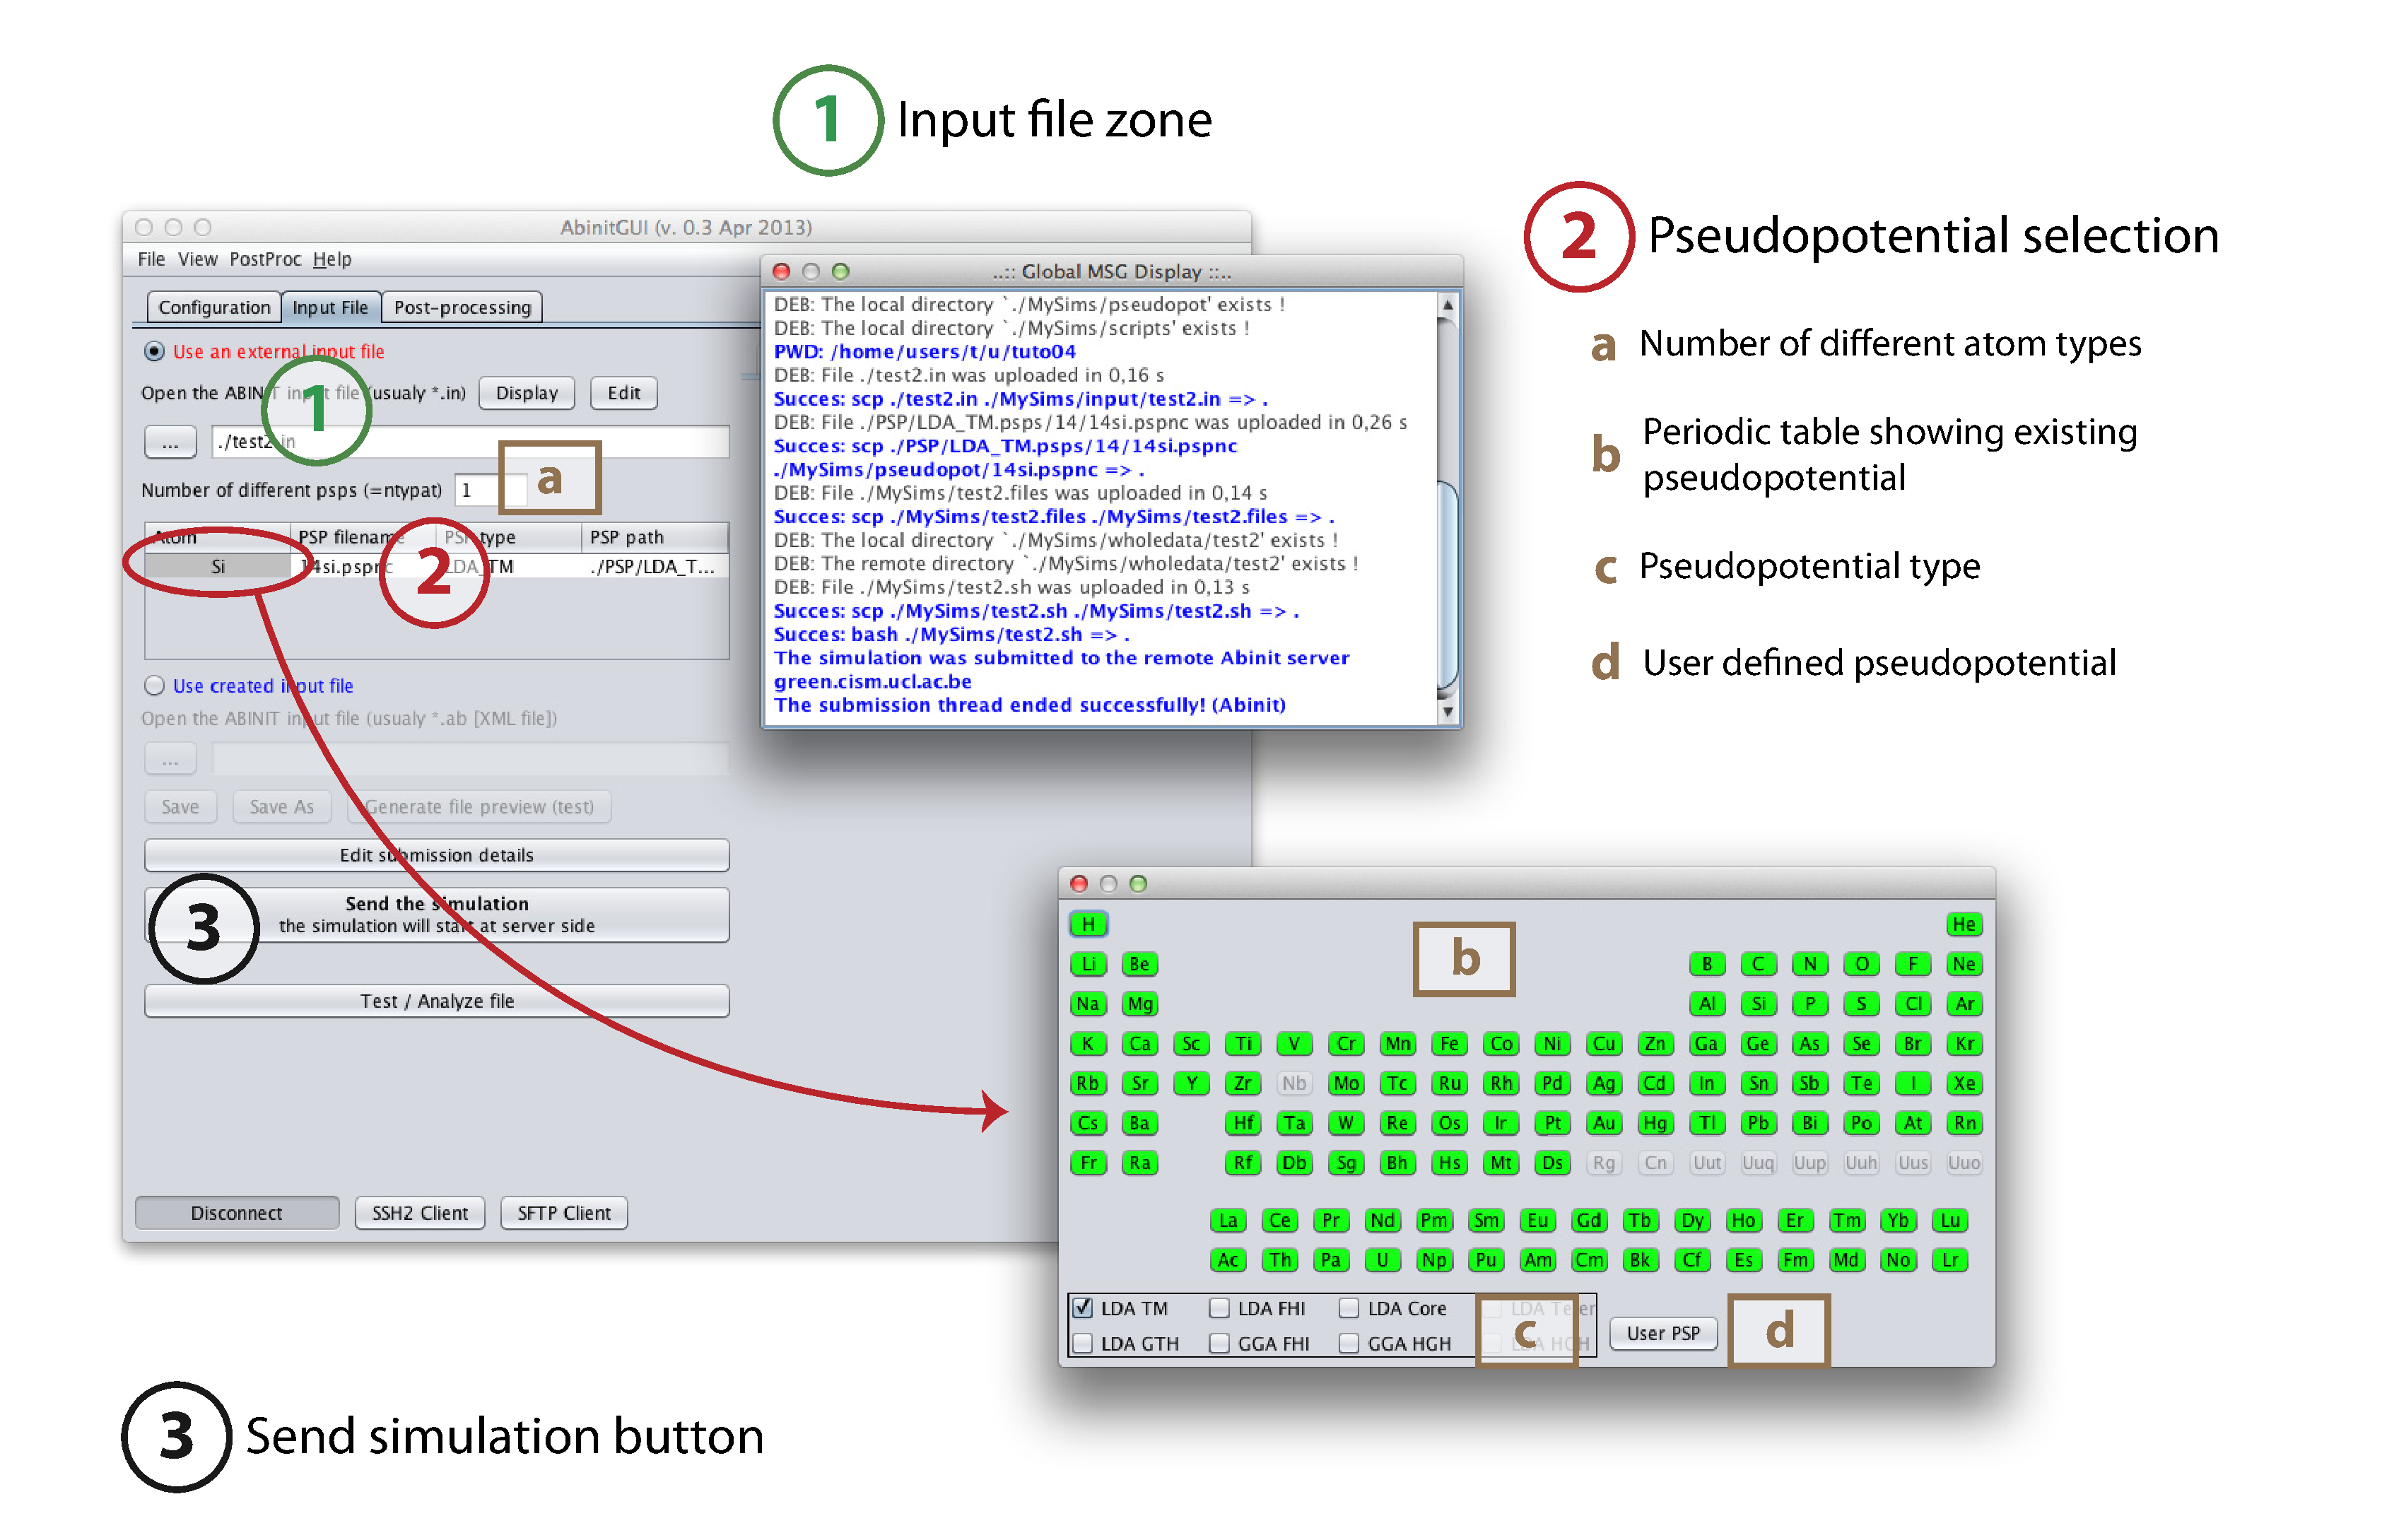
\includegraphics[height=8.25cm]{f2}
\end{frame}

%% ----------- F4 bis
\begin{frame}
 \frametitle{Job submission configuration}
 \centering
 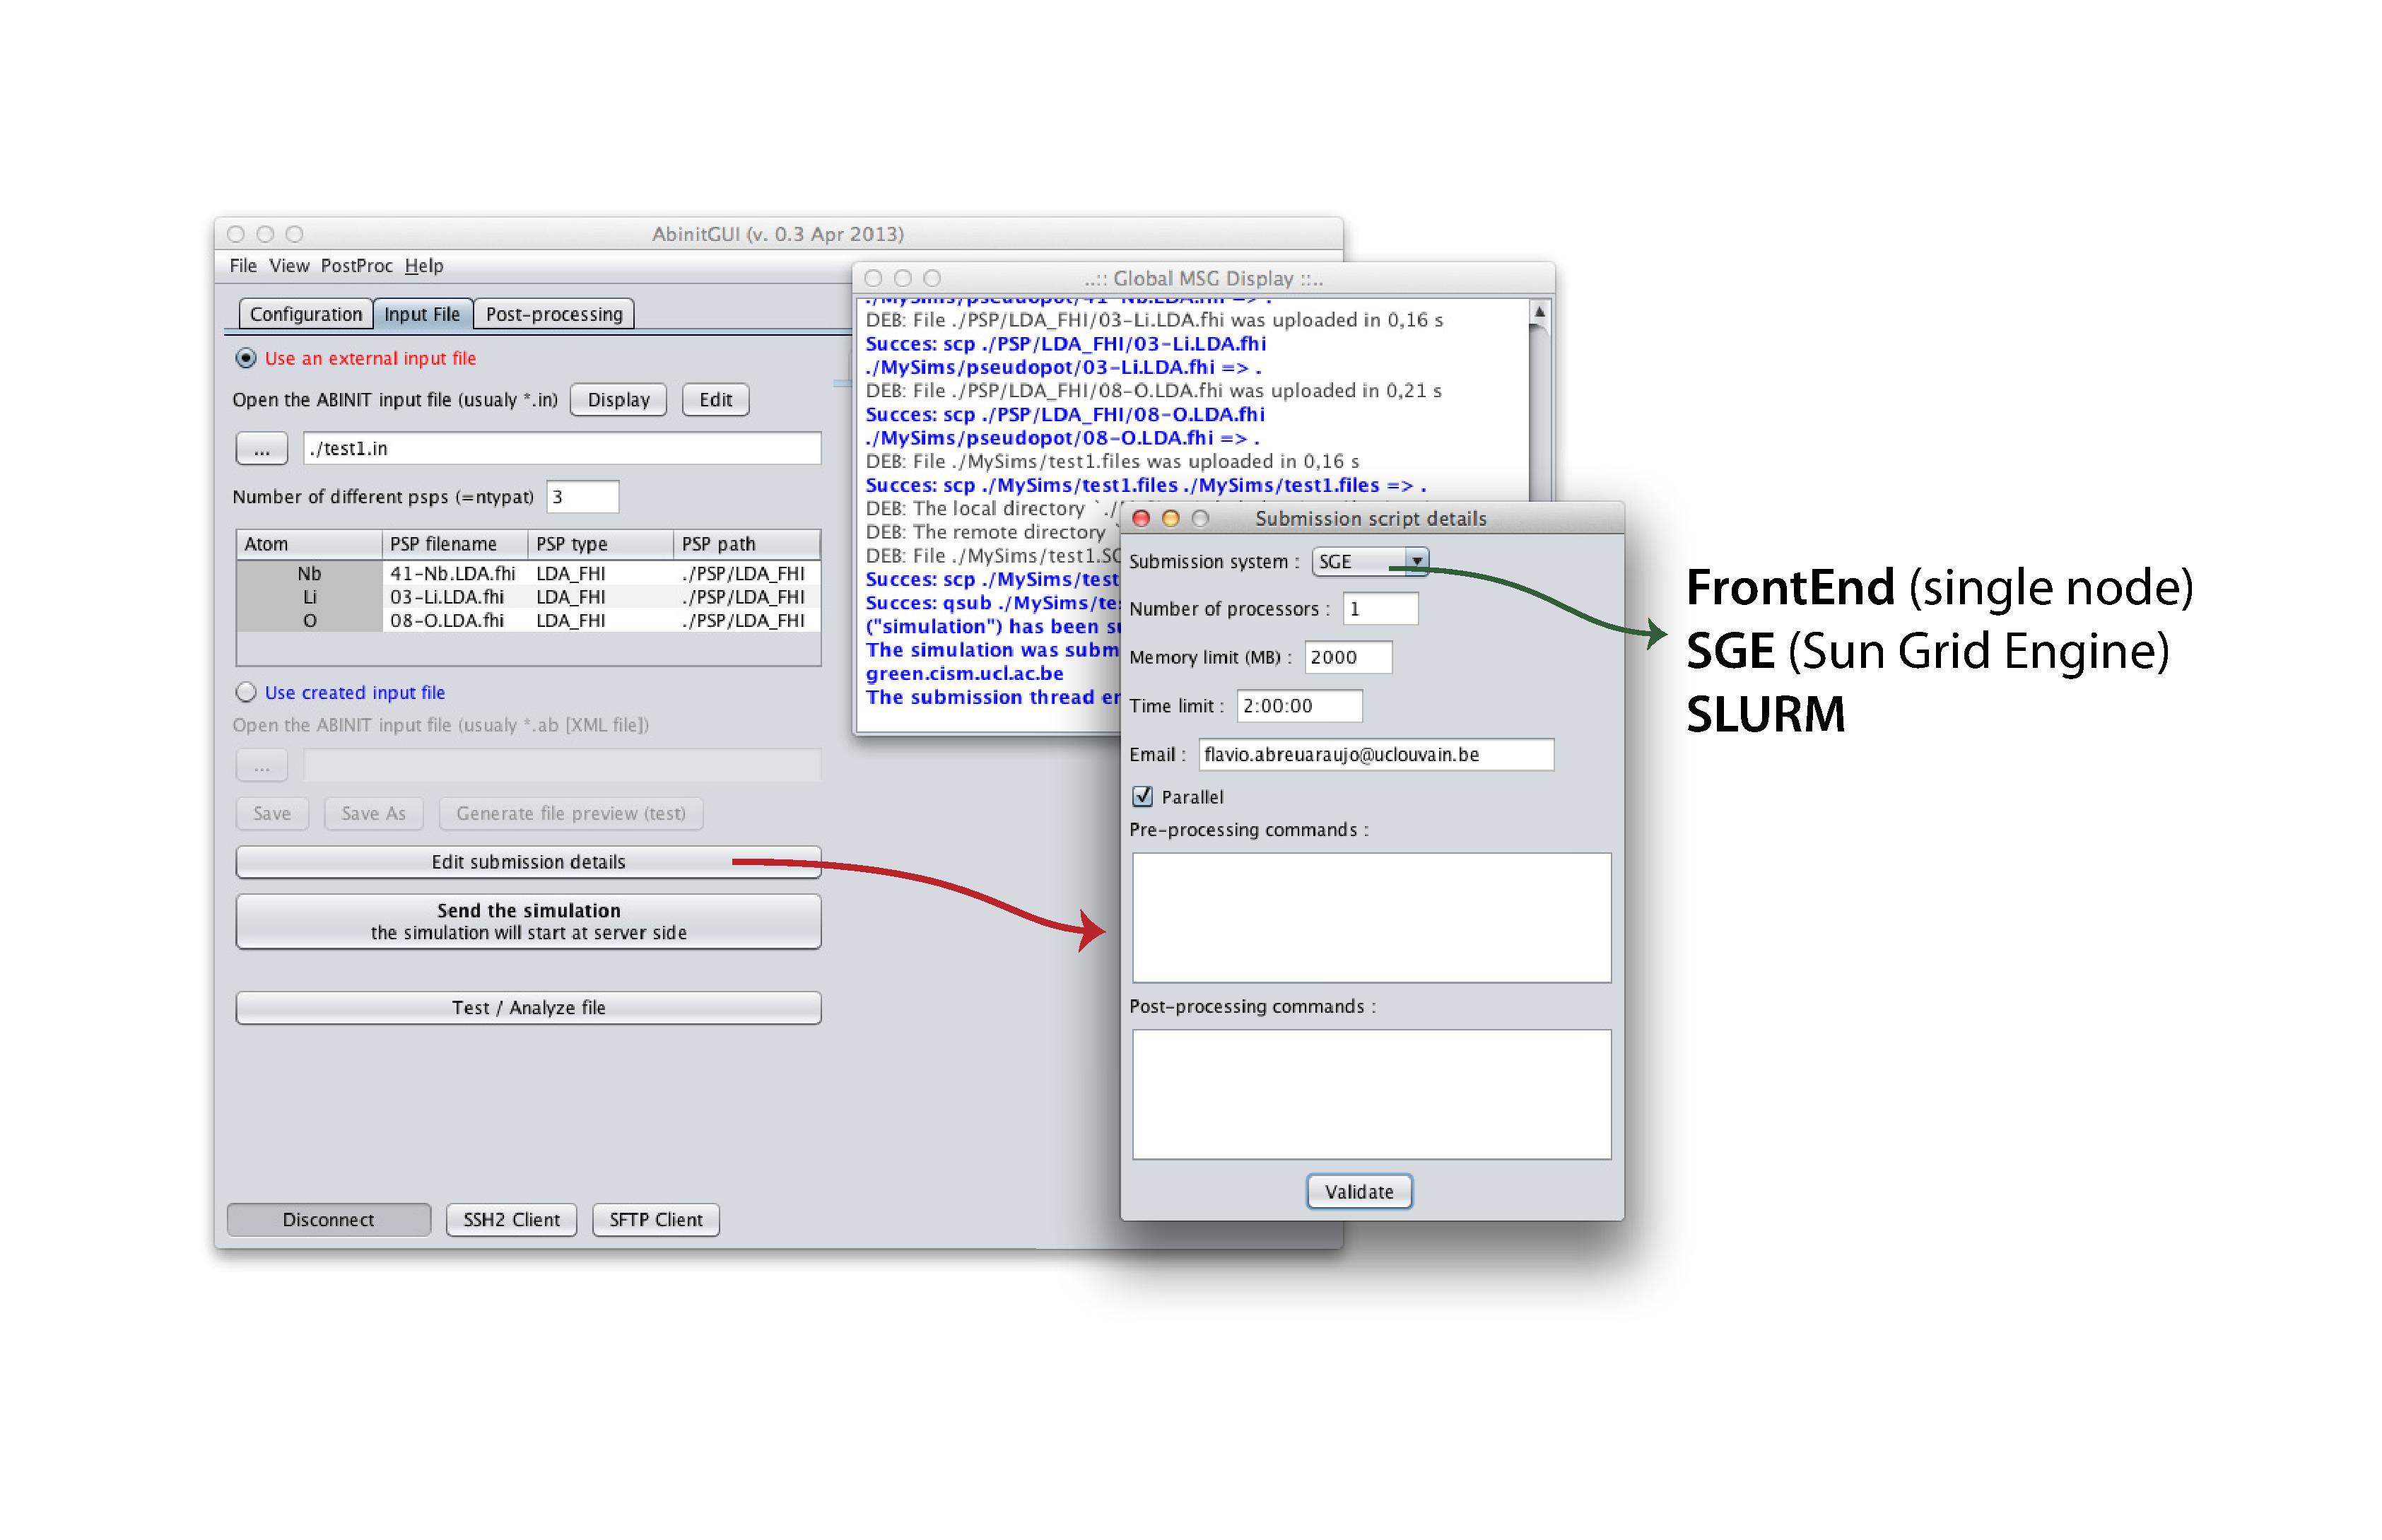
\includegraphics[height=8.25cm]{f2_bis}
\end{frame}

%% ----------- menu3
\begin{frame}
 \frametitle{Output and log files verification}
 \centering
 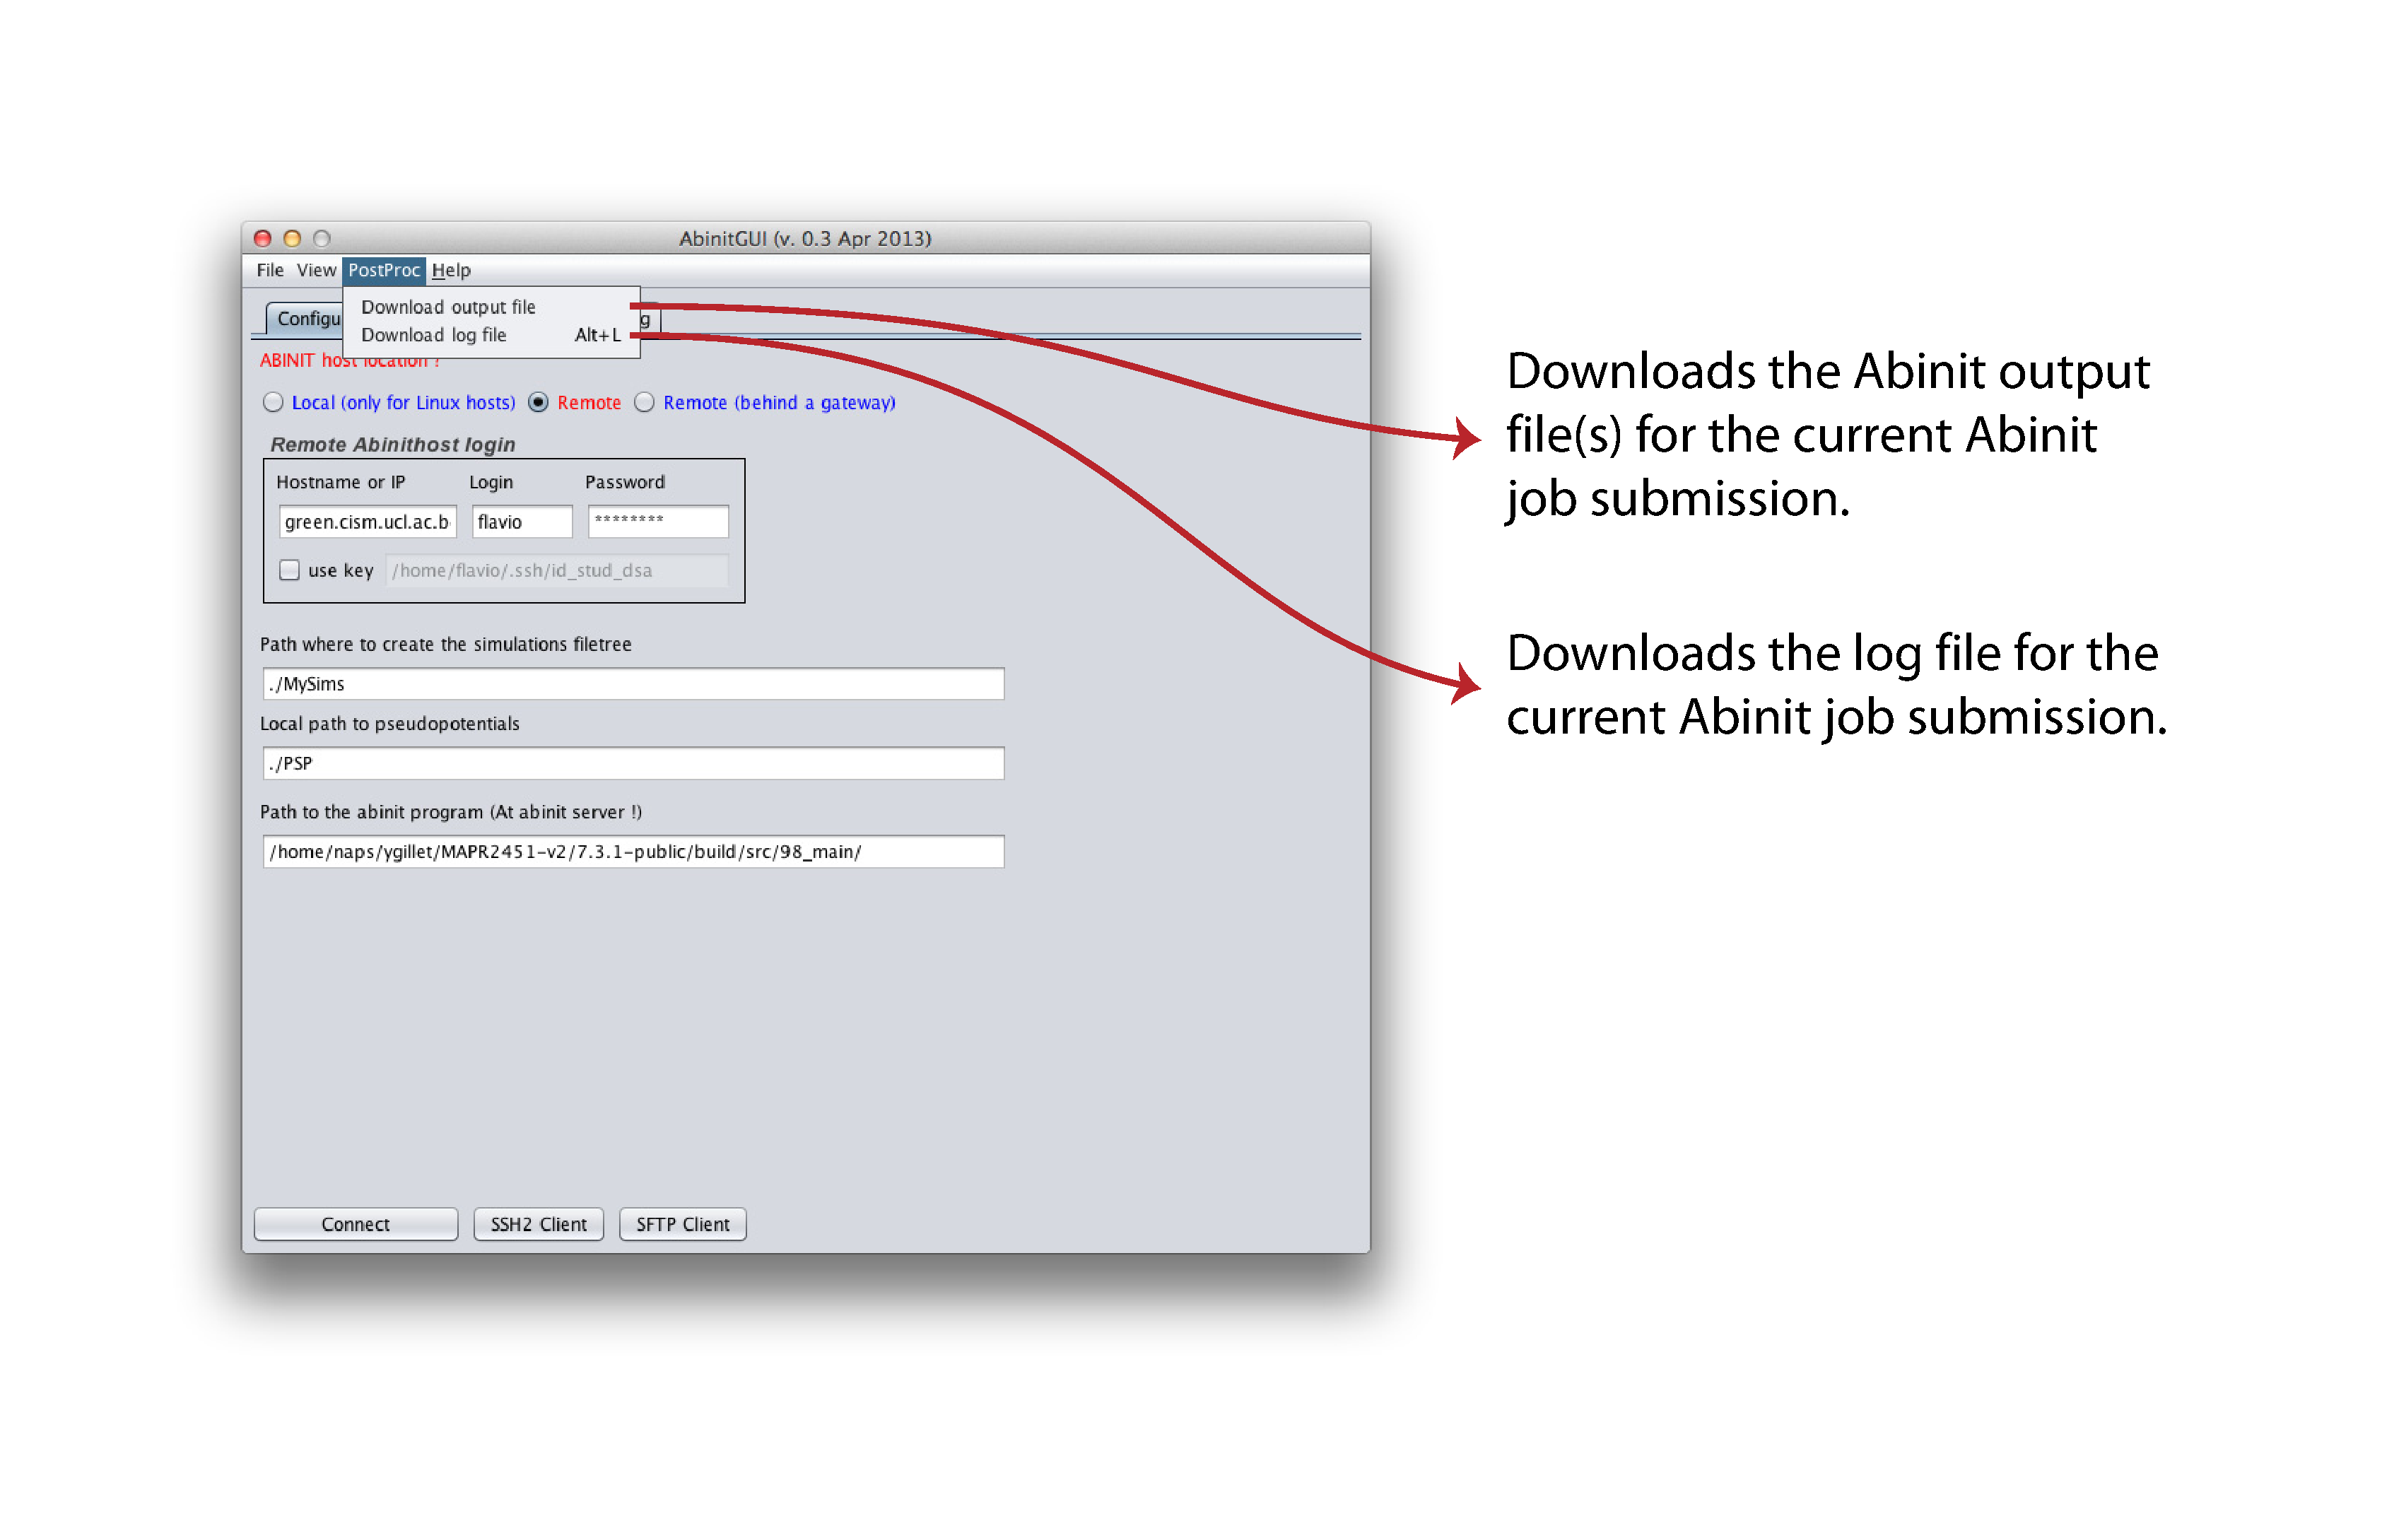
\includegraphics[height=8.25cm]{menu3}
\end{frame}

%%% ----------- menu2
%\begin{frame}
% \frametitle{Menus (2)}
% \centering
% 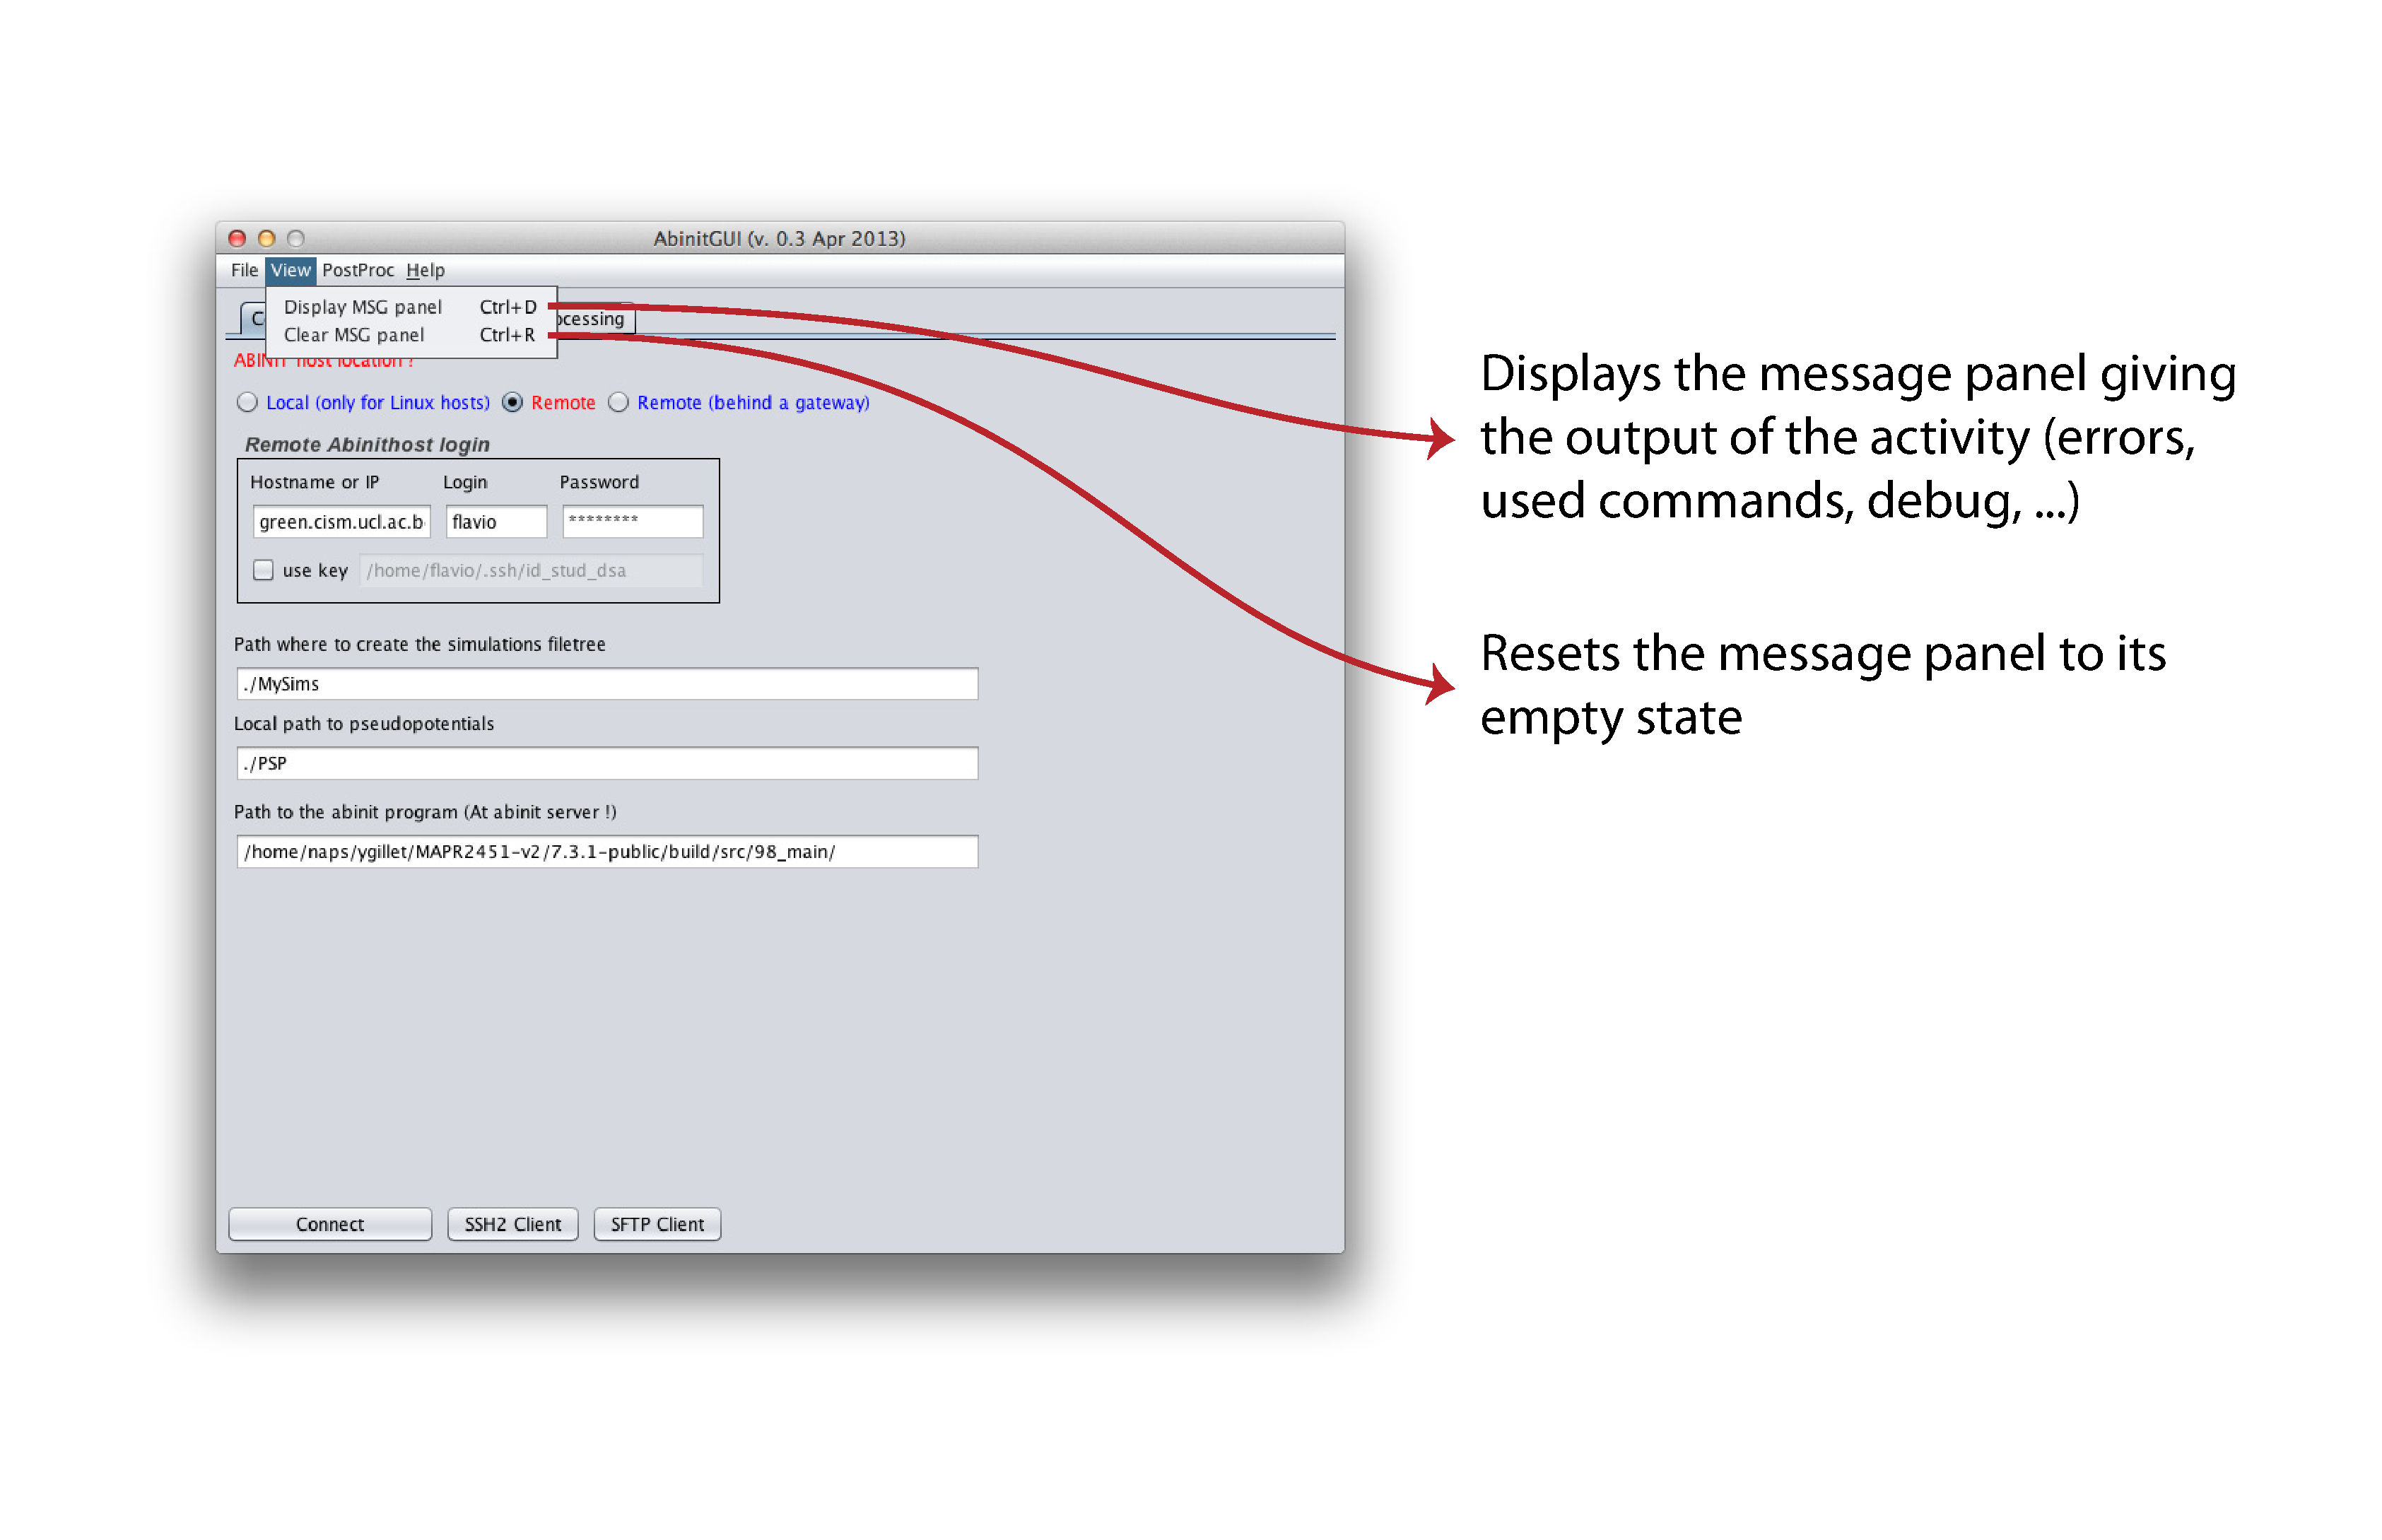
\includegraphics[height=8.25cm]{menu2}
%\end{frame}

%% ----------- F5 bis
\begin{frame}
 \frametitle{Abinit input variables help}
 \centering
 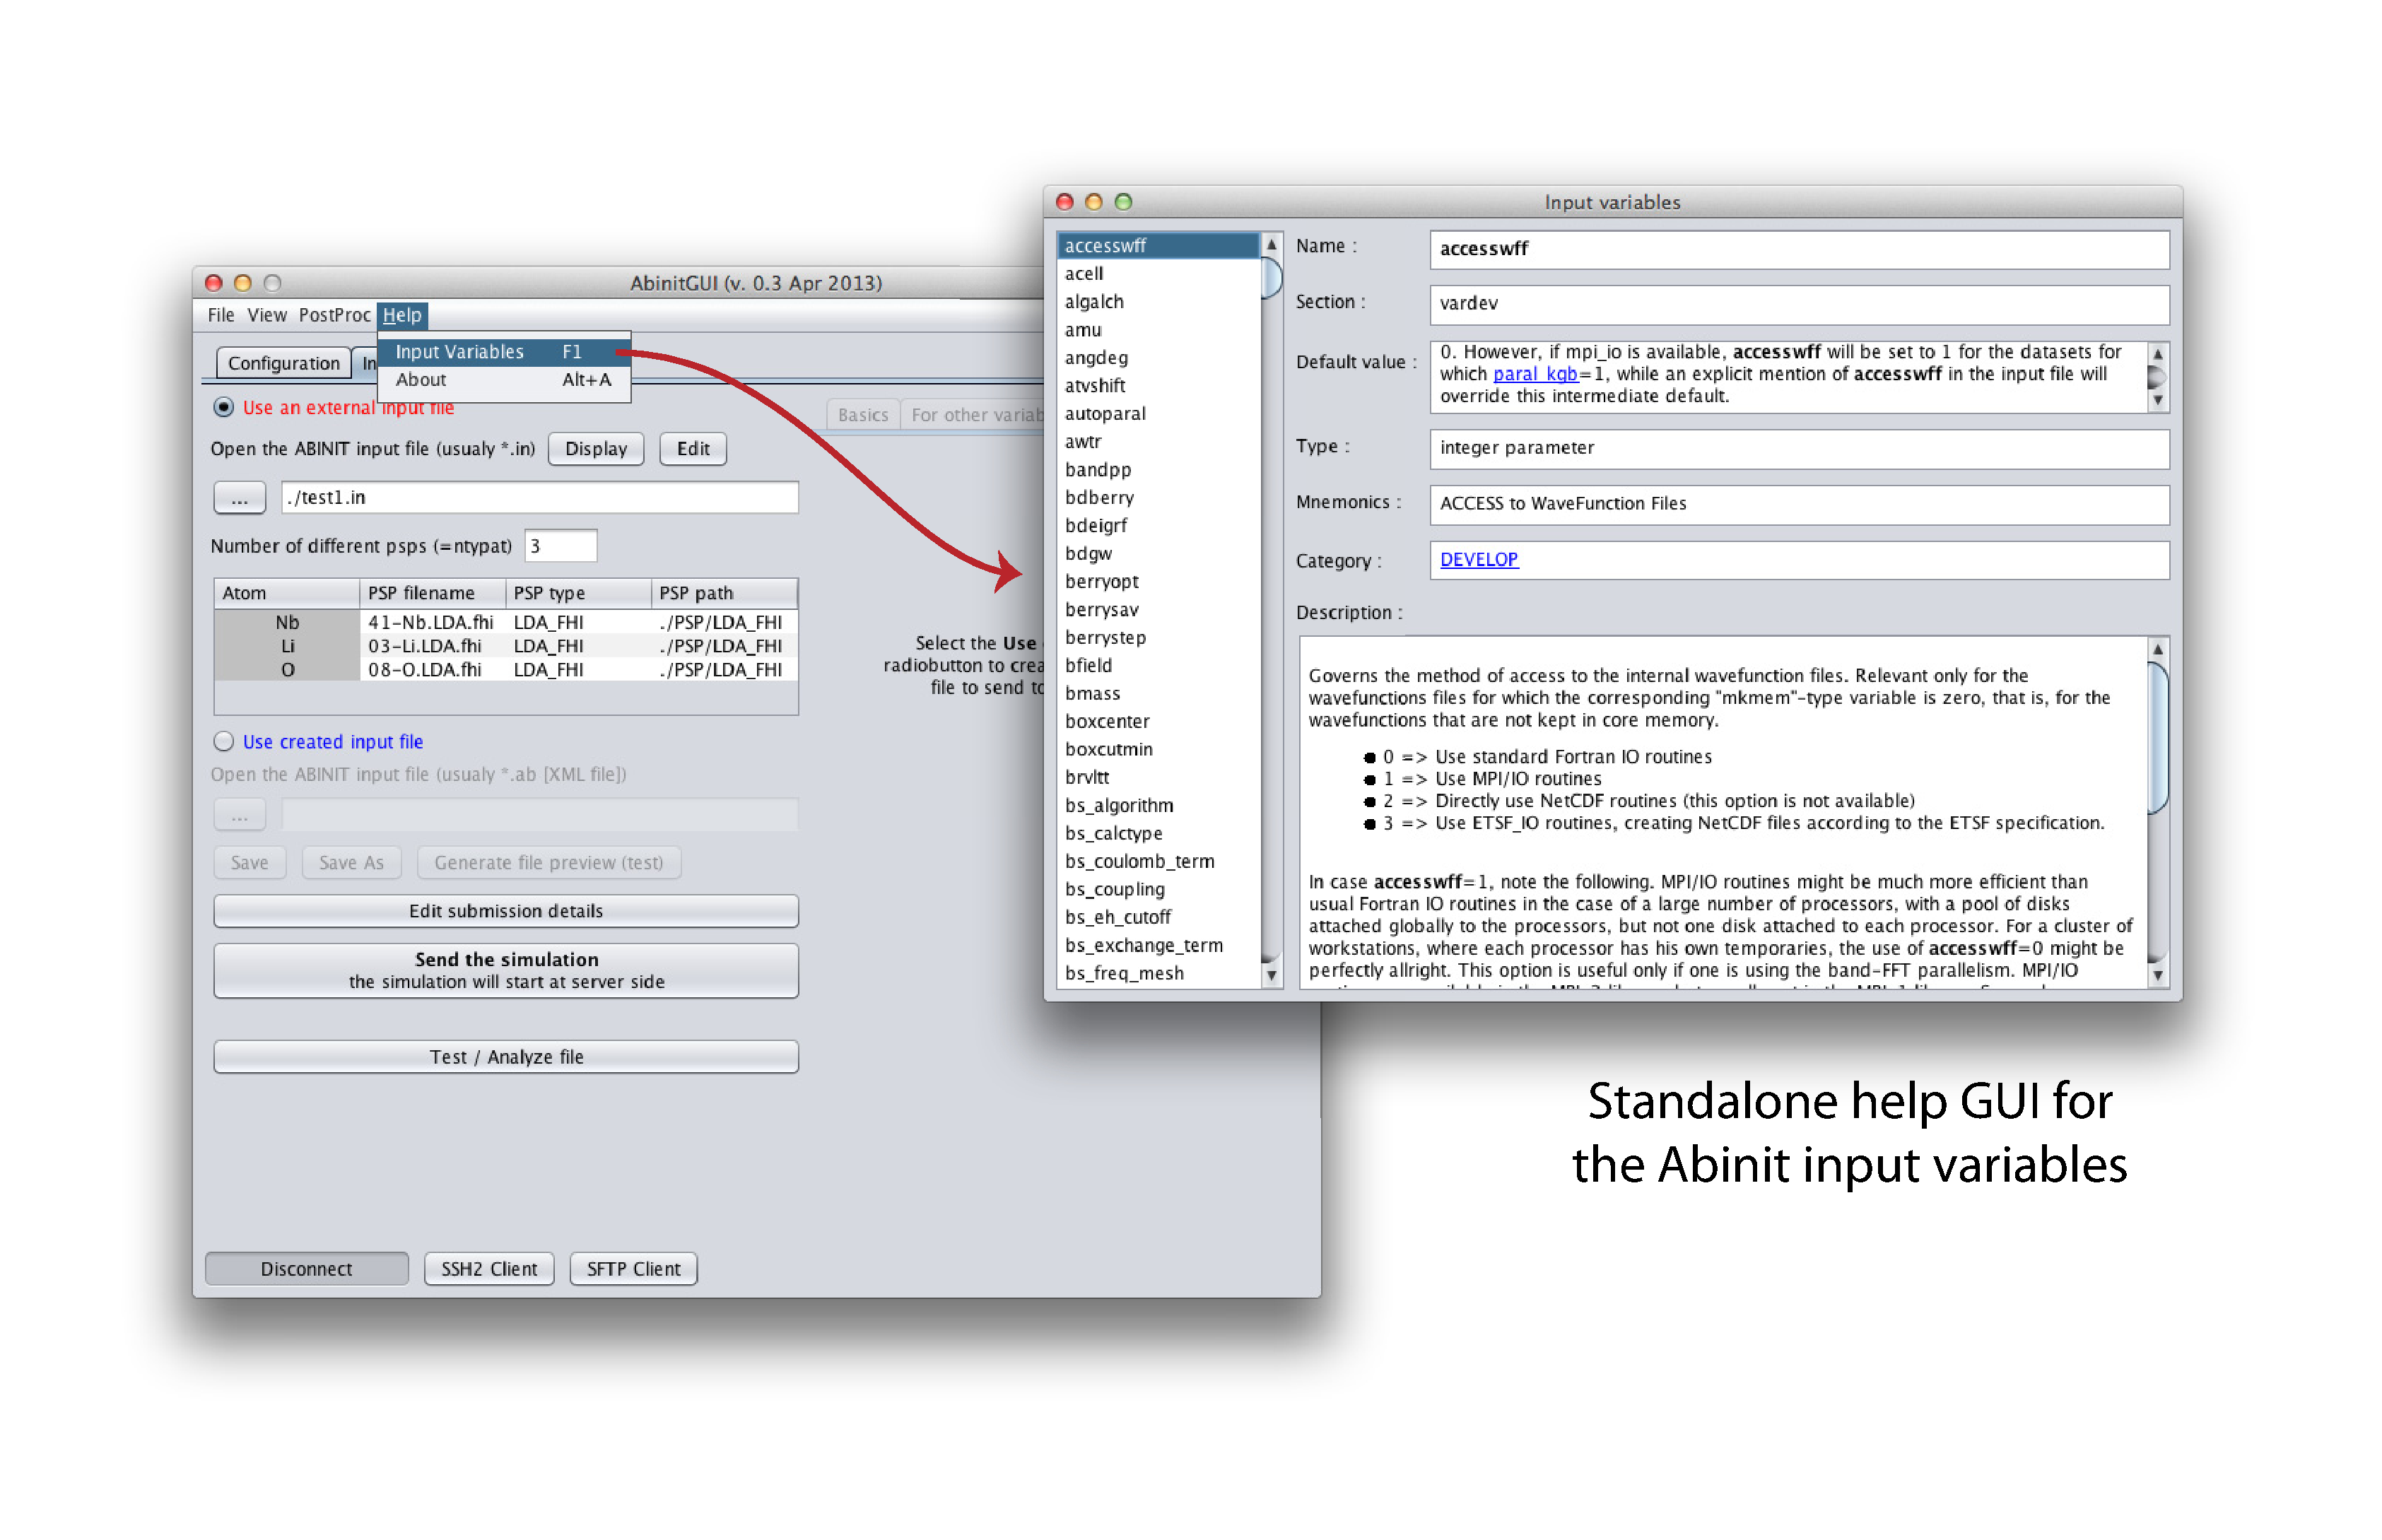
\includegraphics[height=8.25cm]{f3_bis}
\end{frame}

%% ----------- F5
\begin{frame}
 \frametitle{Geometry visualisation with Jmol}
 \centering
 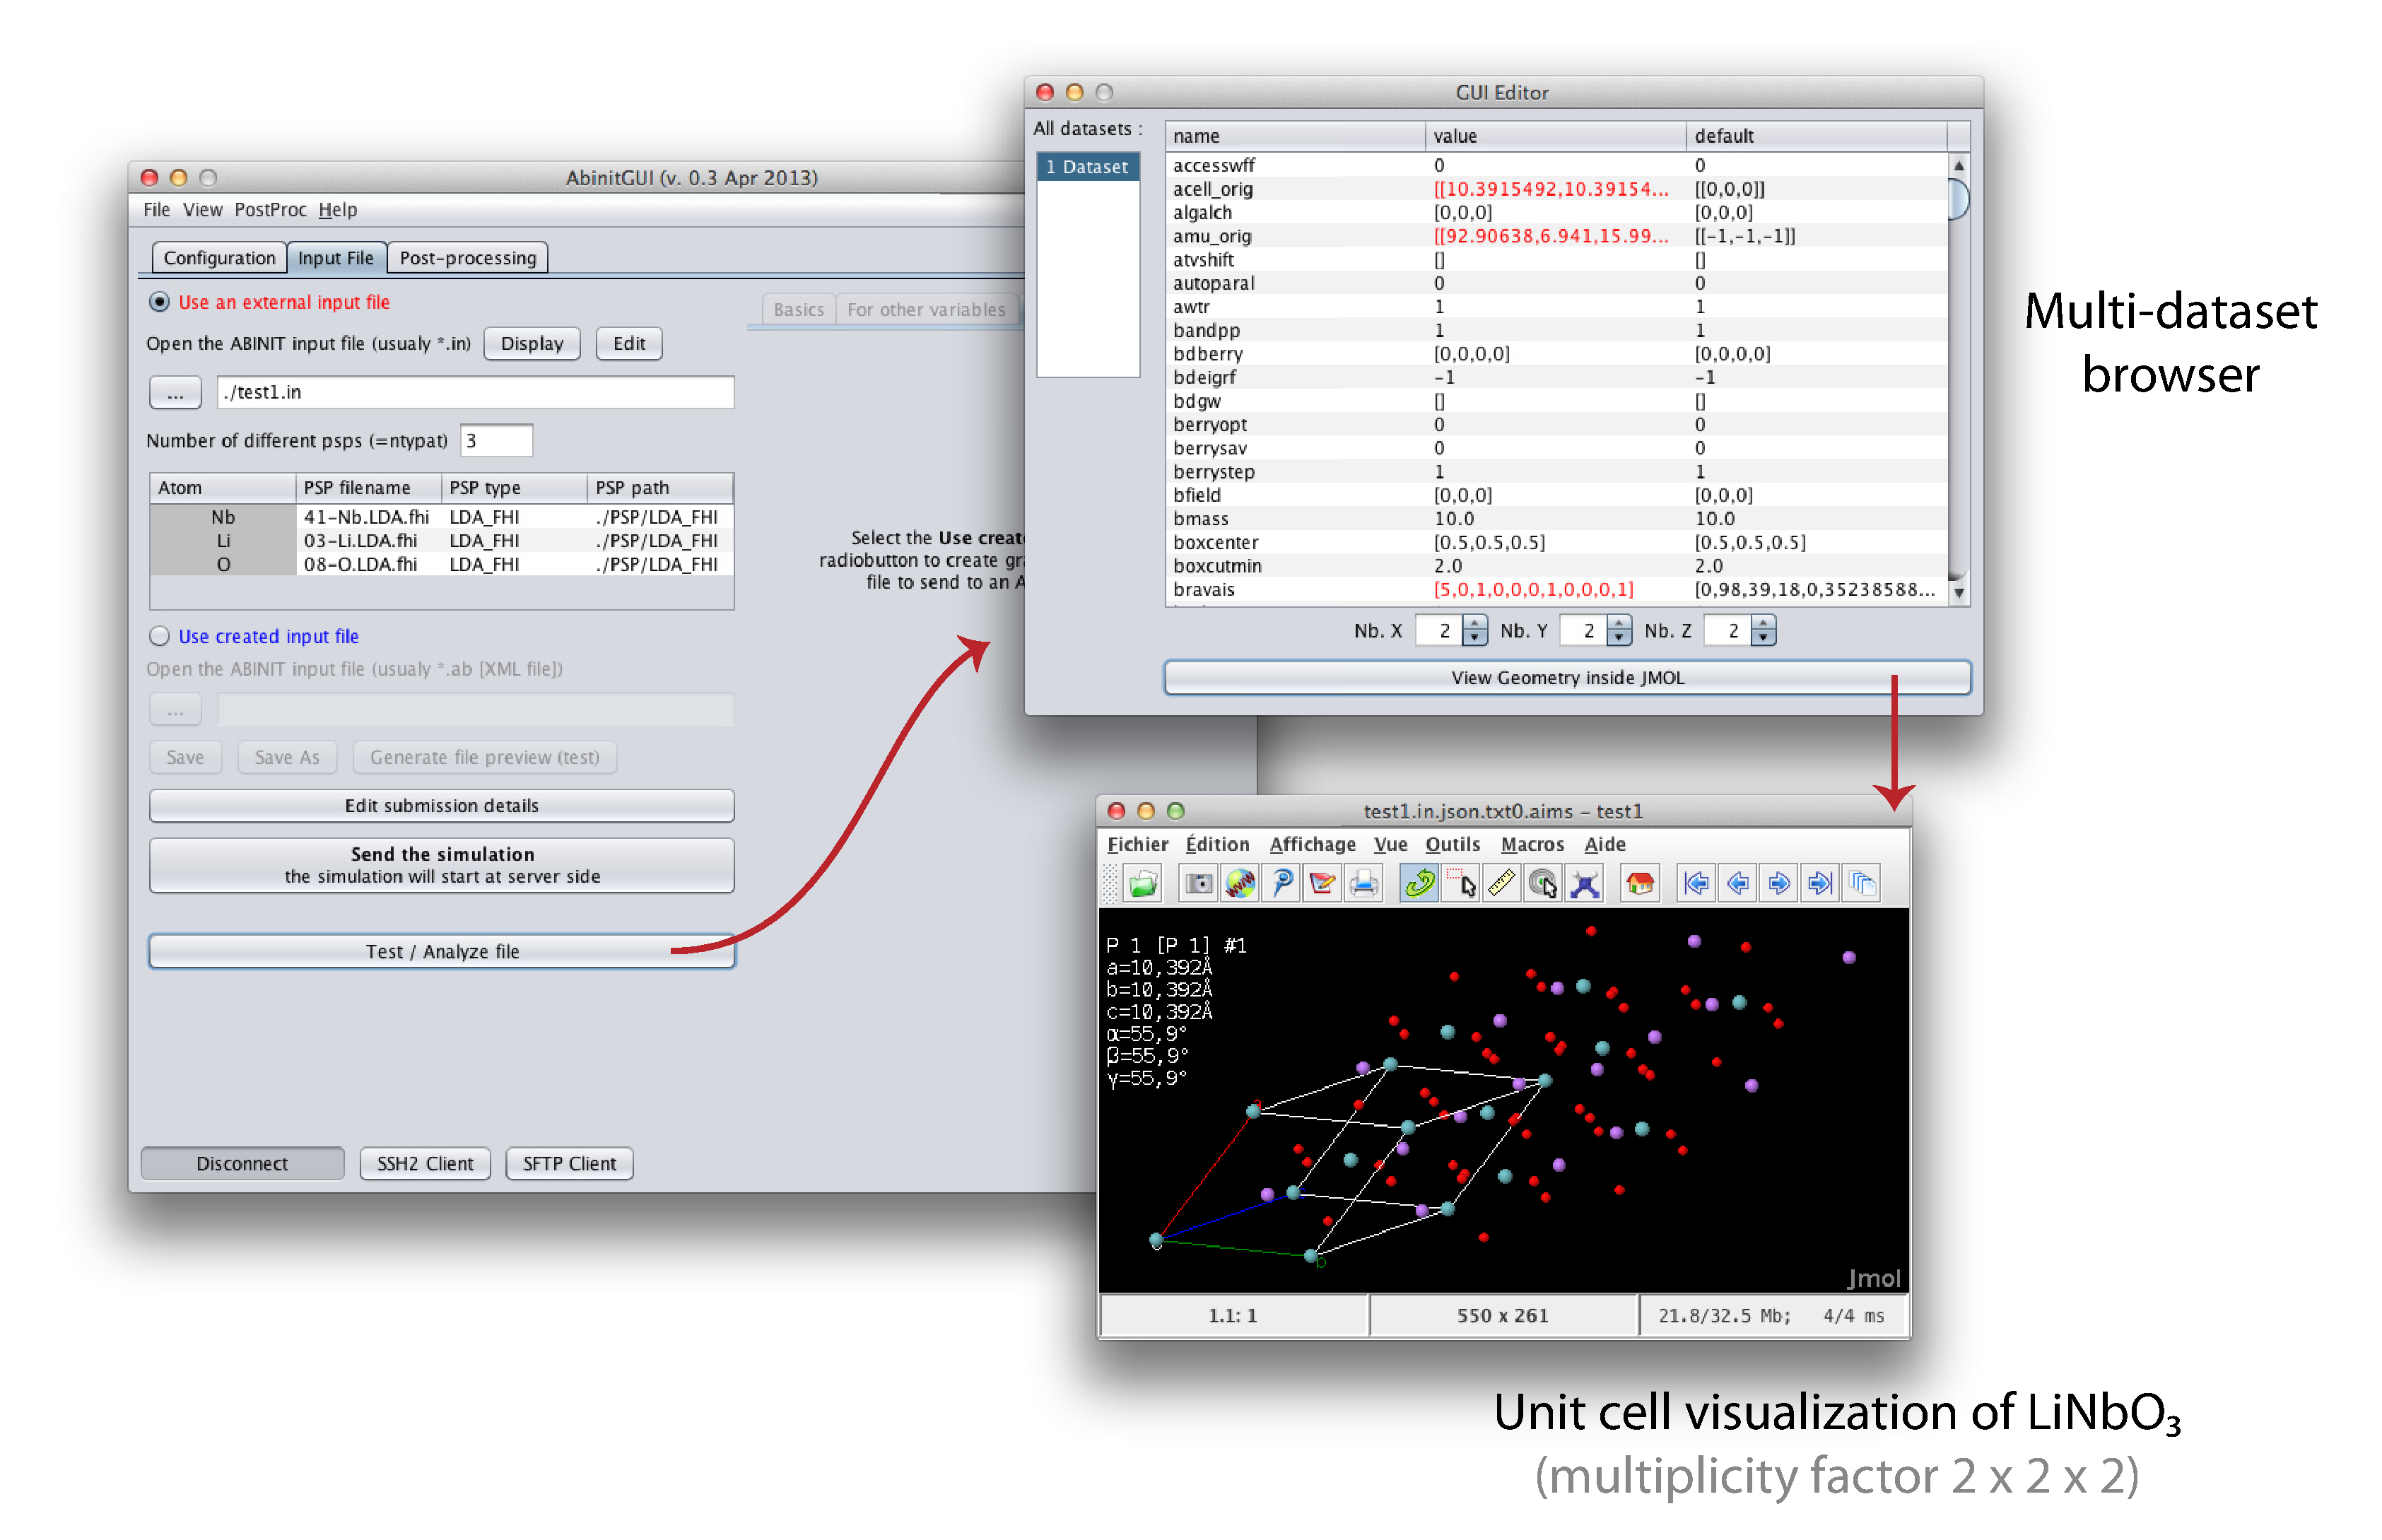
\includegraphics[height=8.25cm]{f3}
 \begin{textblock*}{8cm}(4.1cm,5.4cm)
  \begin{figure}
  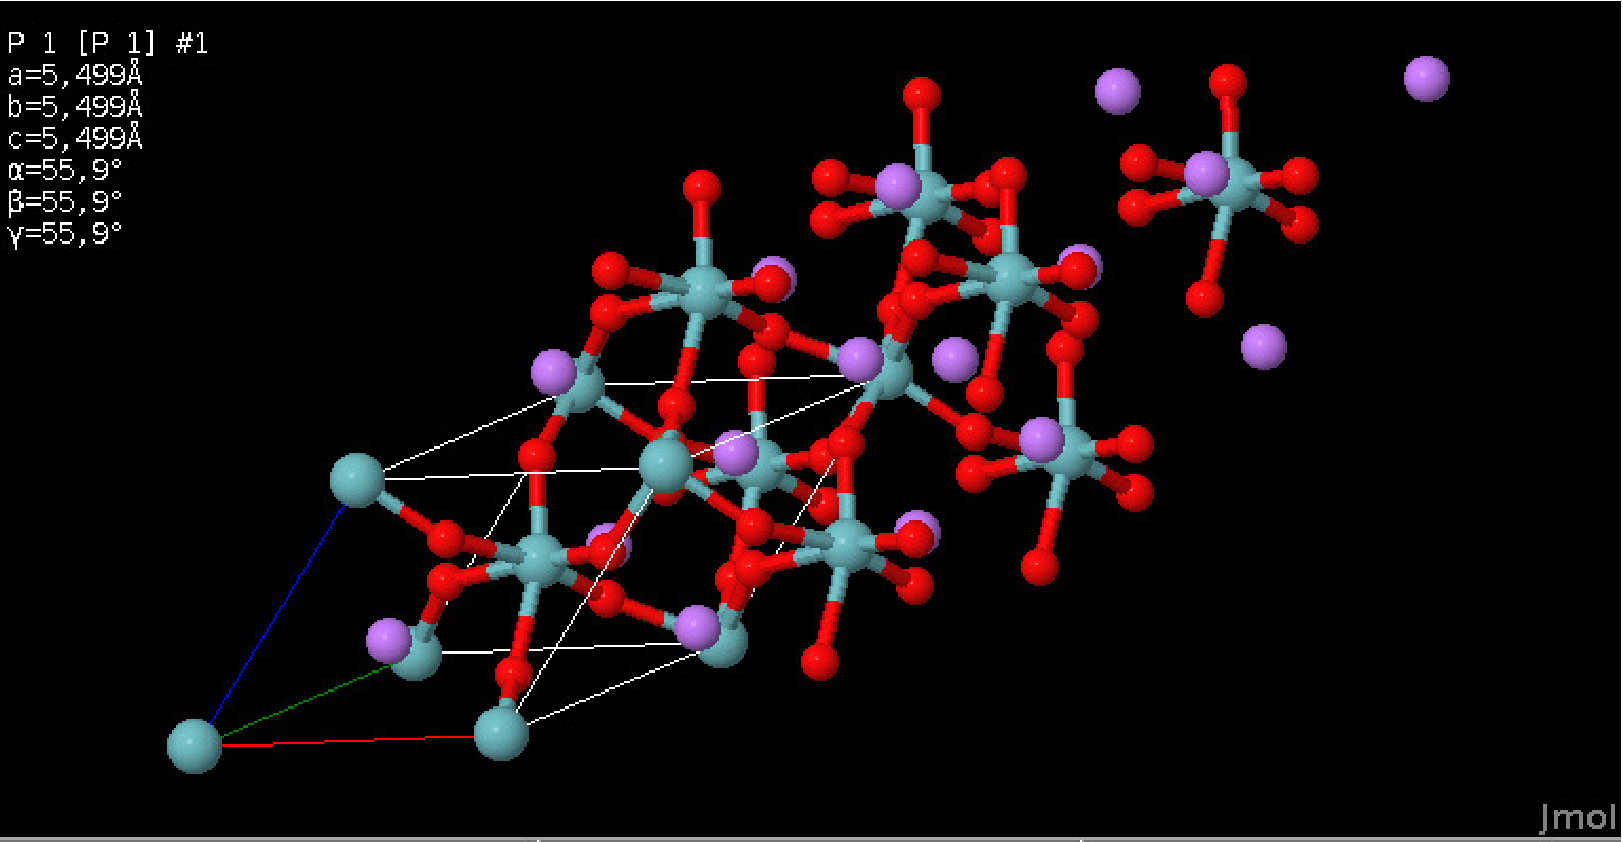
\includegraphics[height=2cm,width=4.3cm]{image-linux}
  \end{figure}
 \end{textblock*}

\end{frame}

%% ----------- F7
\begin{frame}
 \frametitle{Post-processing}
\centering
\only<1>{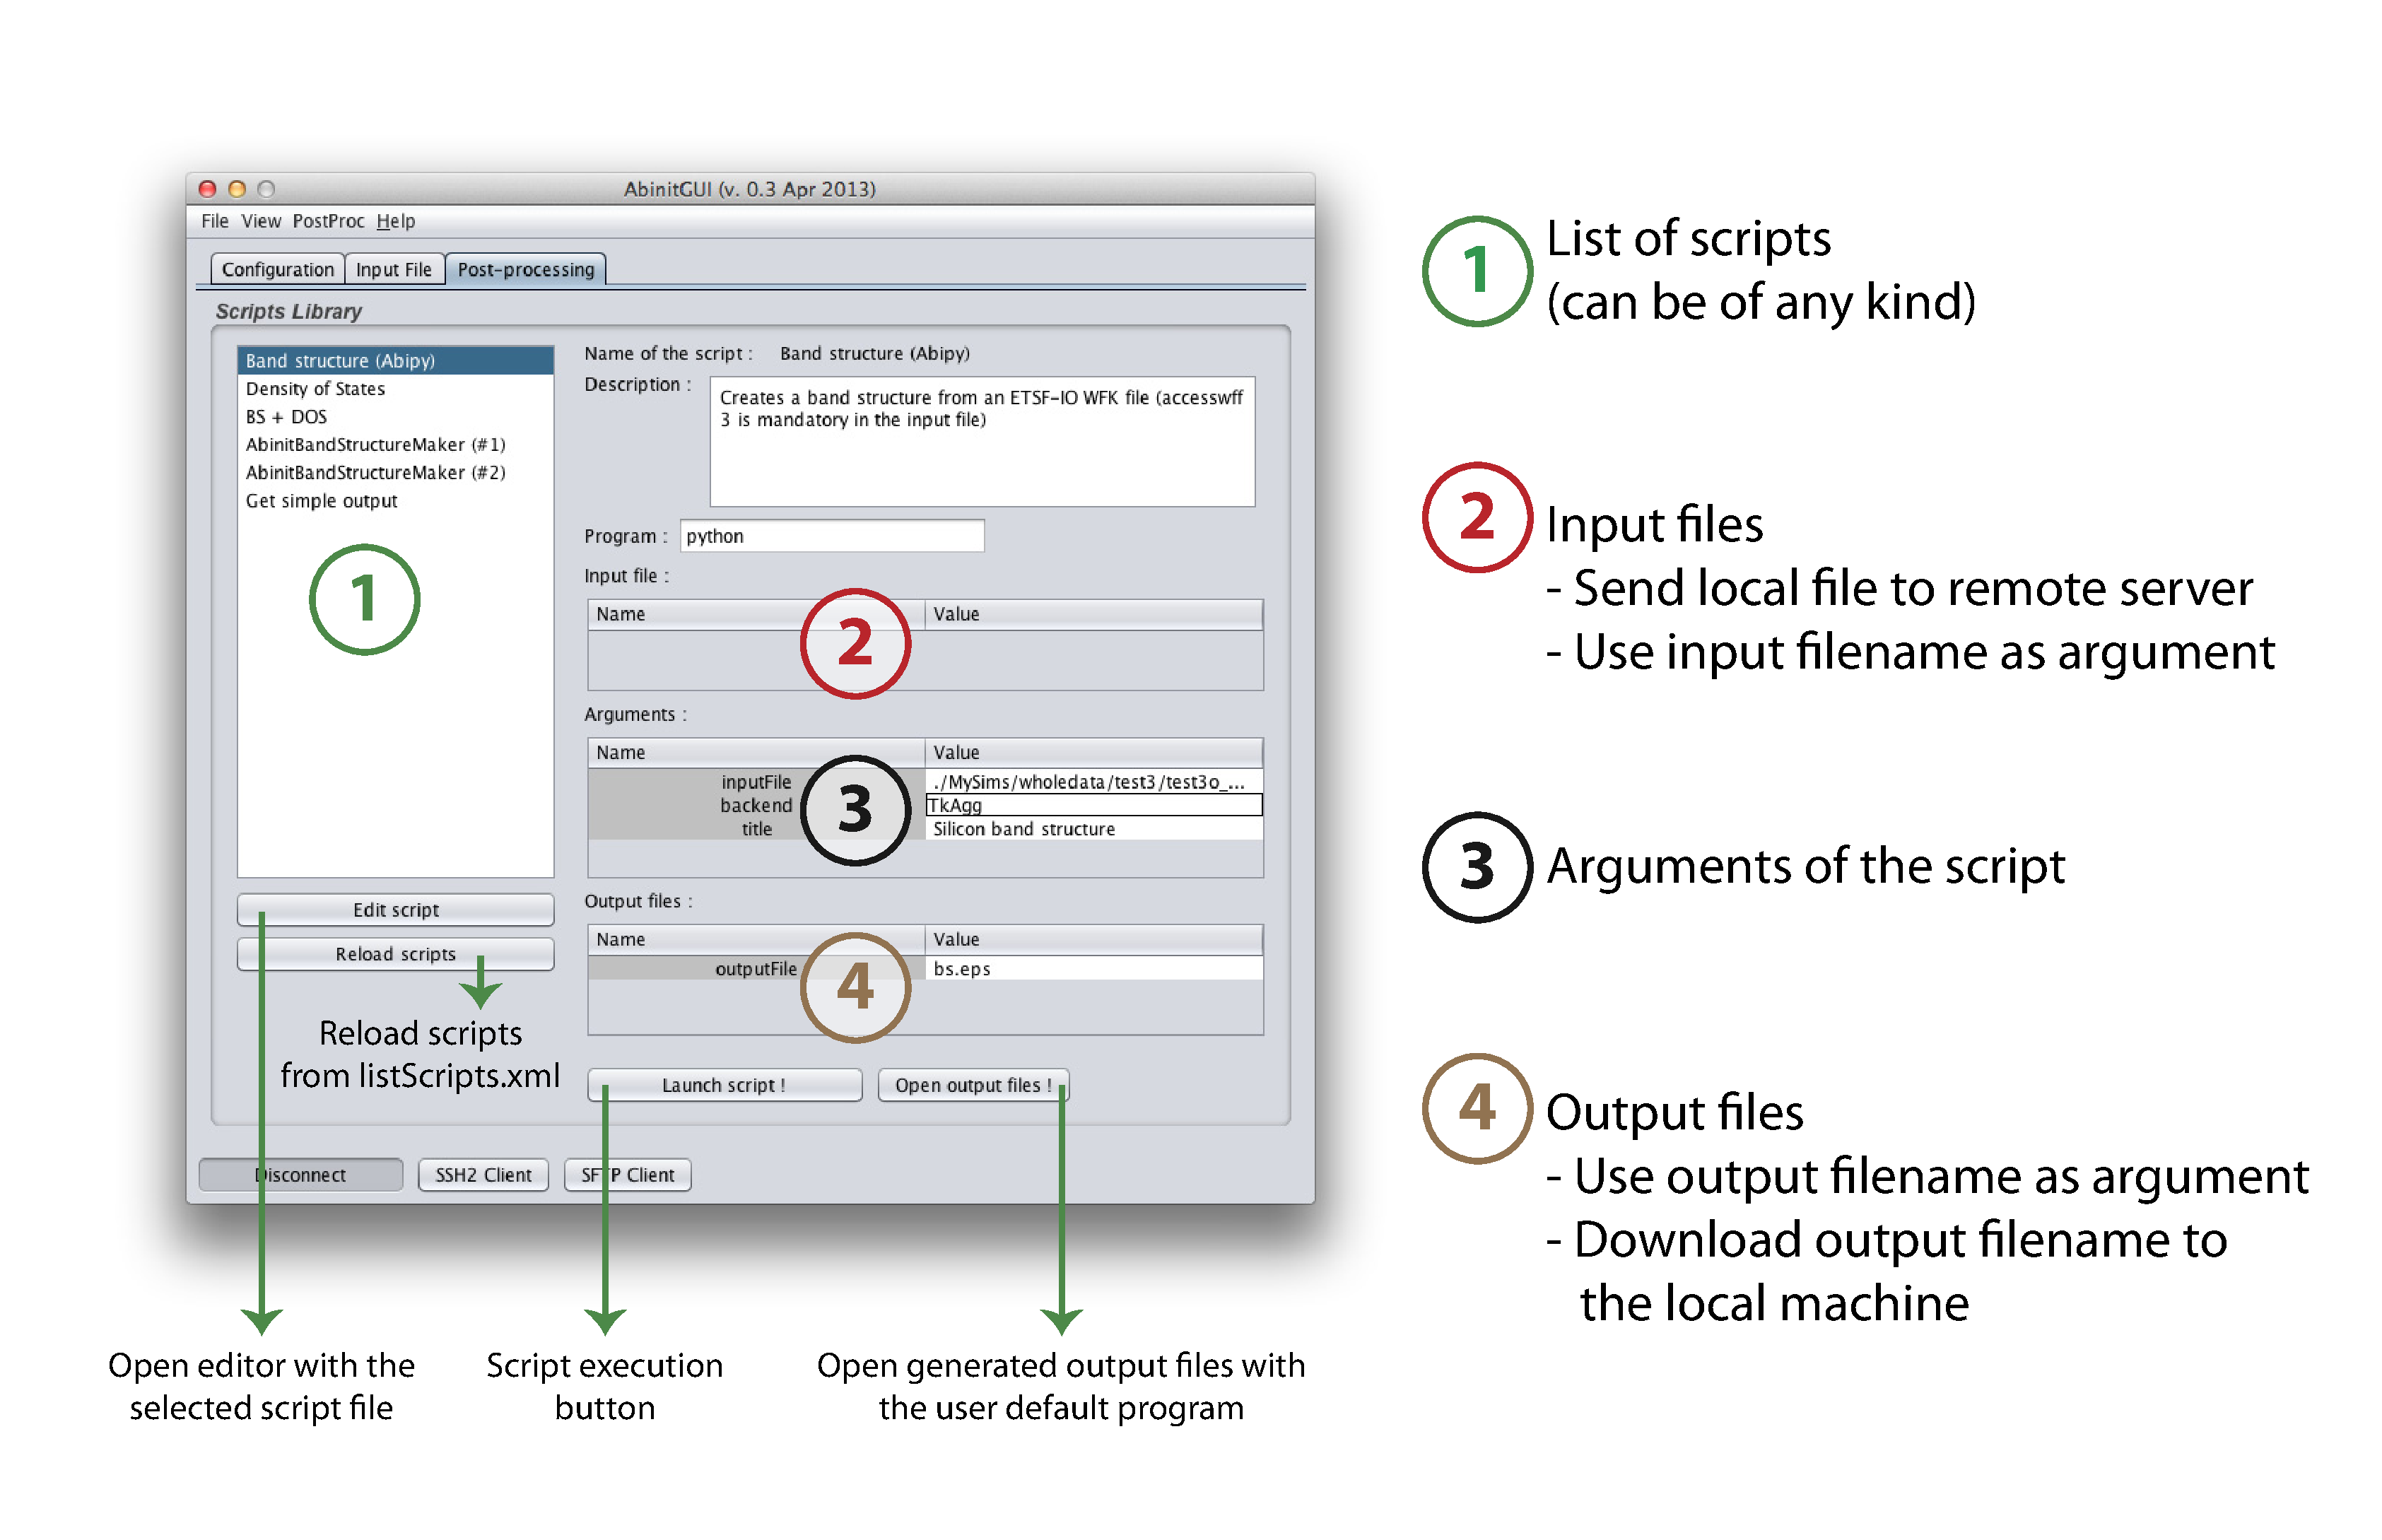
\includegraphics[height=8.25cm]{f7a}\\}
\only<2>{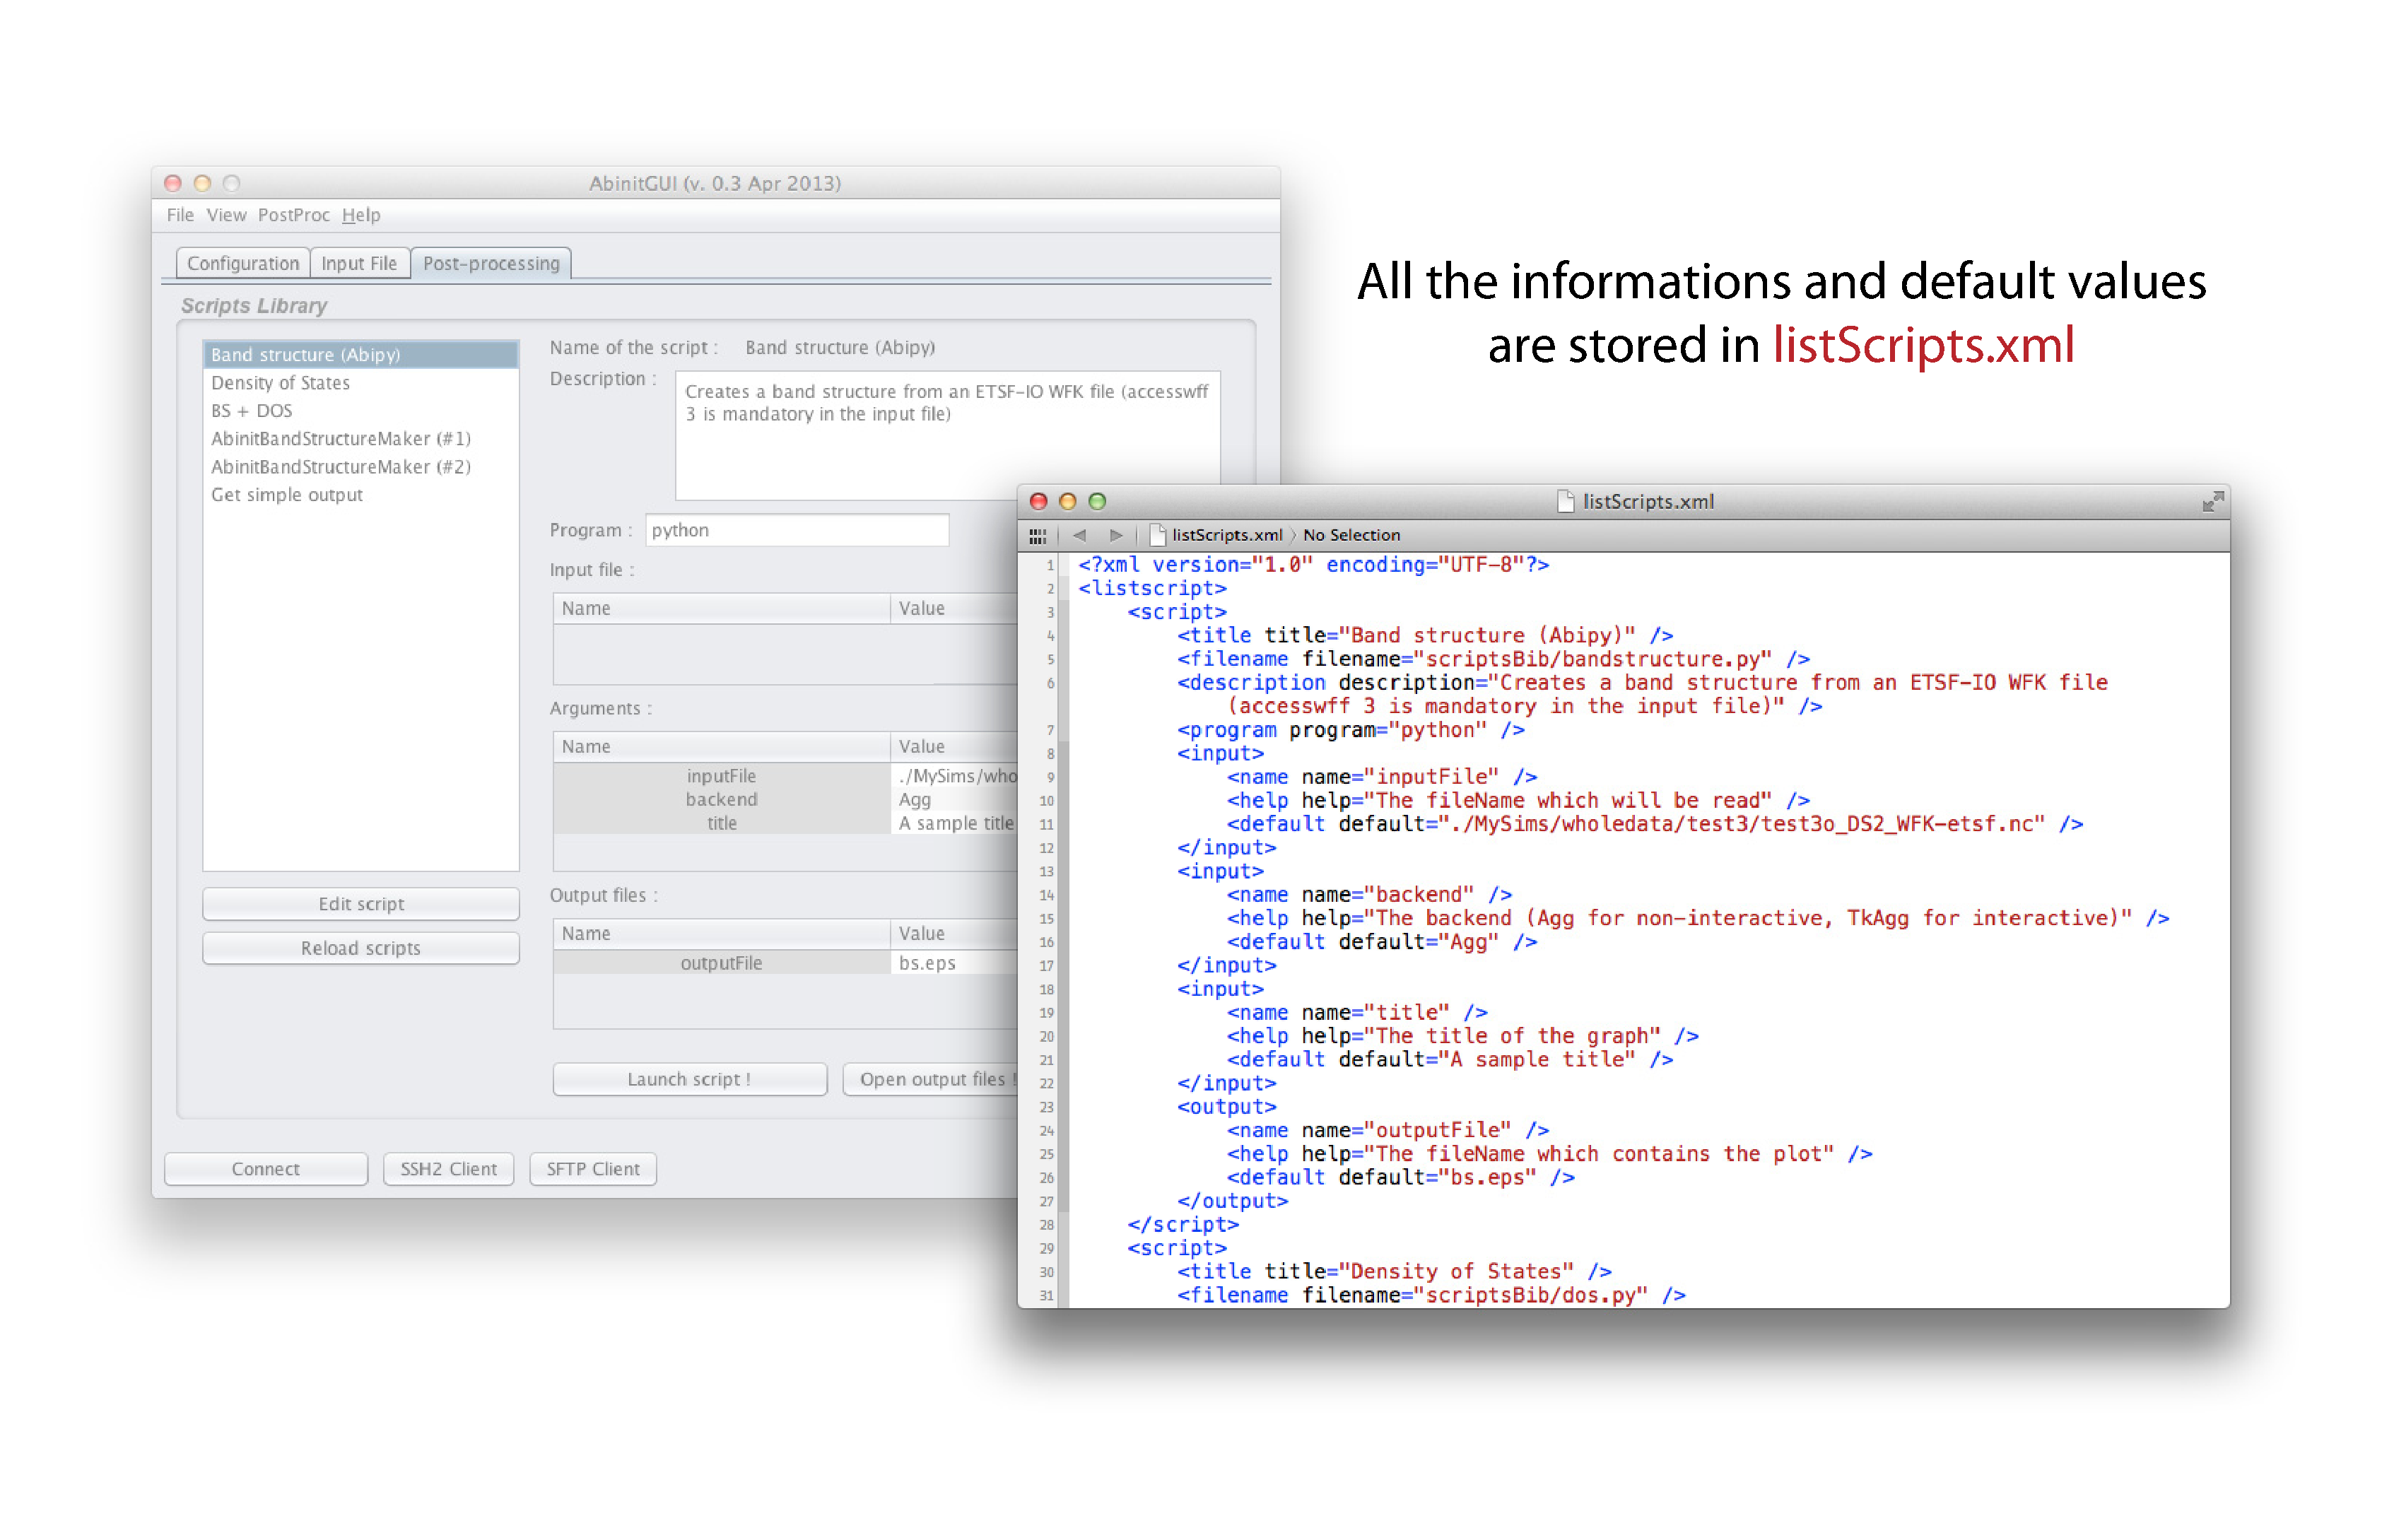
\includegraphics[height=8.25cm]{f7b}\\}
\only<3>{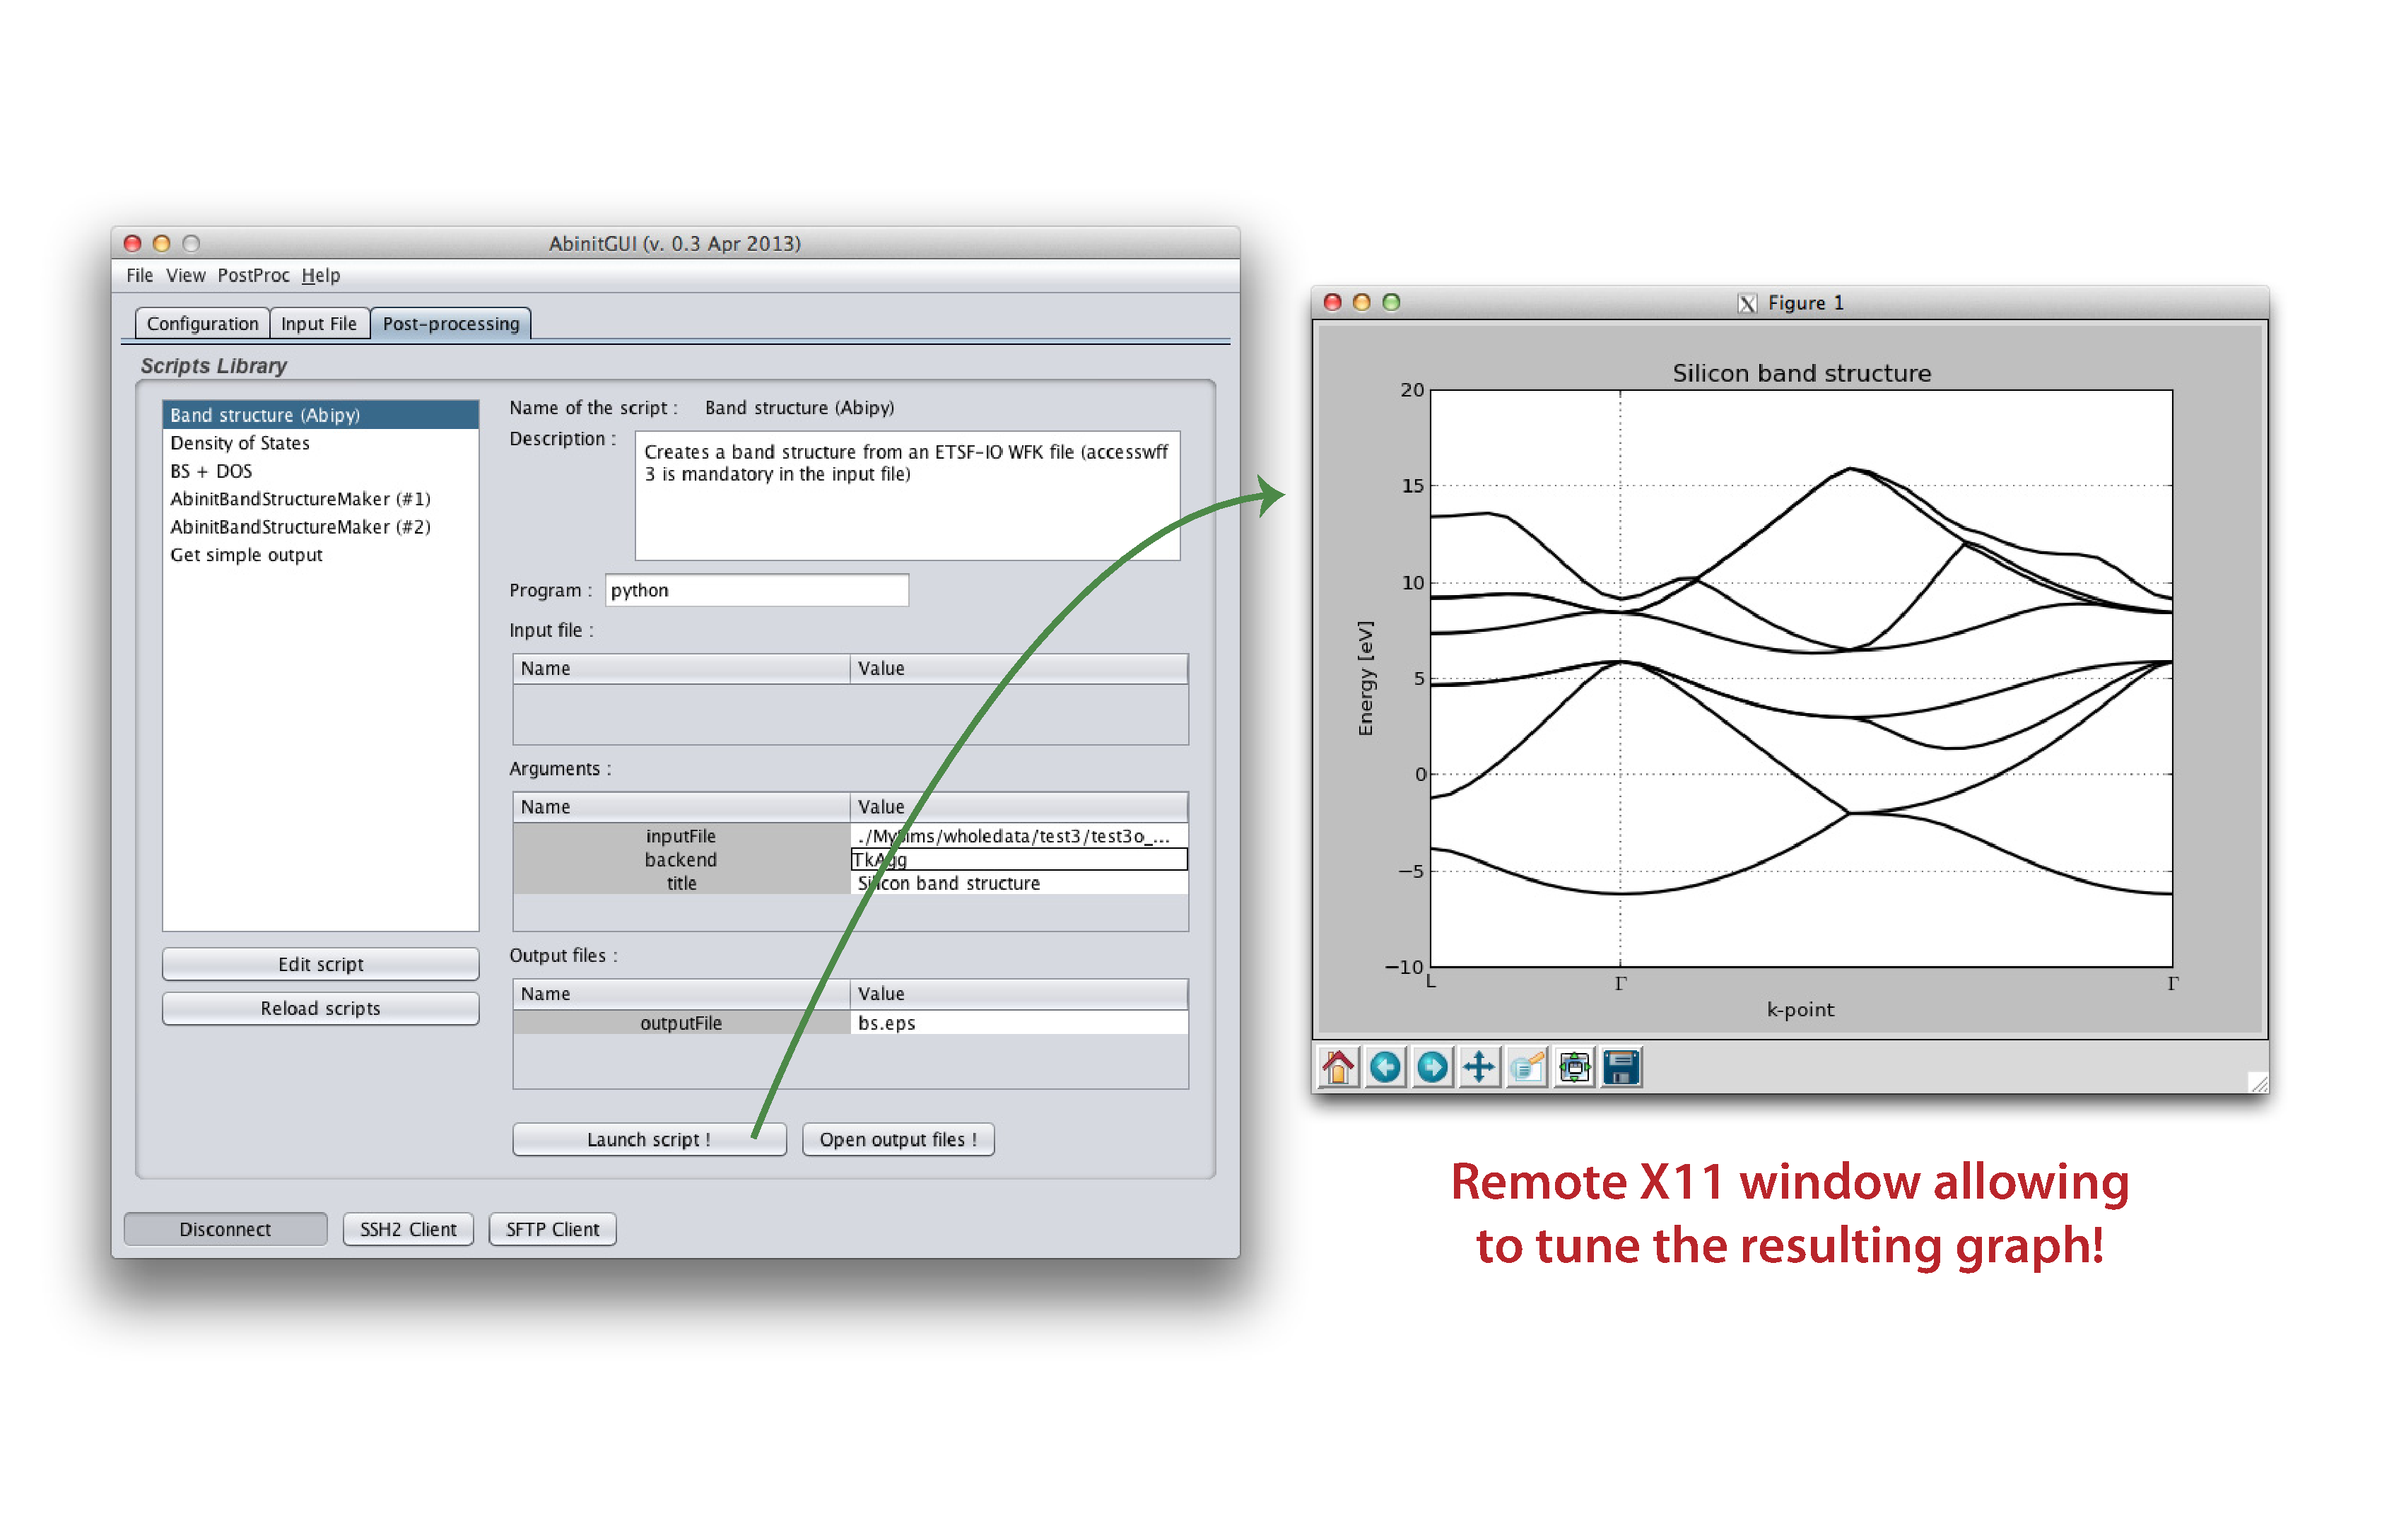
\includegraphics[height=8.25cm]{f7a_bis}\\}
\only<4>{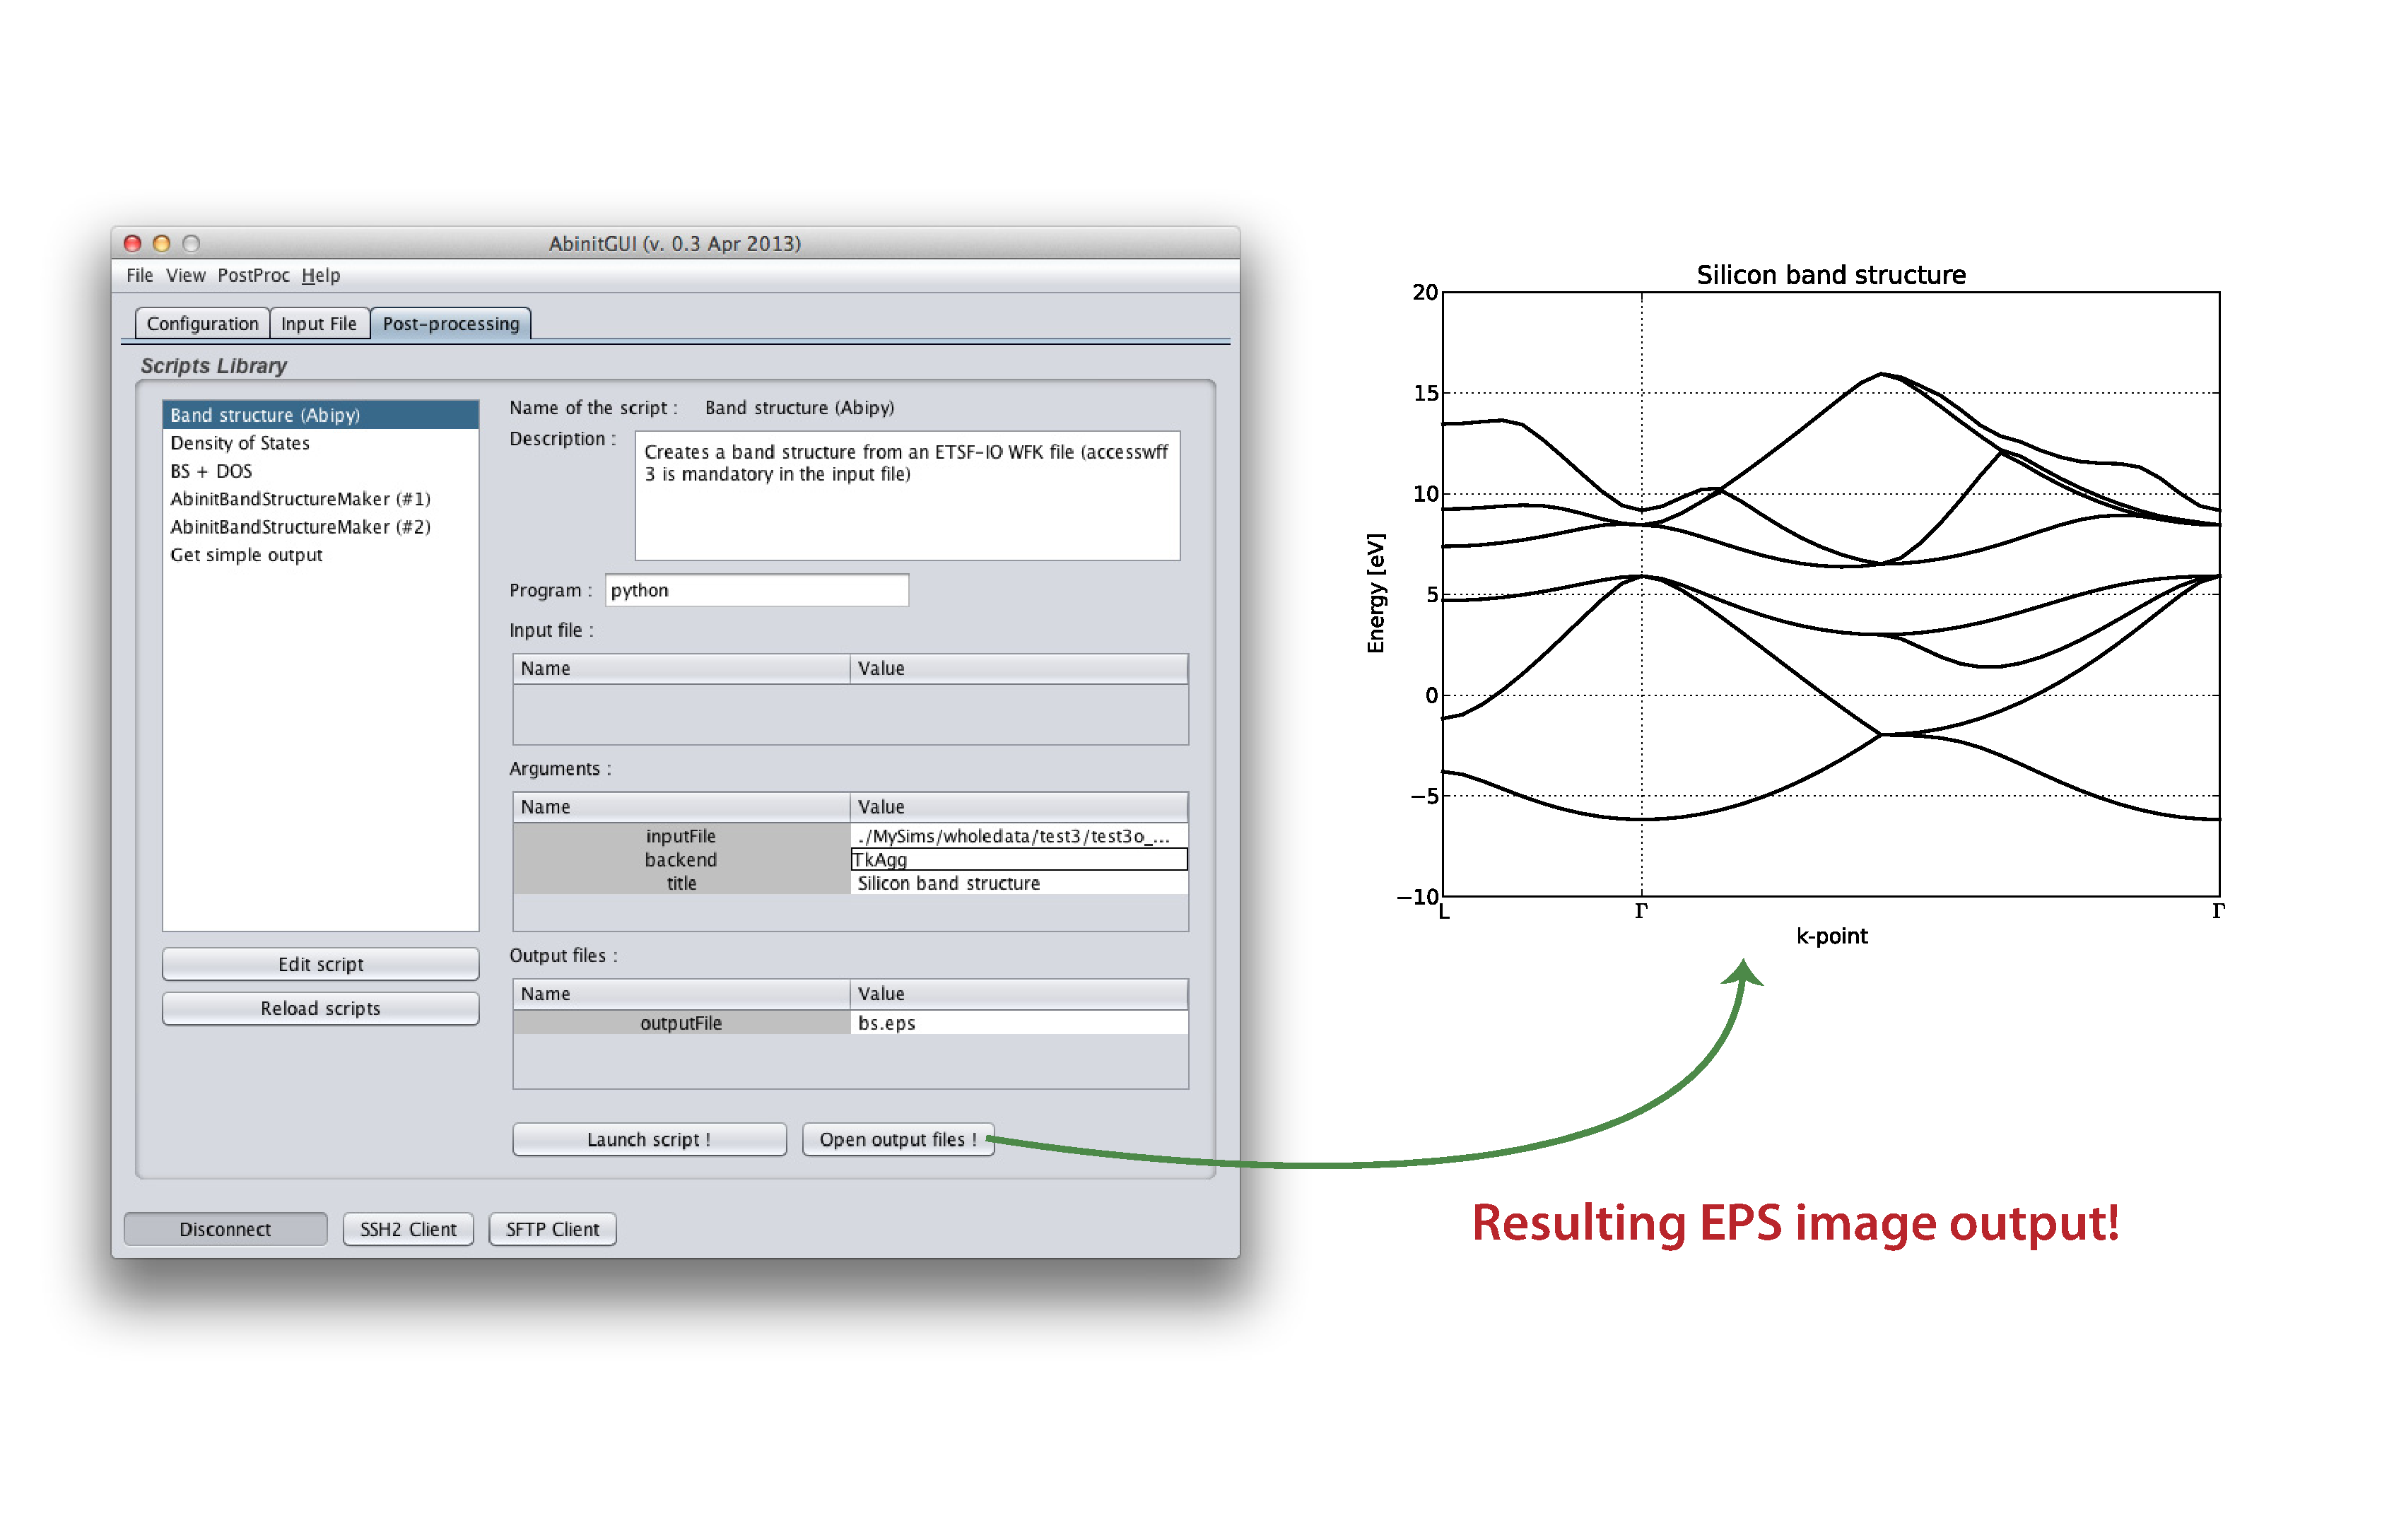
\includegraphics[height=8.25cm]{f7a_bis2}\\}
\end{frame}

%%% ----------- F8
%\begin{frame}
% \frametitle{Post-processing (2)}
%\centering
%\only<1>{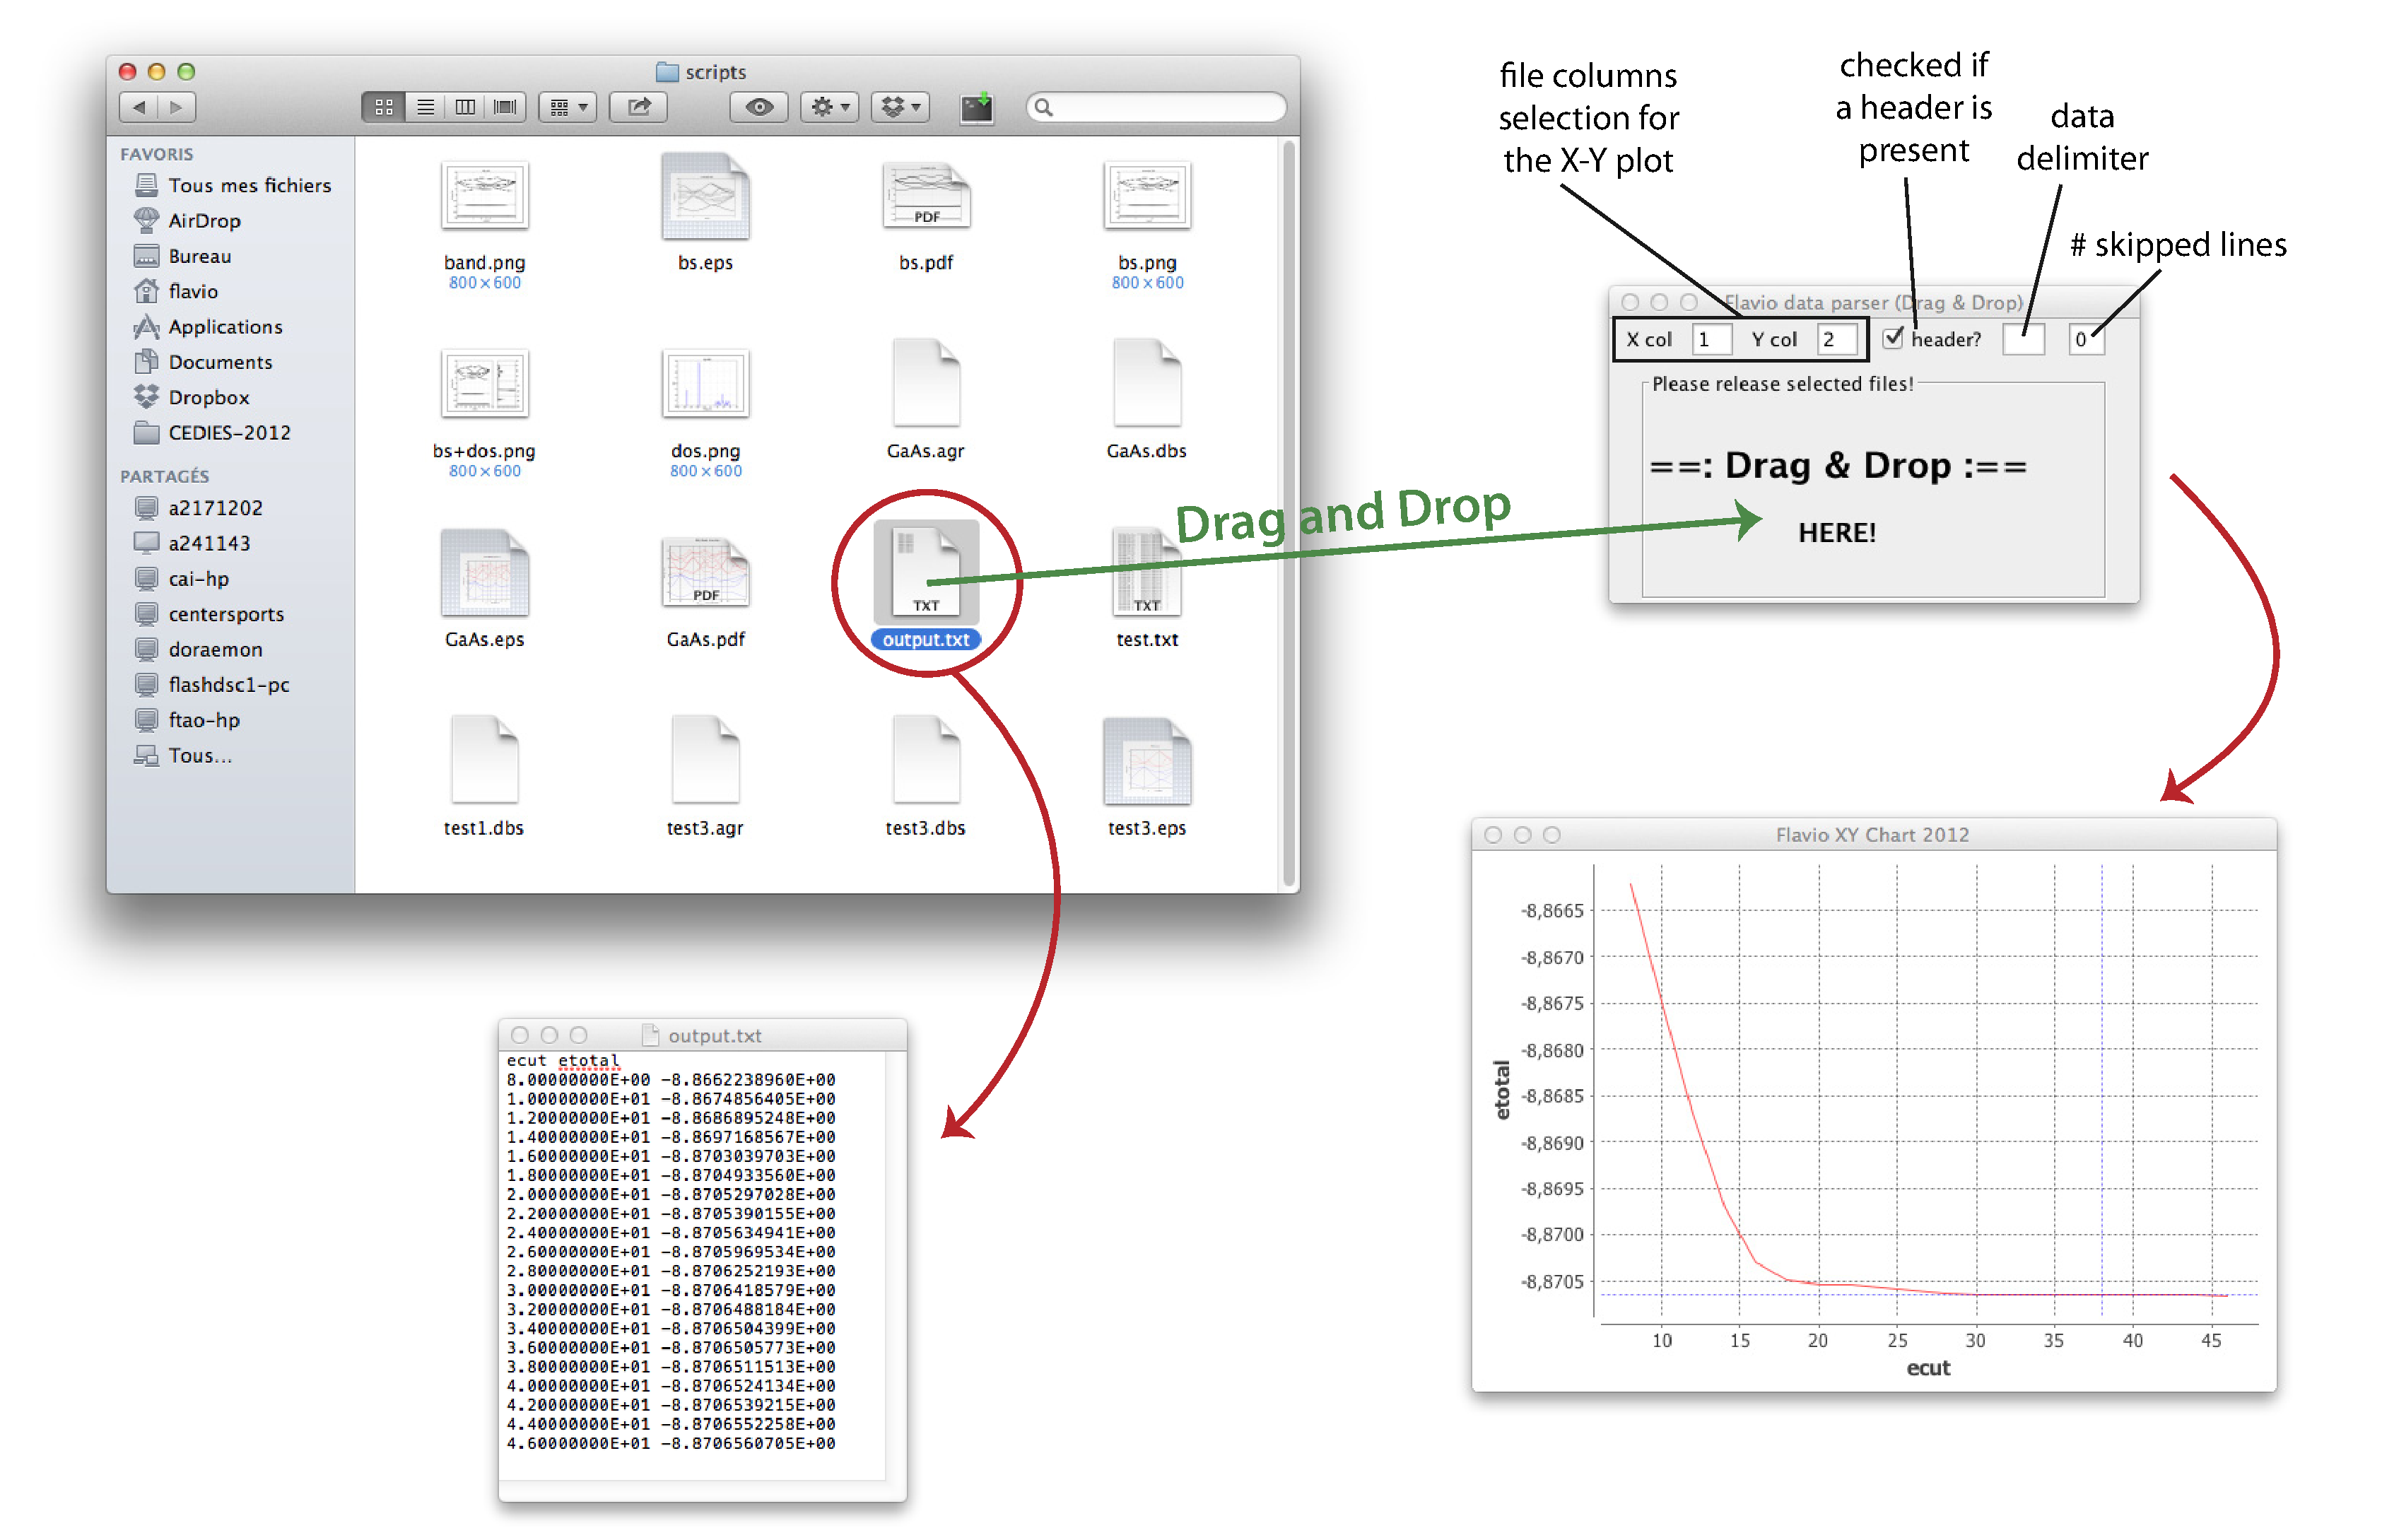
\includegraphics[height=8.25cm]{f8a}\\}
%\end{frame}

%%% ----------- F9
%\begin{frame}
% \frametitle{Post-processing (3)}
%\centering
%\only<1>{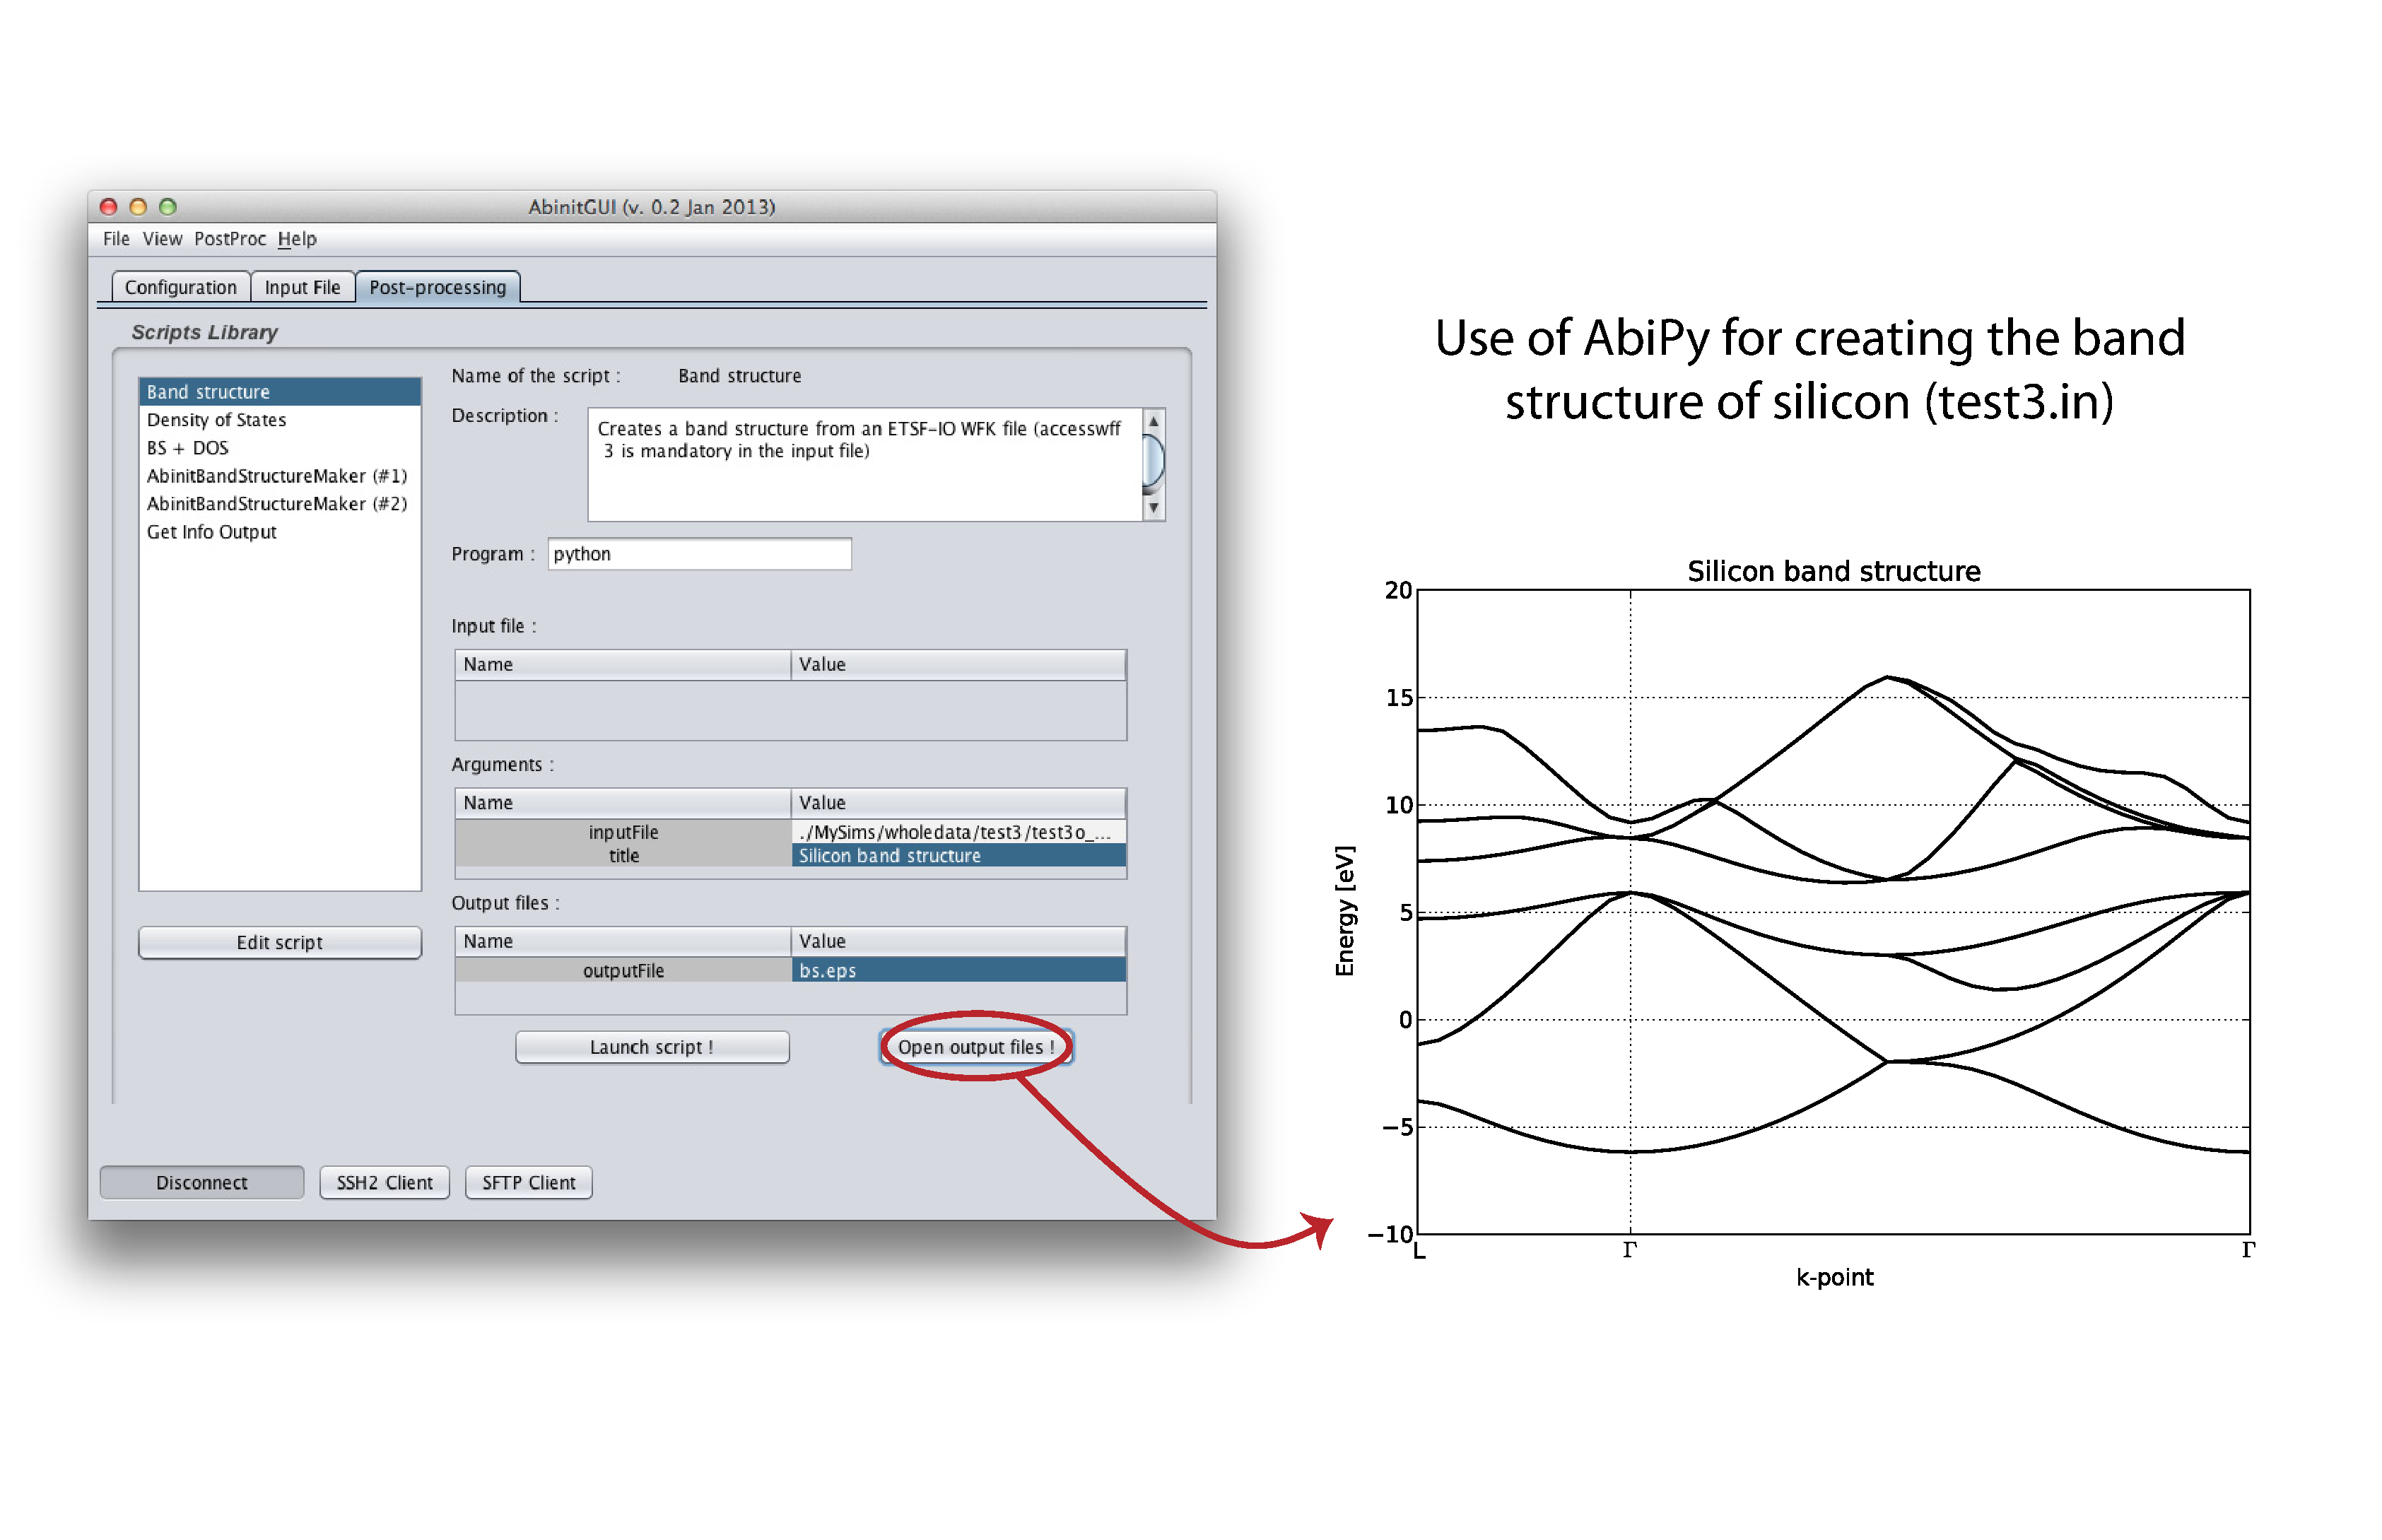
\includegraphics[height=8.25cm]{f9}\\}
%\end{frame}

%%% ------------ Supp
%\begin{frame}
% \frametitle{Gateway \& SGE configuration}
% \centering
% \only<1>{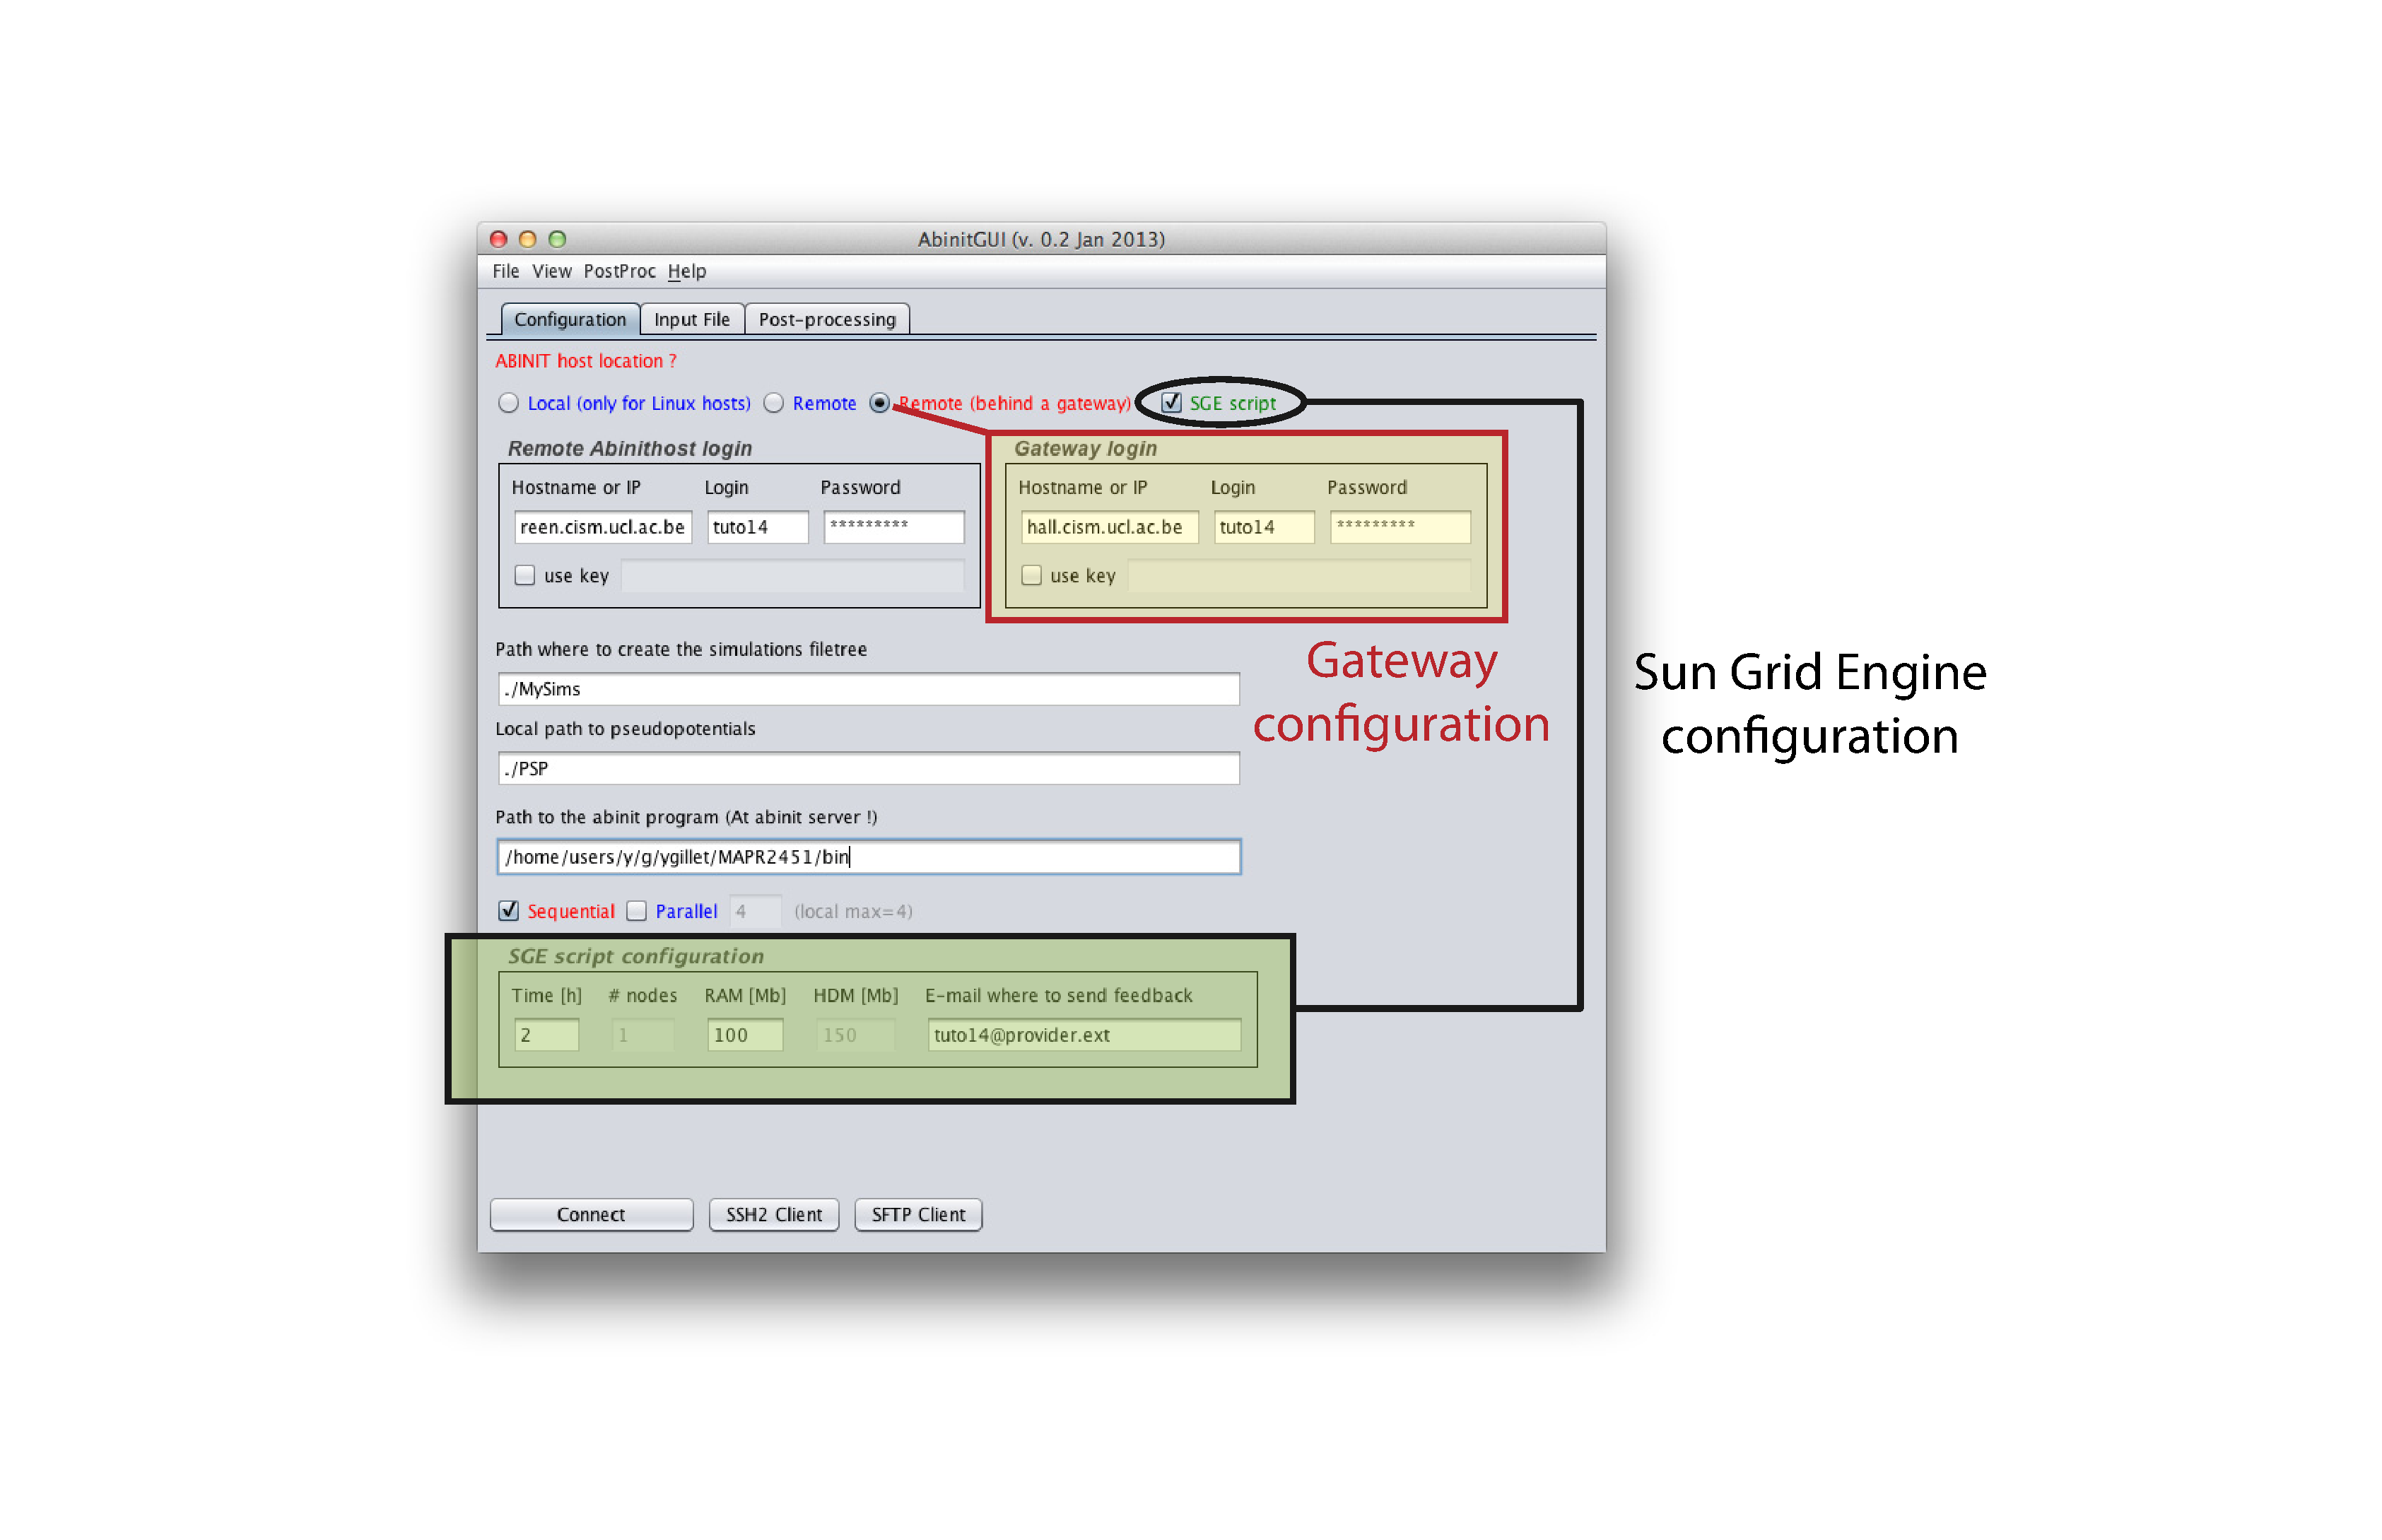
\includegraphics[height=8.25cm]{f10}\\}
%\end{frame}


%\setbeamertemplate{footline}{}
%
%%% ----------- I1
%\begin{frame}
%\end{frame}
% 
% \addtocounter{framenumber}{-1}
%\setbeamertemplate{footline}{%
%\leavevmode\hbox{%
% 
% \begin{beamercolorbox}[wd=.32\paperwidth,ht=2.5ex,dp=1.125ex,leftskip=.0cm plus1fill,rightskip=.0cm]{author in head/foot}%
%\centering
%%\usebeamerfont{author in head/foot}{{\insertshortauthor} (UCL)}
%\usebeamerfont{author in head/foot}{F. Abreu Araujo, Y. Gillet}
%\end{beamercolorbox}%
%
%\begin{beamercolorbox}[wd=.32\paperwidth,ht=2.5ex,dp=1.125ex,leftskip=.0cm,rightskip=.0cm plus1fil]{title in head/foot}%
%\centering
%\usebeamerfont{title in head/foot}\centering AbinitGUI%
%\end{beamercolorbox}%
%
%\begin{beamercolorbox}[wd=.32\paperwidth,ht=2.5ex,dp=1.125ex,leftskip=.0cm,rightskip=.0cm plus1fil]{author in head/foot}%
%\centering
%\usebeamerfont{author in head/foot}\centering Dinard, April 17, 2013%\today
%\end{beamercolorbox}%
%
%\begin{beamercolorbox}[wd=.04\paperwidth,ht=2.5ex,dp=1.125ex,leftskip=.0cm,rightskip=.0cm plus1fil]{title in head/foot}%
%\centering
%\usebeamerfont{author in head/foot}\insertframenumber
%\end{beamercolorbox}}%
%\vskip0pt%
%}


%% ----------- Summary
\begin{frame}
 \frametitle{Conclusion}
 \centering
 \only<1>{
\includegraphics[height=8.25cm]{f11}\\}
\end{frame}

\begin{frame}
 \frametitle{Perspectives}
 \centering
 \only<1>{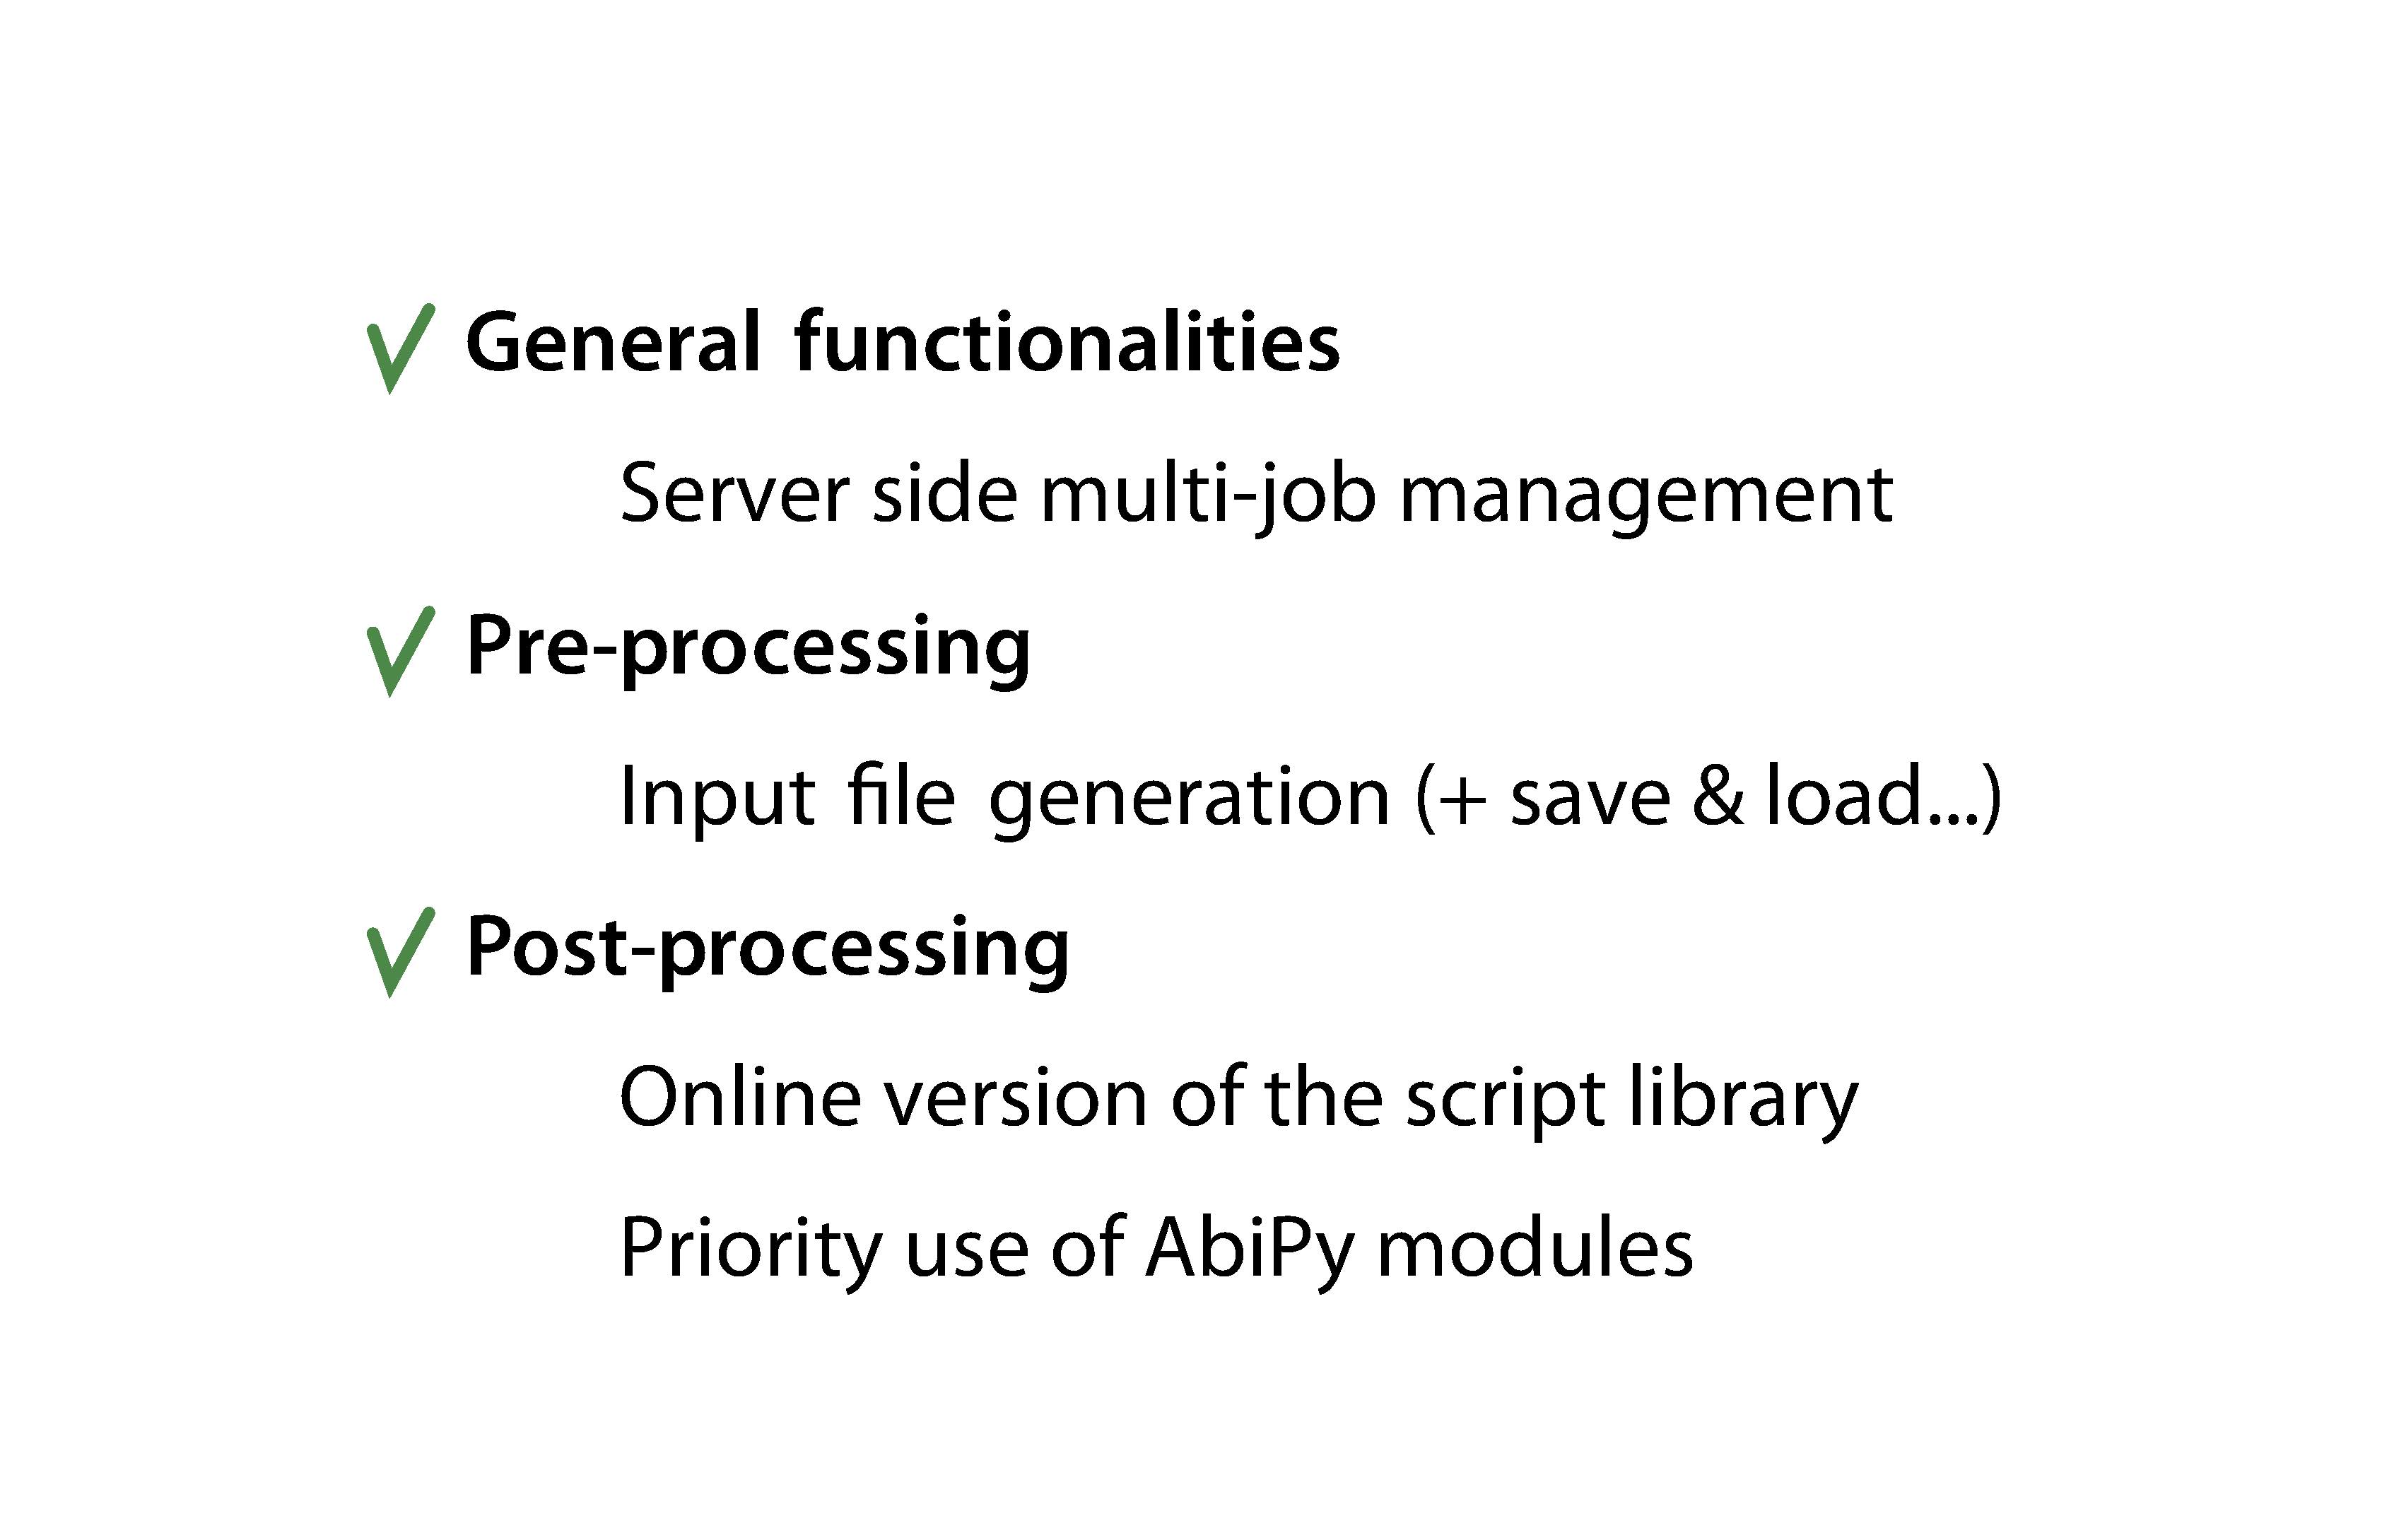
\includegraphics[height=8.25cm]{f12}\\}
\end{frame}

%\begin{frame}
% \frametitle{Many thanks to:}
% \centering
% \only<1>{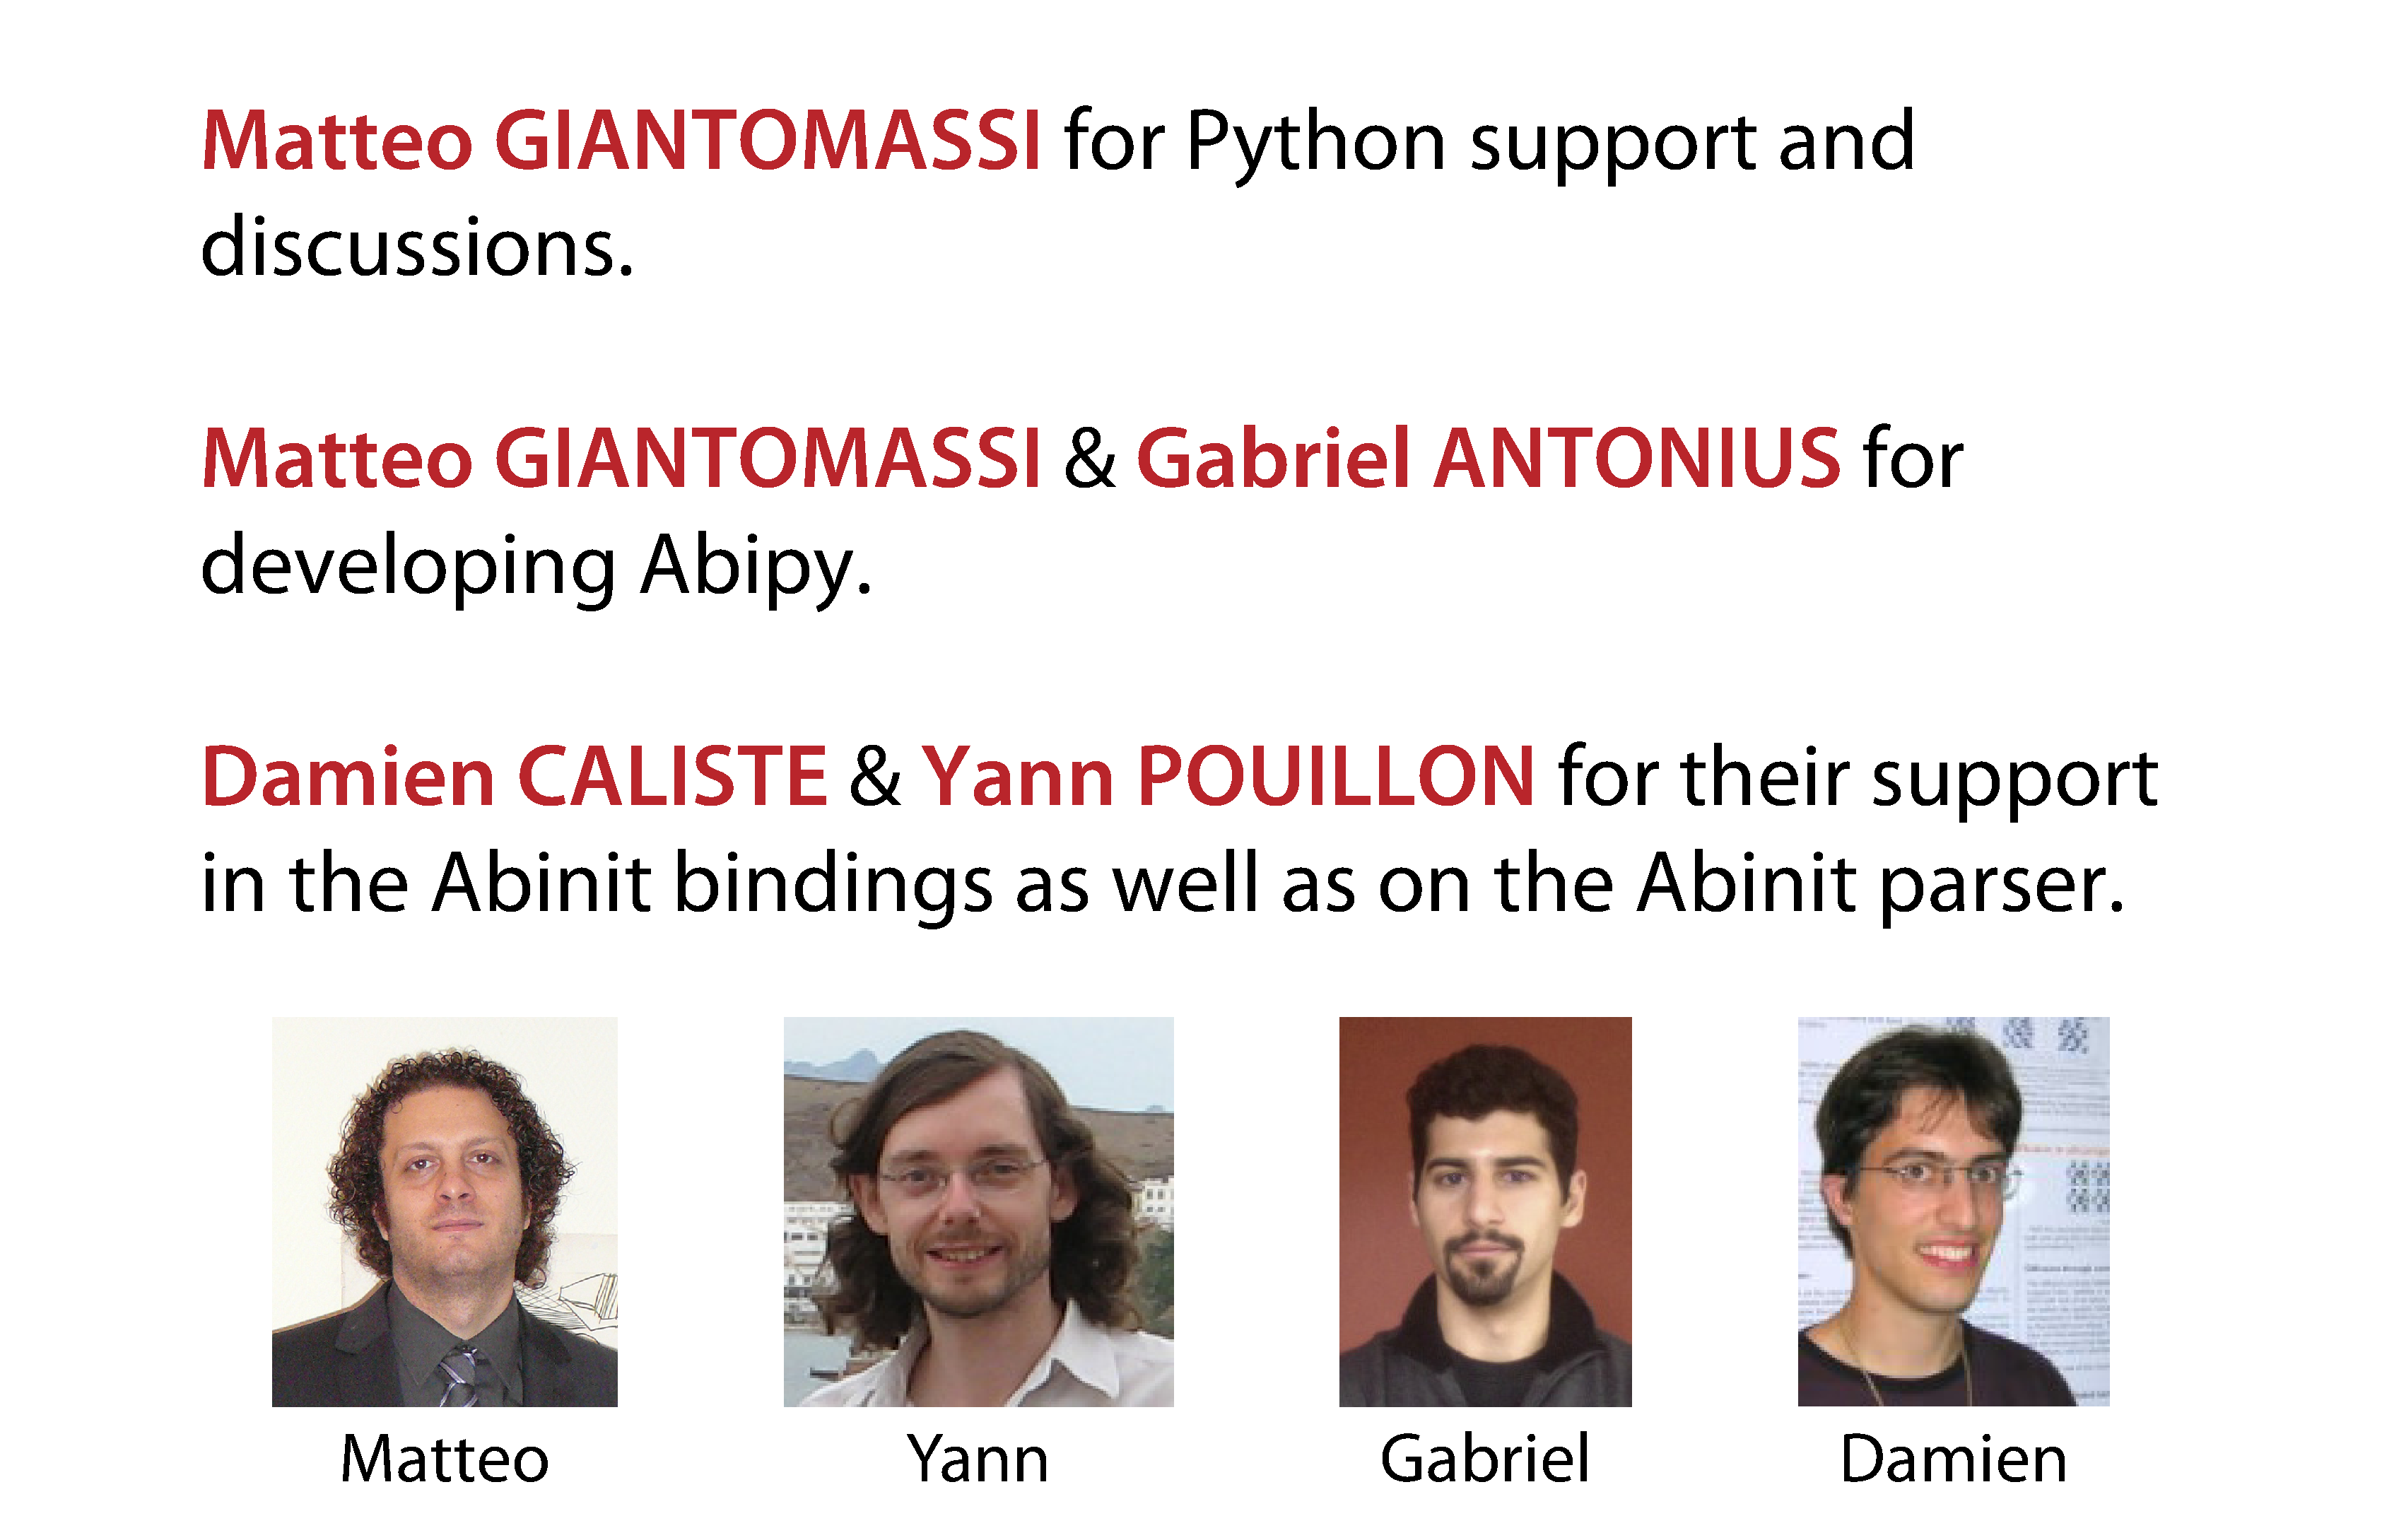
\includegraphics[height=8.25cm]{f13}\\}
%\end{frame}

\end{document}
